\documentclass[dissertation.tex]{subfiles} 
\begin{document}

\chapter{Data Analysis}
\label{chap:Data Analysis}

The signature of GGM SUSY particle production in this search is an excess of two-photon events with high \MET.  \MET is reconstructed using the particle flow algorithm as described in Sec.~\ref{sec:MET}.  Candidate two-photon events, as well as control events, are selected according to the offline object criteria presented in Secs.~\ref{sec:Photons} ,~\ref{sec:Electrons}, and~\ref{sec:Jets}; the event quality criteria in Sec.~\ref{sec:Event Quality}; and the trigger requirements in Sec.~\ref{sec:HLT}.  These are summarized in Table~\ref{tab:selection_summary}.

\begin{table}[hcbp]
\caption{Selection criteria for $\gamma\gamma$, $e\gamma$, $ee$, and $\mathit{ff}$ events.}
\centering
\begin{tabular}{|c|c|c|c|c|}
\hline
\multirow{2}{*}{Variable} & \multicolumn{4}{c|}{Cut} \\
\cline{2-5}
& $\gamma\gamma$ & $e\gamma$ & $ee$ & $\mathit{ff}$ \\
\hline
\hline
HLT match & IsoVL & IsoVL & IsoVL & IsoVL $||$ R9Id \\
\hline
$E_{T}$ & \begin{tabular}[c]{@{}c@{}}$> 40$/\\$> 25$ GeV\end{tabular} & \begin{tabular}[c]{@{}c@{}}$> 40$/\\$> 25$ GeV\end{tabular} & \begin{tabular}[c]{@{}c@{}}$> 40$/\\$> 25$ GeV\end{tabular} & \begin{tabular}[c]{@{}c@{}}$> 40$/\\$> 25$ GeV\end{tabular} \\
\hline
SC $|\eta|$ & $< 1.4442$ & $<1.4442$ & $< 1.4442$ & $<1.4442$ \\
\hline
$H/E$ & $<0.05$ & $<0.05$ & $<0.05$ & $<0.05$ \\
\hline
$R9$ & $< 1$ & $< 1$ & $< 1$ & $< 1$ \\
\hline
Pixel seed & No/No & Yes/No & Yes/Yes & No/No \\
\hline
$I_{\mathrm{comb}}$, $\sigma_{i\eta i\eta}$ & \begin{tabular}[c]{@{}c@{}}$< 6$ GeV \&\&\\$< 0.011$\end{tabular} & \begin{tabular}[c]{@{}c@{}}$< 6$ GeV \&\&\\$< 0.011$\end{tabular} & \begin{tabular}[c]{@{}c@{}}$< 6$ GeV \&\&\\$< 0.011$\end{tabular} & \begin{tabular}[c]{@{}c@{}}$< 20$ GeV \&\&\\($\geq 6$ GeV $||$\\$\geq 0.011$)\end{tabular} \\
\hline
JSON & Yes & Yes & Yes & Yes \\
\hline
No. good PVs & $\geq 1$ & $\geq 1$ & $\geq 1$ & $\geq 1$ \\
\hline
$\Delta R_{\mathrm{EM}}$ & $> 0.6$ & $> 0.6$ & $> 0.6$ & $> 0.6$ \\
\hline
$\Delta\phi_{\mathrm{EM}}$ & $\geq 0.05$ & $\geq 0.05$ & $\geq 0.05$ & $\geq 0.05$ \\
\hline
\end{tabular}
\label{tab:selection_summary}
\end{table}

This search utilizes 4.7 $\mbox{fb}^{-1}$ of CMS data collected during the period April-December 2011, corresponding to the following datasets \cite{DAS}:

\begin{itemize}
\item \verb+/Photon/Run2011A-05Jul2011ReReco-ECAL-v1/AOD+
\item \verb+/Photon/Run2011A-05Aug2011-v1/AOD+
\item \verb+/Photon/Run2011A-03Oct2011-v1/AOD+
\item \verb+/Photon/Run2011B-PromptReco-v1/AOD+
\end{itemize}

The search strategy is to model the backgrounds to the GGM SUSY signal using \MET shape templates derived from the control samples, and then to look for a high-\MET excess above the estimated background in the $\gamma\gamma$ sample.  There are two categories of backgrounds: QCD processes with no real \MET and electroweak processes with real \MET from neutrinos.  The relevant QCD background processes are multijet production with at least two jets faking photons, photon + jet production with at least one jet faking a photon, and diphoton production, and $Z$ production with a radiated photon where at least one of the $Z$ decay products (typically a jet) fakes a photon.  The relevant electroweak background processes, which are small compared to the QCD background, involve $W\rightarrow e\nu$ decay with a recoiling jet that fakes a photon or a real radiated photon (the $W$ may come from the decay of a top quark in $t\bar{t}$ events).  In both cases, the electron is misidentified as a photon due to a small inefficiency in reconstructing the electron pixel seed.  The main diagrams contributing to the QCD(electroweak) backgrounds are shown in Figure~\ref{fig:QCD_background_diagrams}(\ref{fig:EW_background_diagrams}).

\begin{figure}
	\centering
	\subfloat[Dijet production via $gg$ and $qg$ interactions.]{\label{fig:dijet}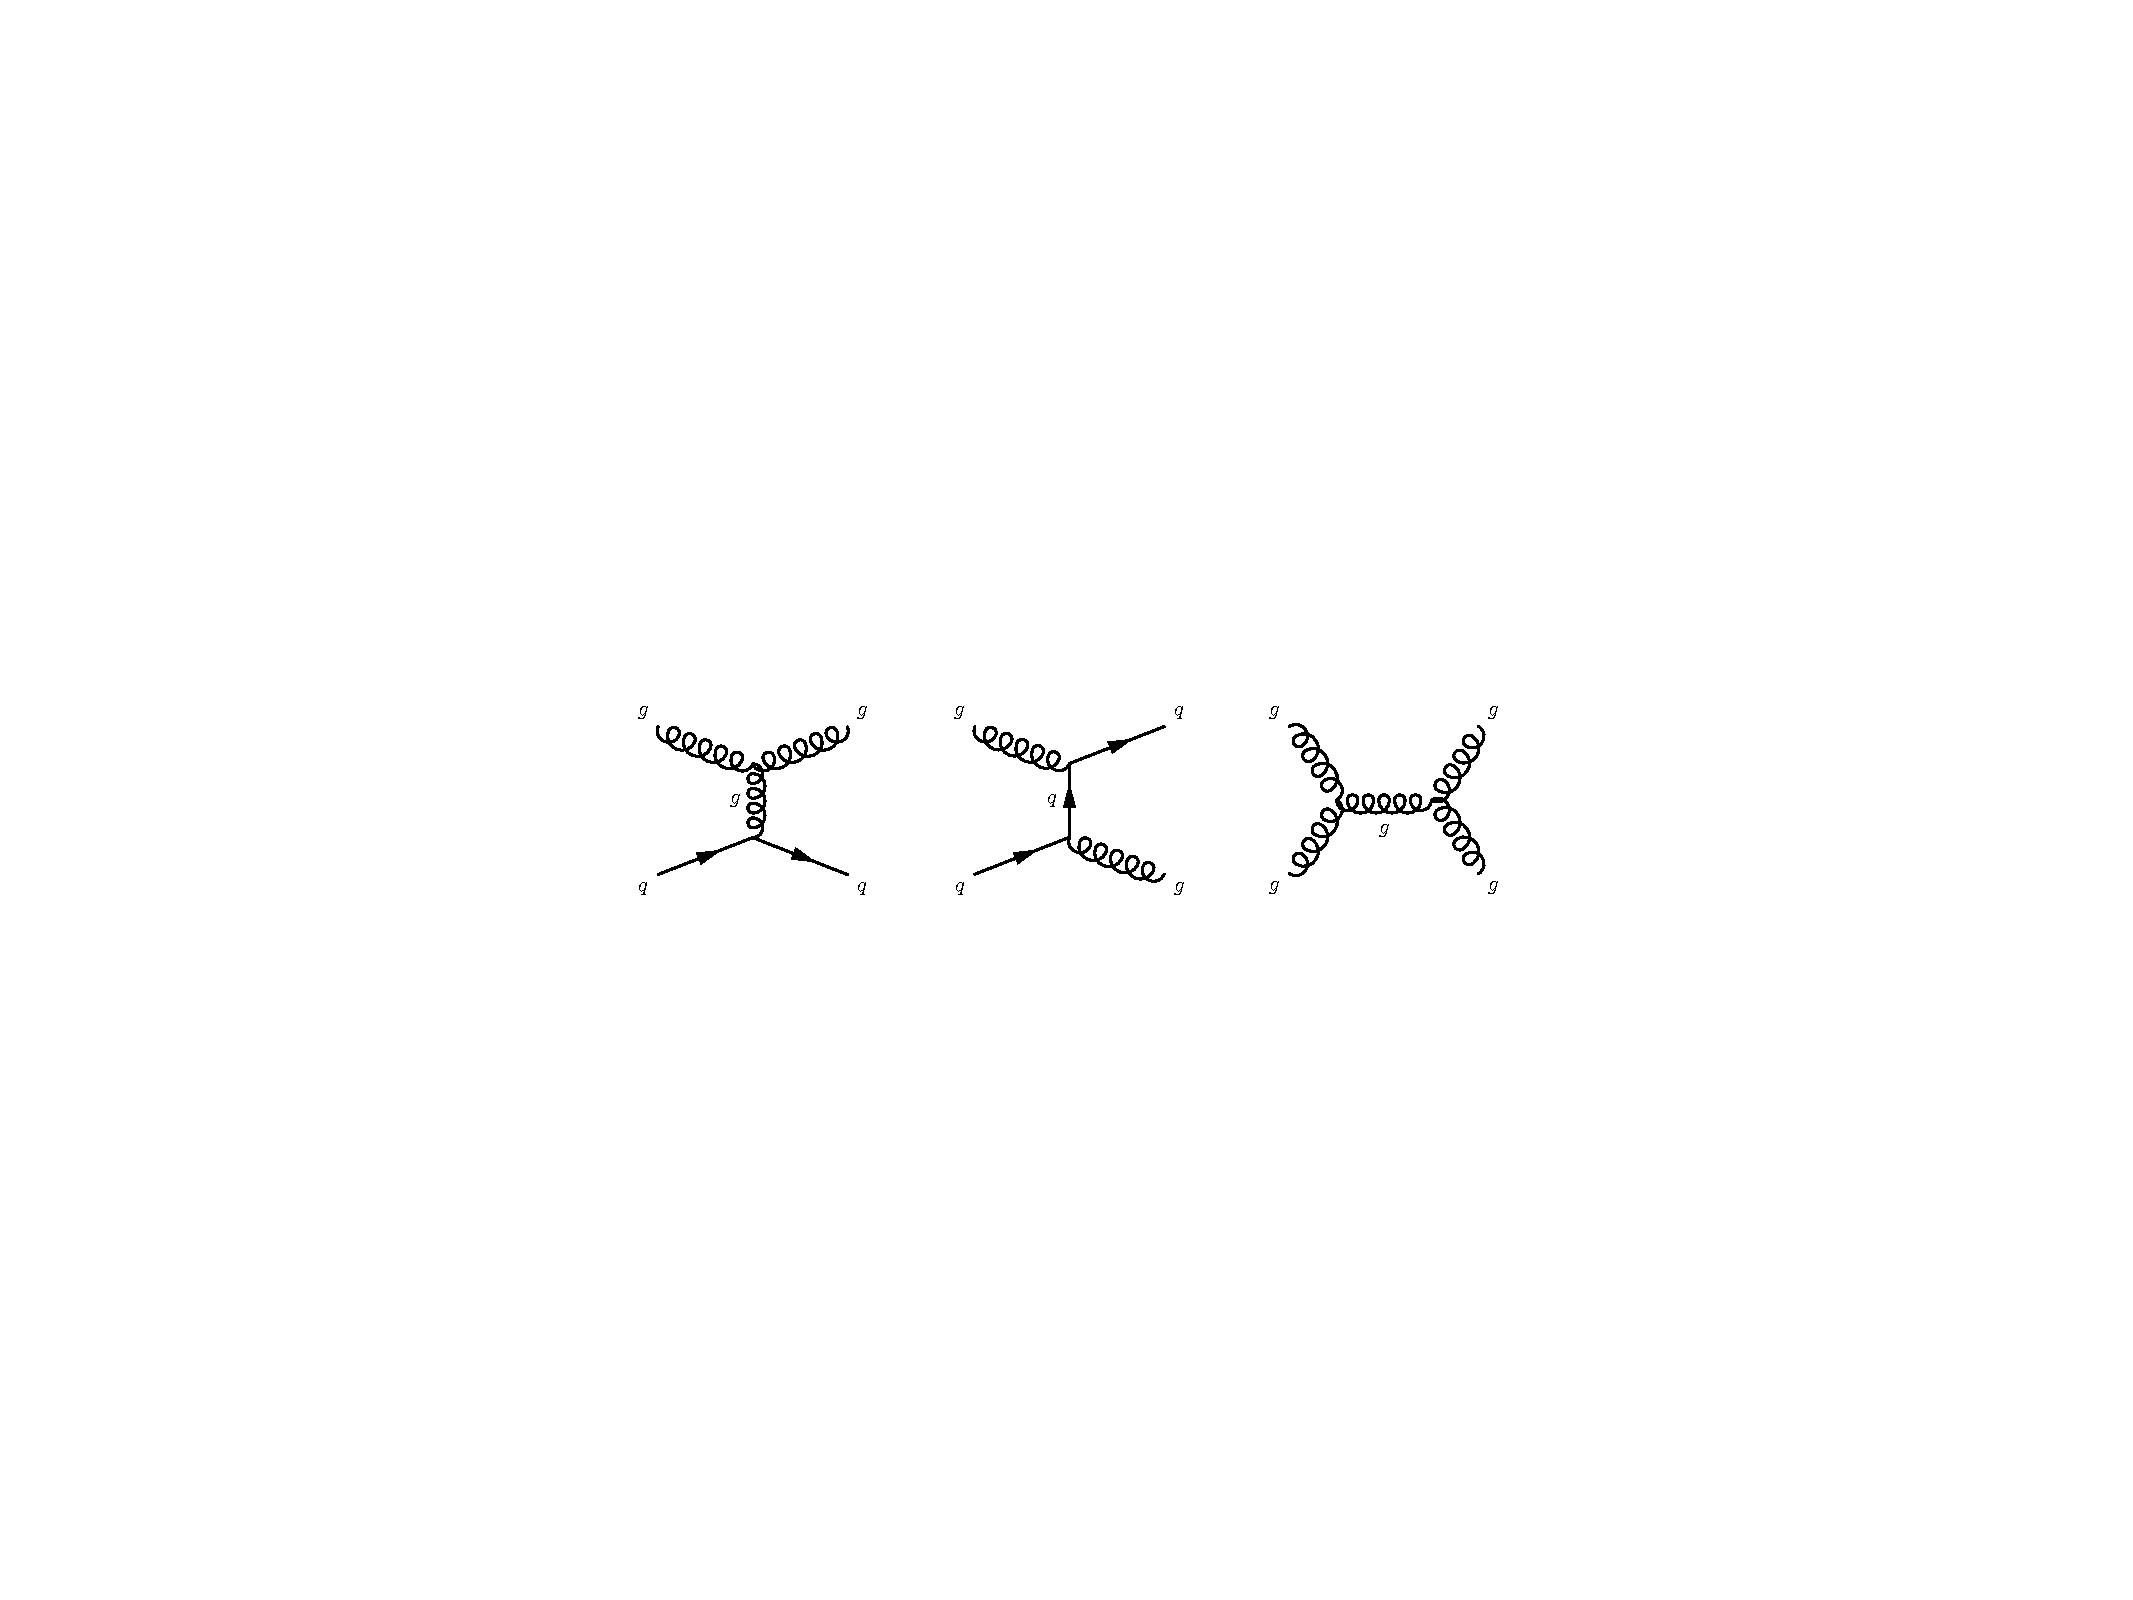
\includegraphics[scale=1.0]{dijet_cropped}}
	\\
	\subfloat[Photon + jet production via $qg$ interactions.]{\label{fig:qg_to_qa}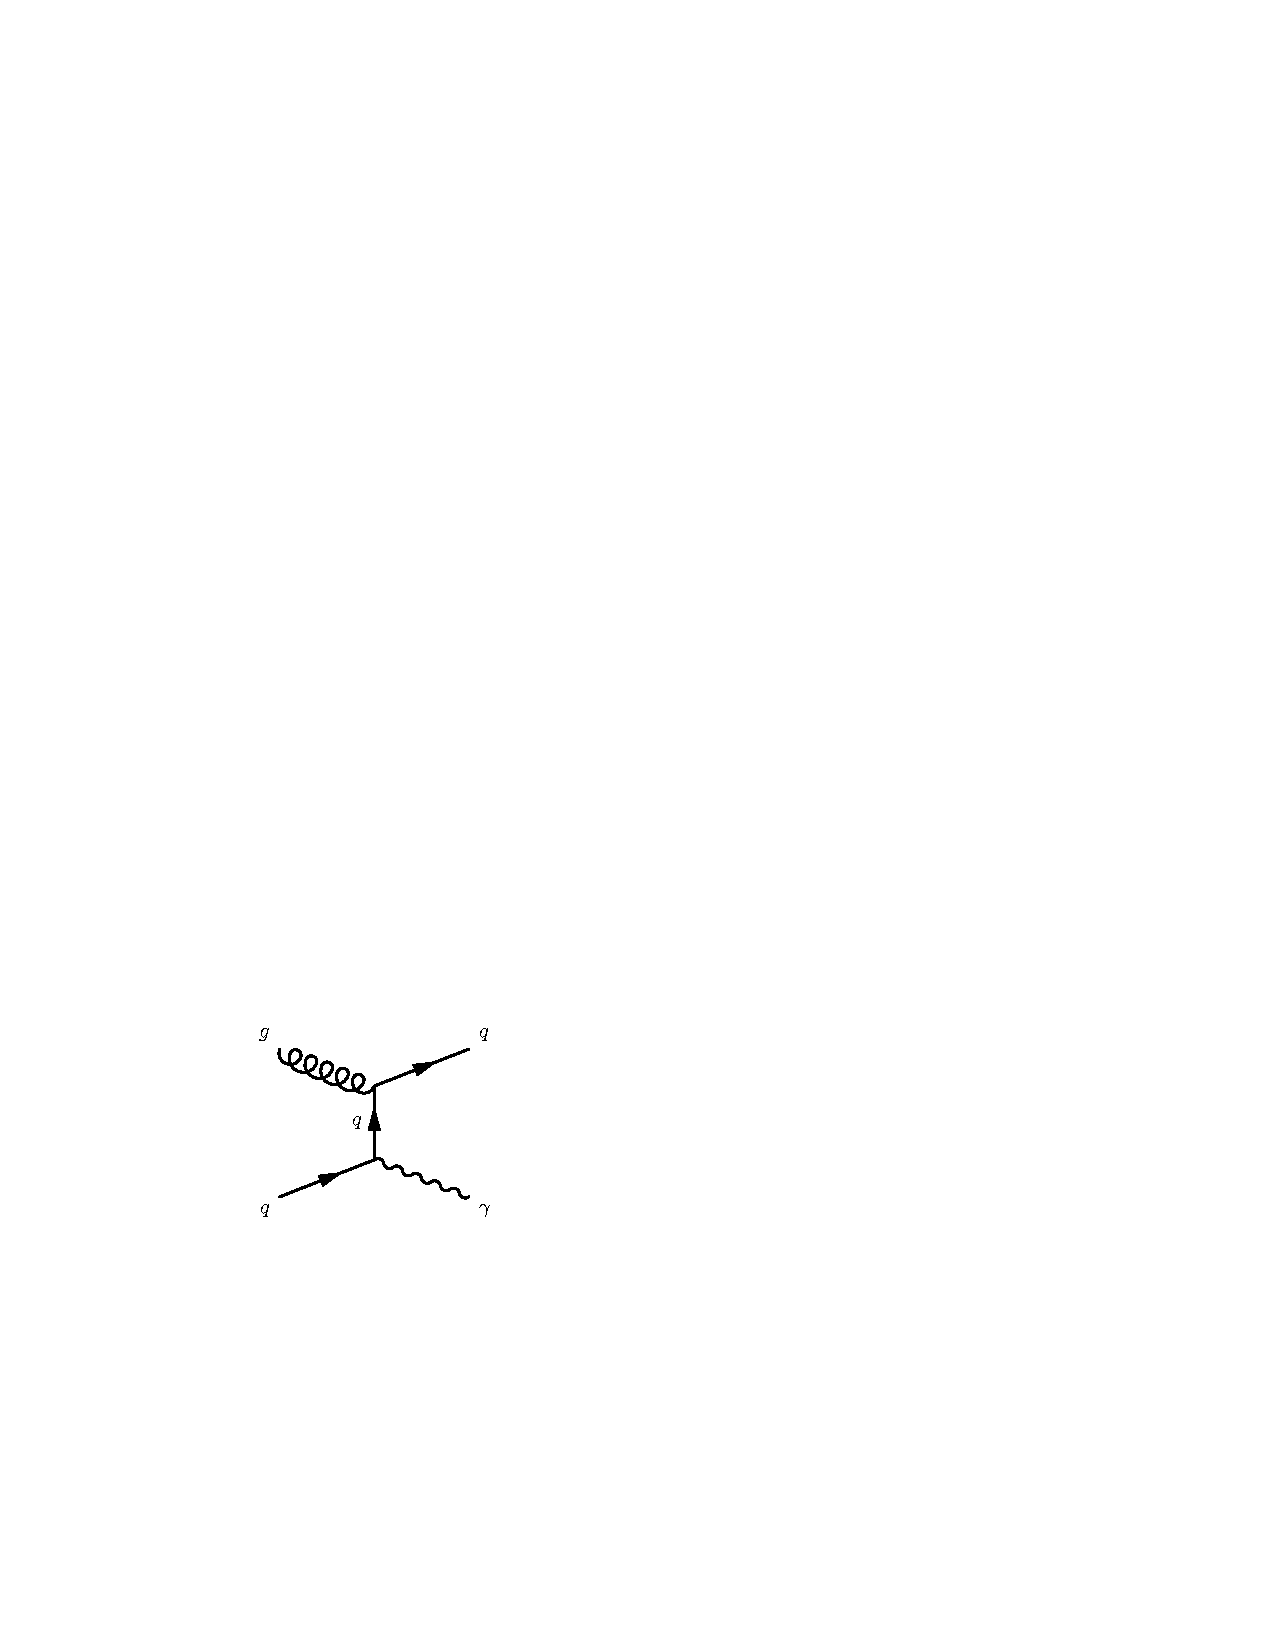
\includegraphics[scale=1.0]{qg_to_qa}}
	\hspace{1cm}
	\subfloat[Diphoton production via $q\bar{q}$ and $gg$ interactions.]{\label{fig:diphoton}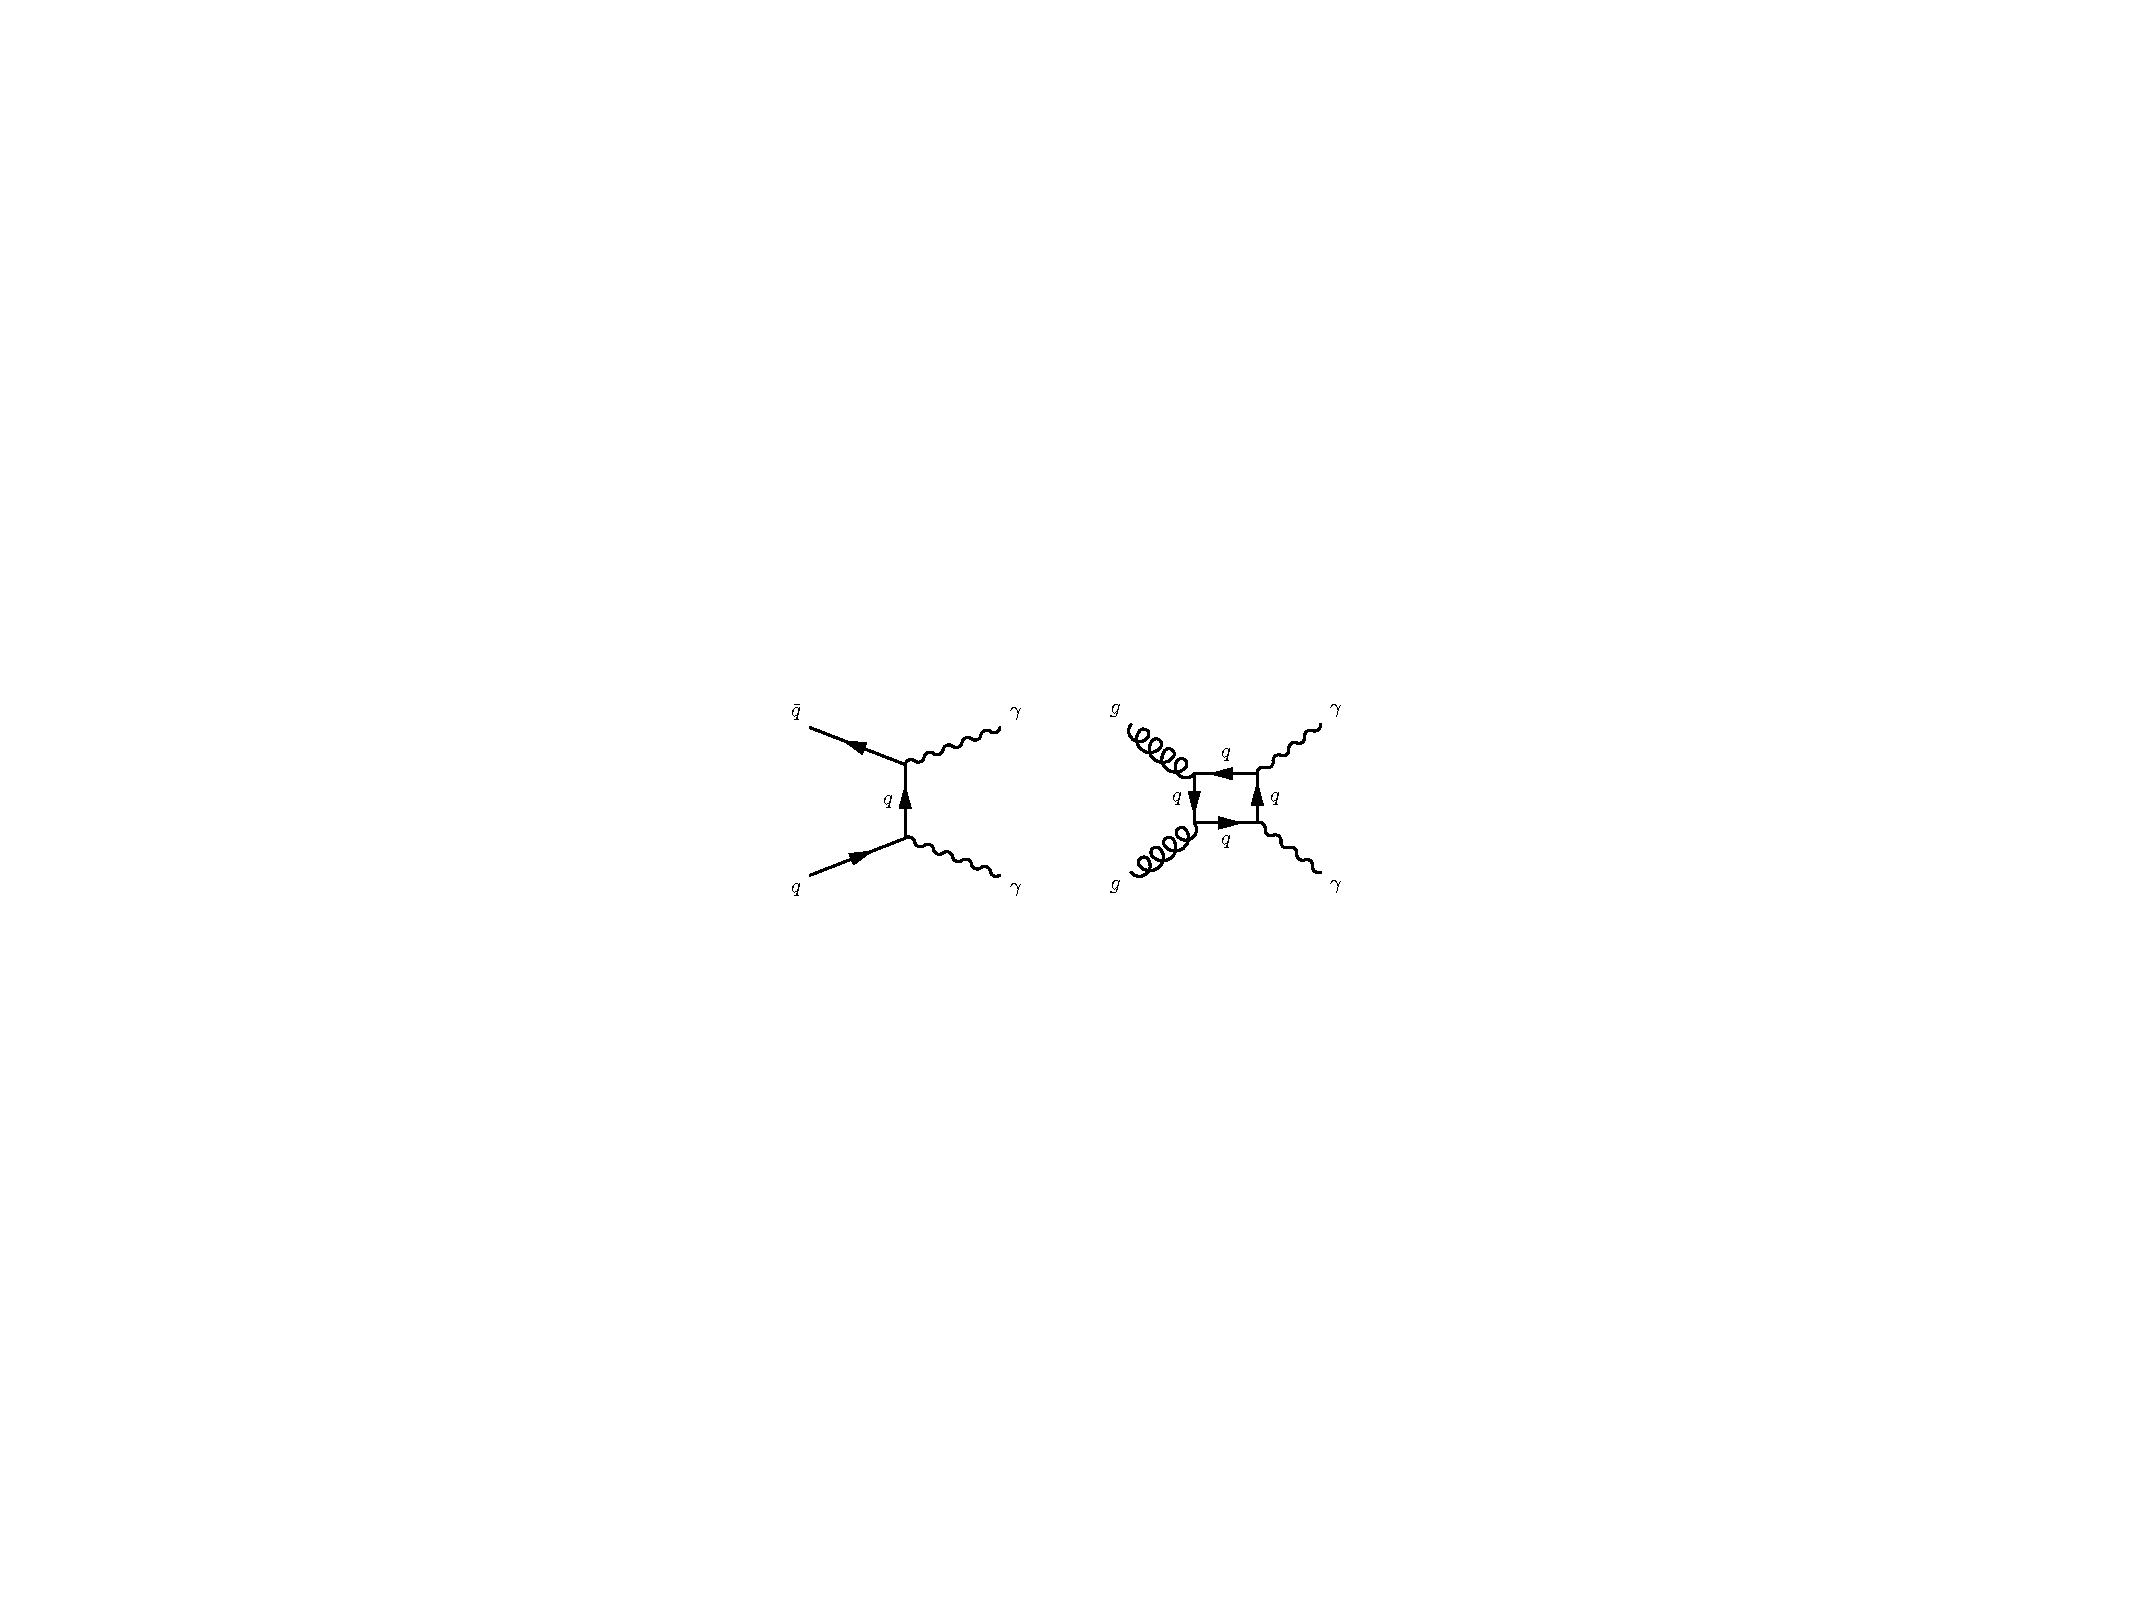
\includegraphics[scale=1.0]{diphoton_cropped}}
	\hspace{1cm}
	\subfloat[$Z\gamma$ production.]{\label{fig:Zgamma}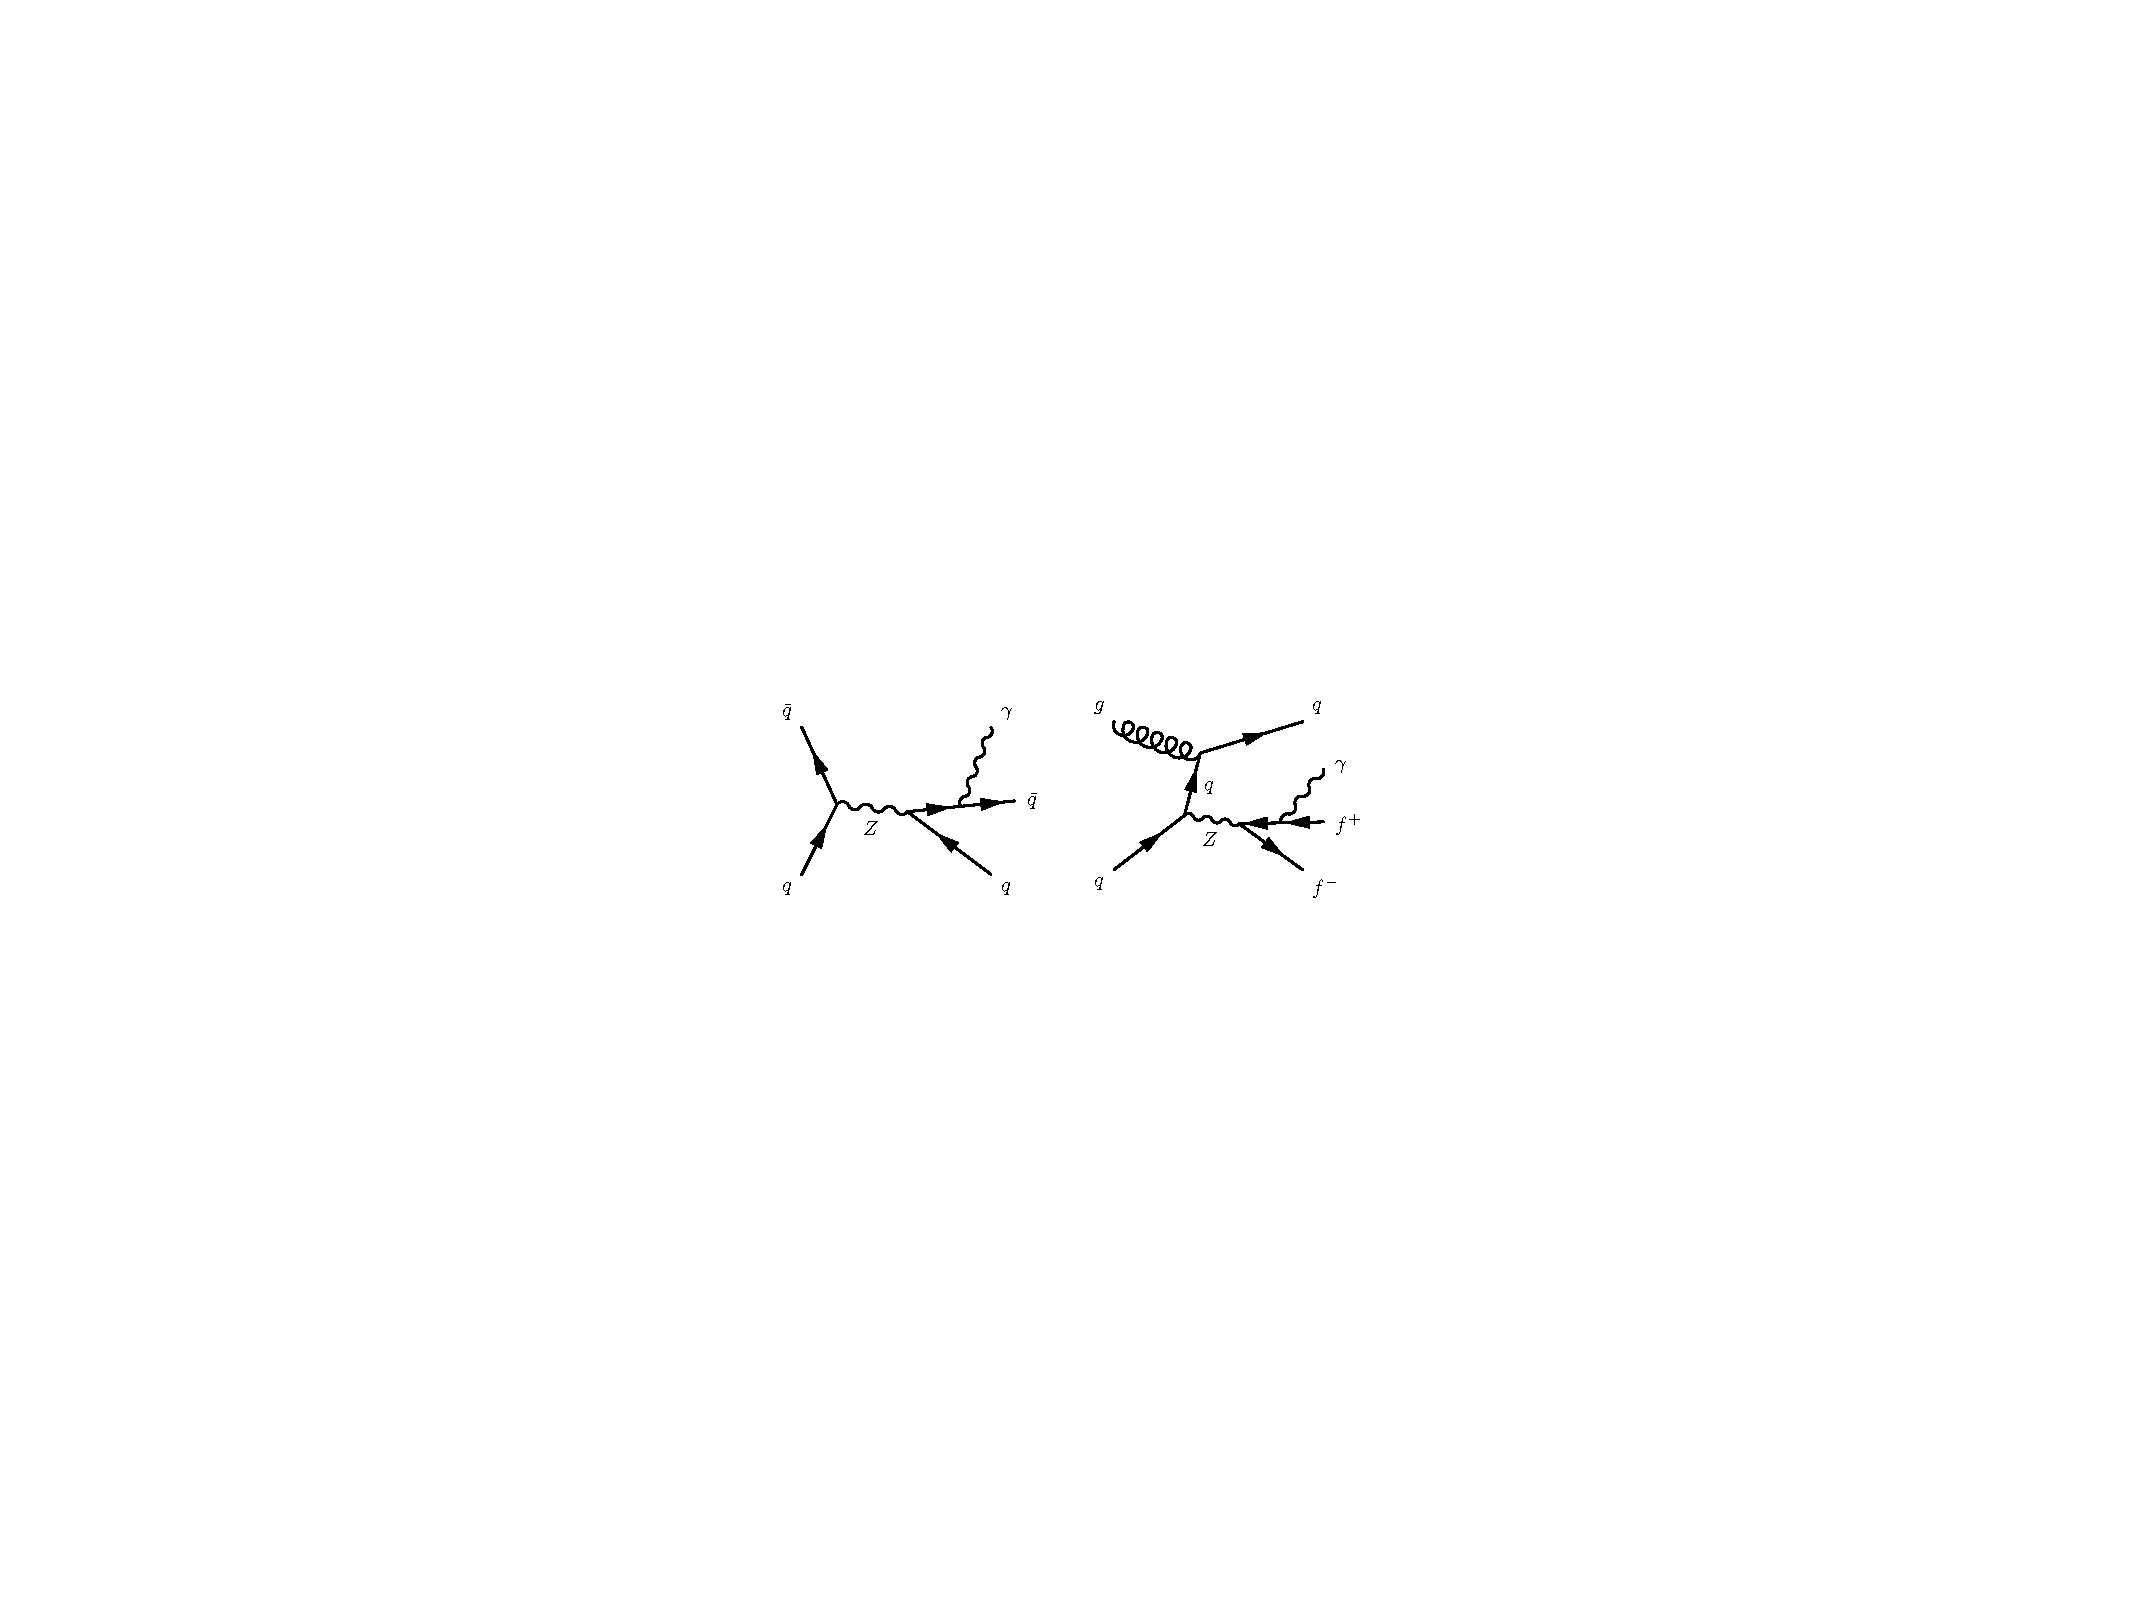
\includegraphics[scale=1.0]{Zgamma_cropped}}
	\caption{Representative Feynman diagrams of some QCD backgrounds to the GGM SUSY search.}
	\label{fig:QCD_background_diagrams}
\end{figure}

\begin{figure}
	\centering
	\subfloat[$W\gamma$ production.]{\label{fig:Wgamma}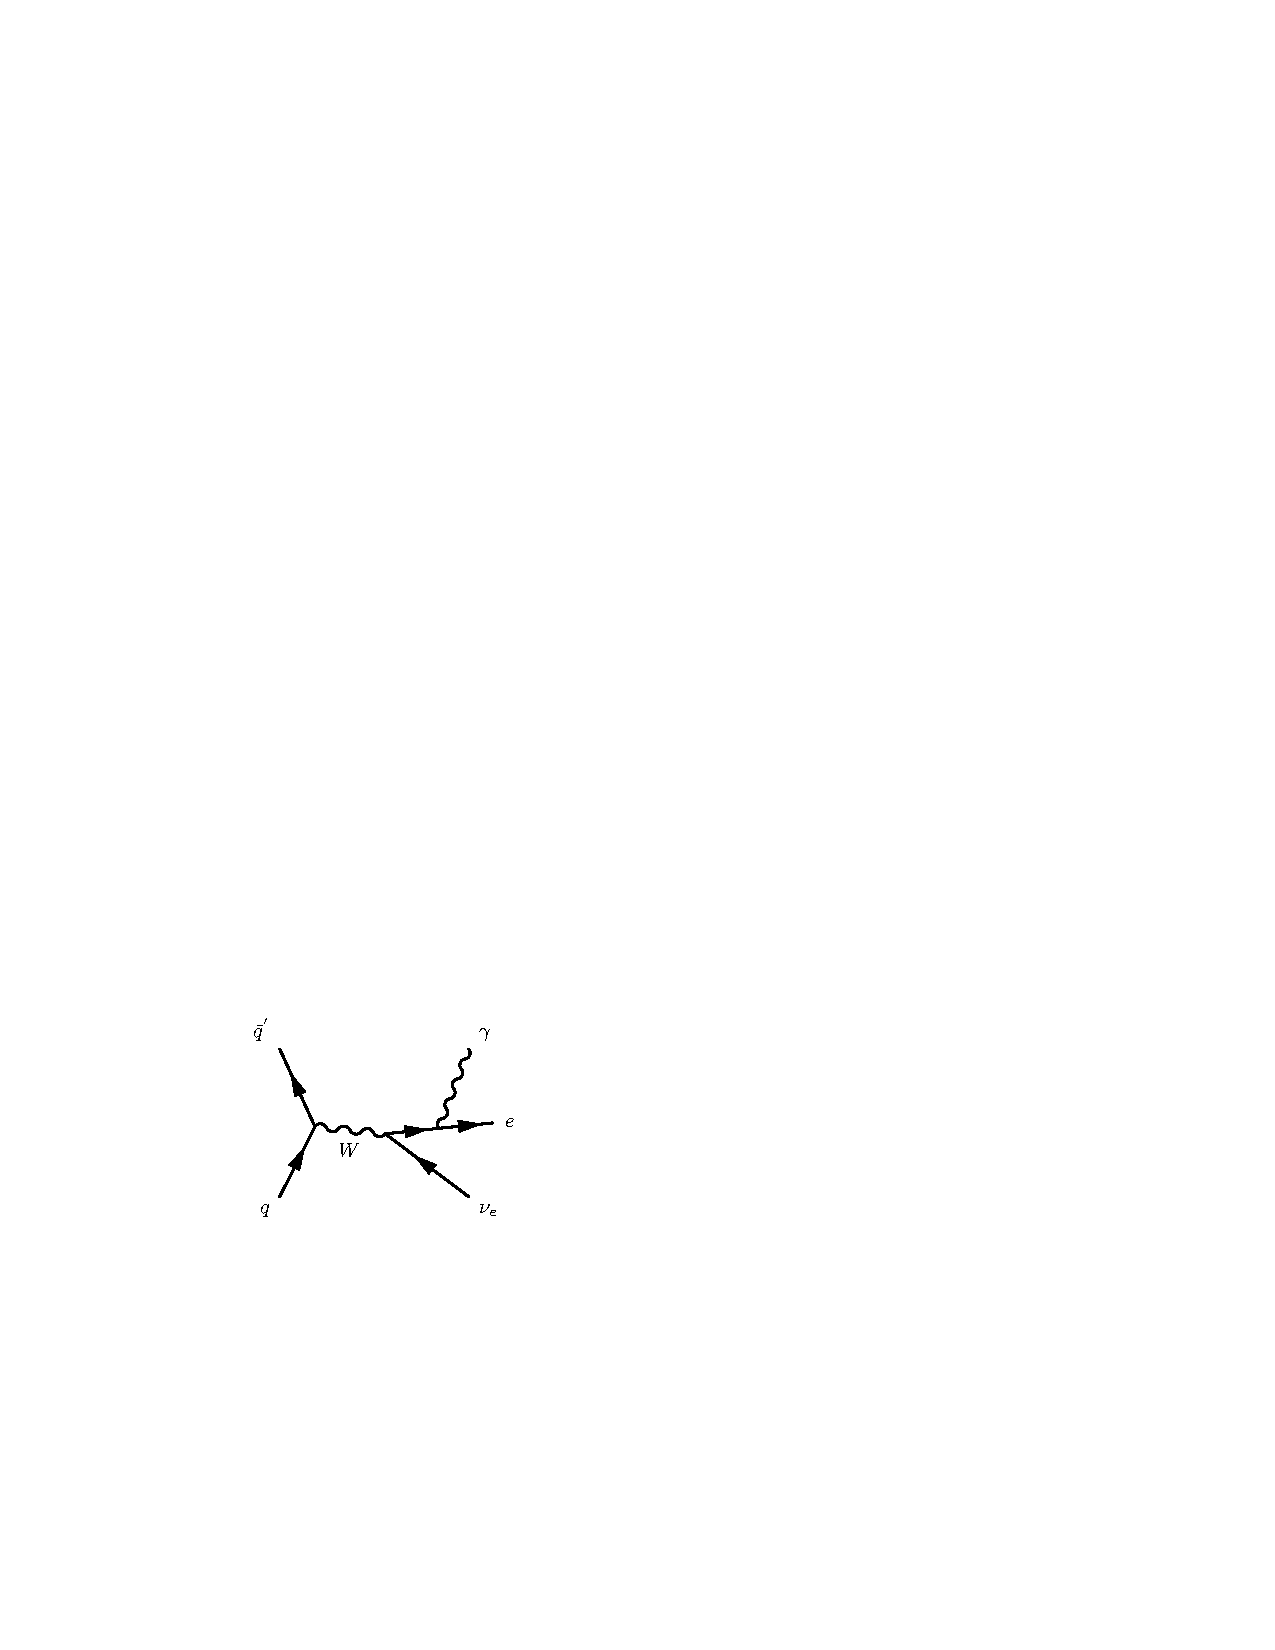
\includegraphics[scale=1.0]{qq_to_W_to_enu_to_enua}}
	\hspace{1cm}
	\subfloat[$W$ + jet production.]{\label{fig:W_jet}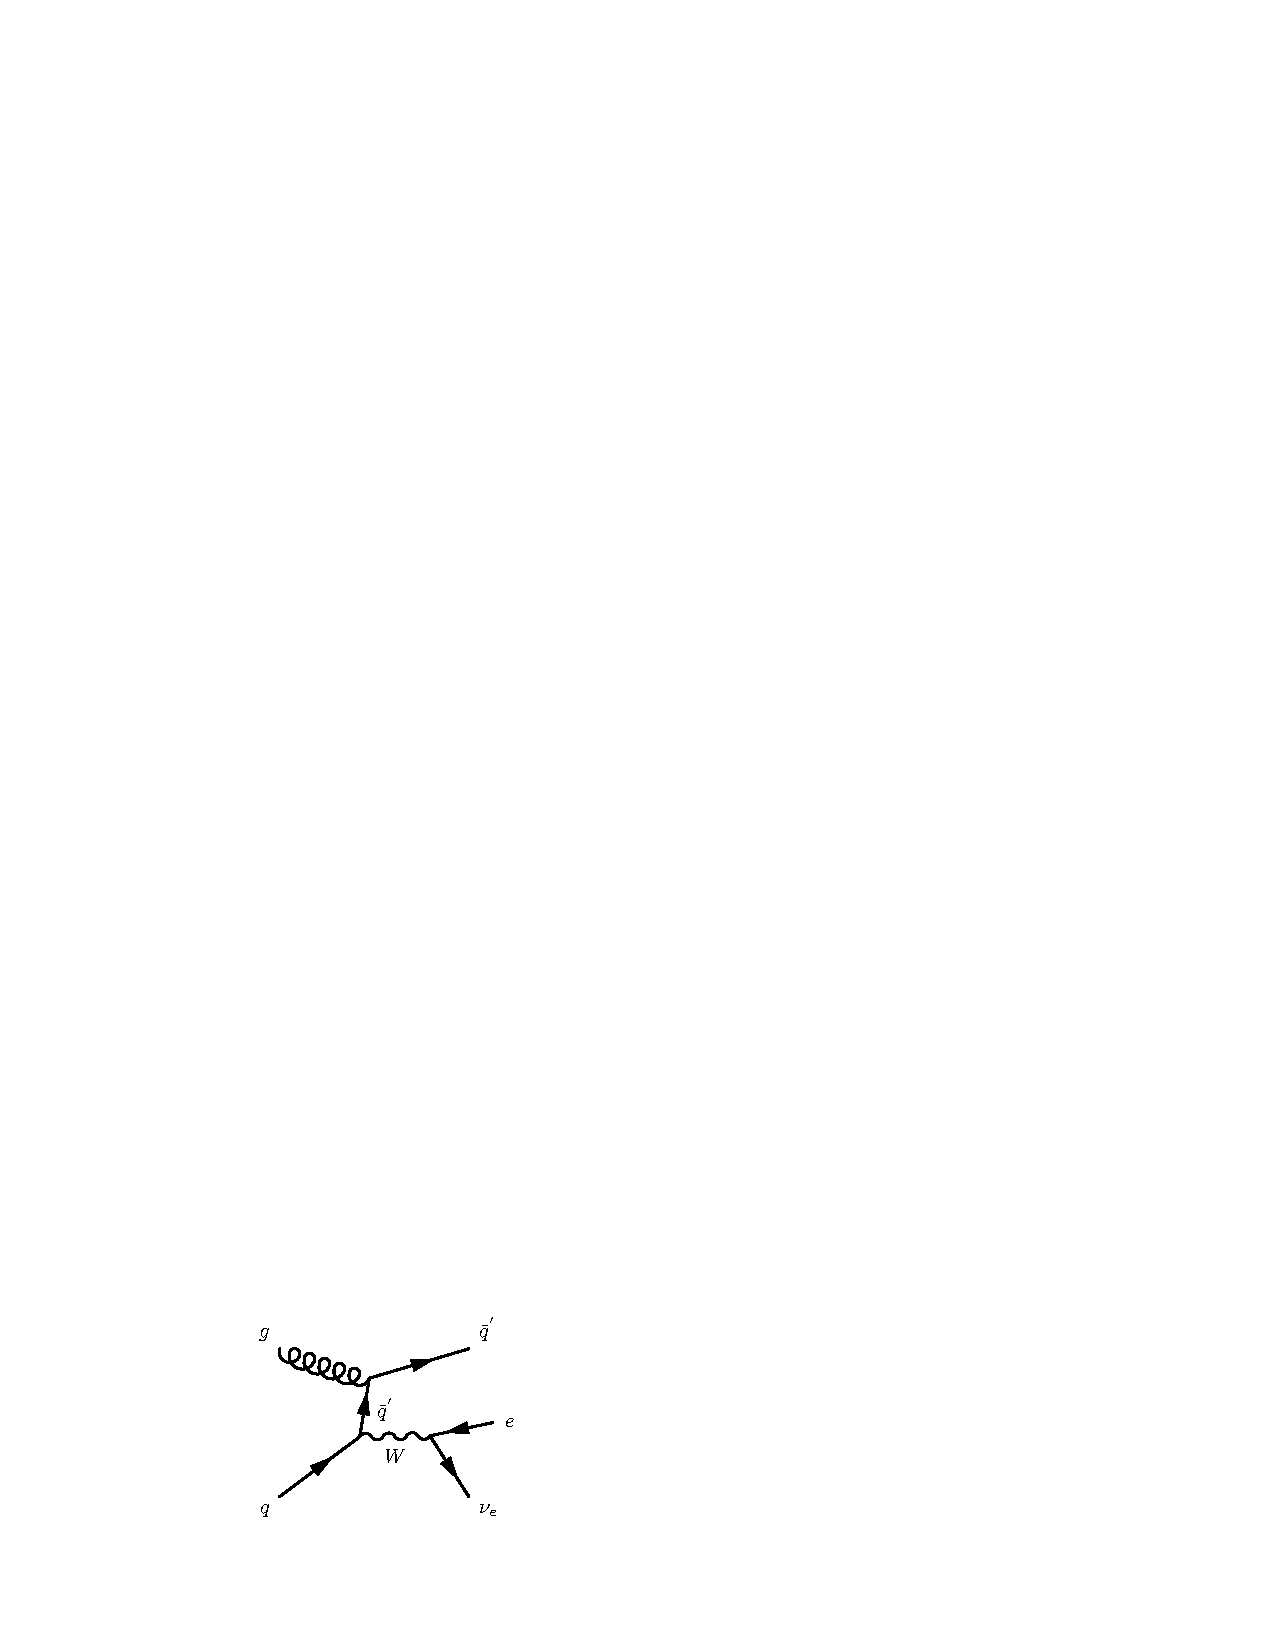
\includegraphics[scale=1.0]{qg_to_qW_to_qenu}}
	\hspace{1cm}
	\subfloat[$t\bar{t}$ production.]{\label{fig:ttbar}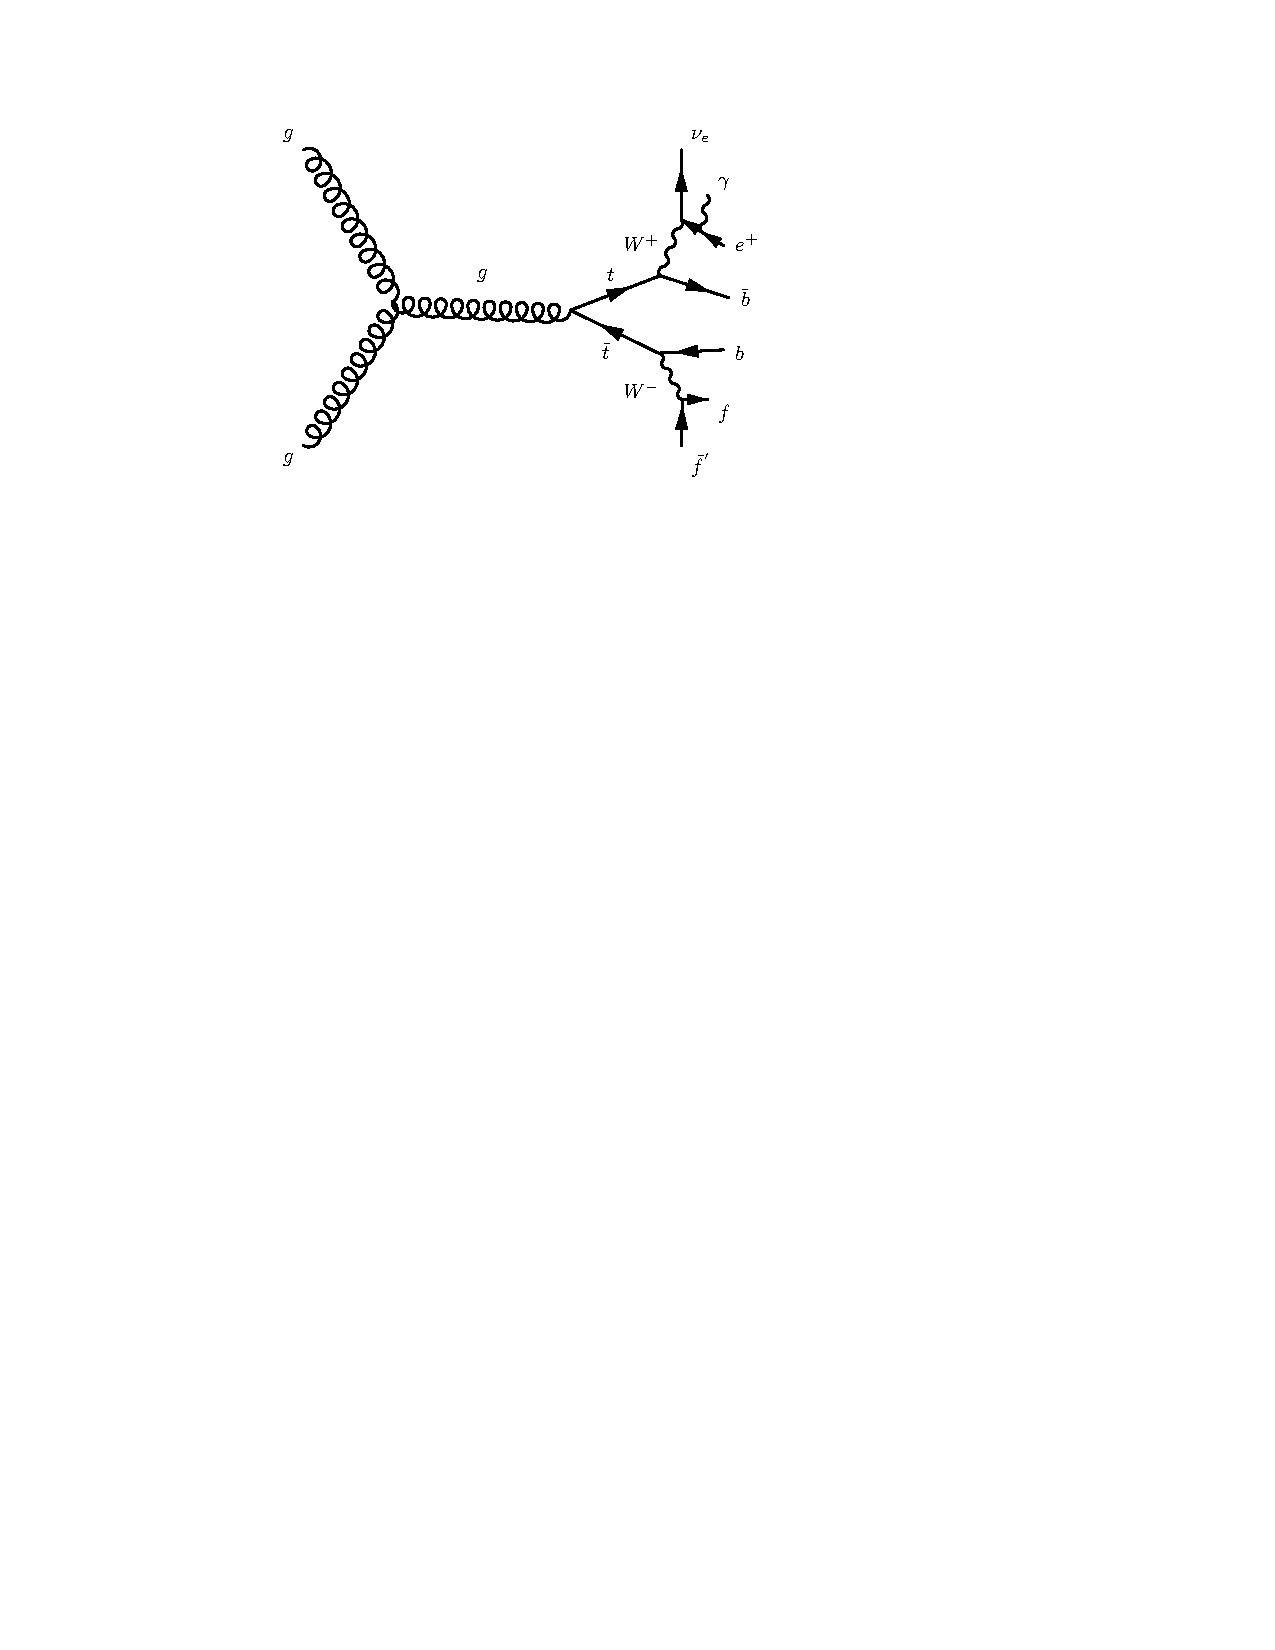
\includegraphics[scale=0.5]{gg_to_tt_to_WbWb_to_ffbenub_to_ffbenuba}}
	\caption{Representative Feynman diagrams of some electroweak backgrounds to the GGM SUSY search.}
	\label{fig:EW_background_diagrams}
\end{figure}

%include a data/MC comparison if time permits
%Figure~\ref{fig:MET_data_vs_MC_backgrounds} shows the \MET spectrum of the $\gamma\gamma$ search data sample overlaid on the \MET spectra of MC simulated background components.  The MC spectra are normalized to the integrated luminosity of the $\gamma\gamma$ data sample.  The dominant background components are QCD inclusive photon processes.  The MC is not used in the actual background estimation.  It is just shown here to illustrate the breakdown of backgrounds.

%\begin{figure}
%	\centering
%	\includegraphics[scale=1.35]{MET_data_vs_MC_backgrounds}
%	\caption{\MET spectrum of the $\gamma\gamma$ search data sample overlaid on the \MET spectra of MC simulated background components.  The MC spectra are normalized to the integrated luminosity of the $\gamma\gamma$ data sample.  A description of the MC samples used may be found in Appendix~\ref{chap:Monte Carlo Samples}}.
%	\label{fig:MET_data_vs_MC_backgrounds}
%\end{figure}

Data control samples are used to model all of the backgrounds.  The primary control sample used to model the QCD background is the $\mathit{ff}$ sample, which is similar to the candidate $\gamma\gamma$ sample but with combined isolation or $\sigma_{i\eta i\eta}$ cuts inverted.  The cuts on these variables are used to distinguish between photons and jets, so by inverting those cuts, the resulting $\mathit{ff}$ sample becomes enriched with QCD dijets.  Because the fake photons are still required to pass a tight cut on $H/E$, they are guaranteed to be very electromagnetic jets, with an EM energy scale and resolution similar to that of the candidate photons.  This insures that the resulting estimate of the \MET shape does not have too long of a tail from severe HCAL mis-measurements that are actually rare in the $\gamma\gamma$ sample.

%append this line to the previous paragraph if time permits
%, as shown in Figure~\ref{fig:MET_MC_ggVsFF_varyHOverE}.  \textcolor{red}{\textbf{Plot the $\gamma\gamma$/$\mathit{ff}$ \MET agreement for different values of the ff $H/E$ cut in MC.  Make the same plot in data for a restricted \MET range?}}

%\begin{figure}
%	\centering
%	\subfloat[MC.  See App.~\ref{chap:Monte Carlo Samples} for the MC samples used.]{\label{fig:MET_MC_ggVsFF_varyHOverE_MC}\includegraphics[scale=1.35]{MET_MC_ggVsFF_varyHOverE_MC}}
%	\hspace{1cm}
%	\subfloat[Data, restricted to $\MET < 100$ GeV.]{\label{fig:MET_MC_ggVsFF_varyHOverE_data}\includegraphics[scale=1.35]{MET_MC_ggVsFF_varyHOverE_data}}
%	\caption{\MET spectra of the $\gamma\gamma$ and $\mathit{ff}$ samples for various values of the $\mathit{ff} H/E$ cut.}
%	\label{fig:MET_MC_ggVsFF_varyHOverE}
%\end{figure}

As a cross-check, the $ee$ sample is also used to model the QCD background.  This sample of $Z$ decays should have no true \MET, just like the $\mathit{ff}$ sample, and the electron definition (differing from the photon definition only in the presence of a pixel seed) insures that the electron energy scale and resolution is similar to that of the photon.

Finally, the $e\gamma$ sample is used to model the electroweak background from $W\rightarrow e\nu$ decays.  The $e\gamma$ \MET distribution is scaled by the electron$\rightarrow$photon misidentification rate to predict the number of $W\gamma$, $W$ + jet, and $t\bar{t}$ events in the $\gamma\gamma$ sample.

The remainder of this chapter describes the data analysis procedures and the final results of the search.  Sec.~\ref{sec:Modeling the QCD Background} addresses the QCD background estimation.  Sec.~\ref{sec:Modeling the Electroweak Background} addresses the electroweak background estimation.  The chapter concludes with a discussion of systematic errors in Sec.~\ref{sec:Errors on the Background Prediction} and a presentation of the final results in Sec.~\ref{sec:Results}.

\section{Modeling the QCD Background}
\label{sec:Modeling the QCD Background}

\subsection{Outline of the Procedure}
\label{sec:Outline of the Procedure}

Due to the fact that the CMS ECAL energy resolution is much better than the HCAL energy resolution, the energies of the two candidate photons in the events of the $\gamma\gamma$ sample are typically measured to far greater accuracy and precision than the energy of the hadronic recoil in those events.  Therefore, fake \MET in the $\gamma\gamma$ sample is almost entirely the result of hadronic mis-measurement in QCD dijet, photon + jet, and diphoton events.  The strategy employed to model this background is to find a control sample in data consisting of two well-measured EM objects, just like the candidate $\gamma\gamma$ sample, and assign each event a weight to account for the underlying kinematic differences between the control and candidate samples.  Once the reweighted \MET spectrum of the control sample is created, it is then normalized in the low-\MET region, the assumption being that GGM SUSY does not predict a significant amount of events at low \MET.  There are three aspects of this QCD background estimation procedure that bear highlighting:

\begin{description}
\item[Choice of control sample] Since the underlying cause of \MET in the candidate sample is mis-measured hadronic activity, a control sample with similar hadronic activity to the candidate sample should be chosen.  Hadronic activity refers to number of jets, jet $E_{T}$, pileup, etc.
\item[Reweighting] The control sample is reweighted so that its \MET spectrum appears as it would if the control sample had the same kinematic properties as the candidate sample (i.e. particle $p_{T}$ and $\eta$ distributions, etc.).  By choosing an appropriate control sample and reweighting it, the control \MET distribution should now match both the hadronic activity and the kinematics of the candidate sample.
\item[Normalization] Finally, the control \MET distribution is normalized in a region of low \MET, where contamination from the expected GGM SUSY signal is small.  This implies an extrapolation of the low-\MET QCD background prediction to the high-\MET signal region.
\end{description}

As explained in the beginning of this chapter, the $\mathit{ff}$ sample is used as the primary QCD control sample, while the $ee$ sample is used as a cross-check.  Both samples have two well-measured EM objects per event, no real \MET, and similar hadronic activity to the $\gamma\gamma$ sample.  Figure~\ref{fig:hadronic_activity} shows a comparison of the shapes of some distributions relevant to hadronic activity between the $\gamma\gamma$, $ee$, and $\mathit{ff}$ samples.  In general, the $ee$ sample has less hadronic activity than the $\gamma\gamma$ and $\mathit{ff}$ samples, as shown by the more steeply falling $ee$ distributions in Figs.~\ref{fig:hadronic_activity_HT},~\ref{fig:hadronic_activity_Nj},~\ref{fig:hadronic_activity_MHT}, and~\ref{fig:hadronic_activity_j1ET}.  In addition to the kinematic reweighting, there is also a reweighting by number of jets per event, which attempts to correct for this difference (see Sec.~\ref{sec:Reweighting}).

\begin{figure}
	\centering
	\subfloat[$H_{T}$, defined as the scalar sum of corrected jet $E_{T}$ for jets defined as in Table~\ref{tab:jet_definition}.]{\label{fig:hadronic_activity_HT}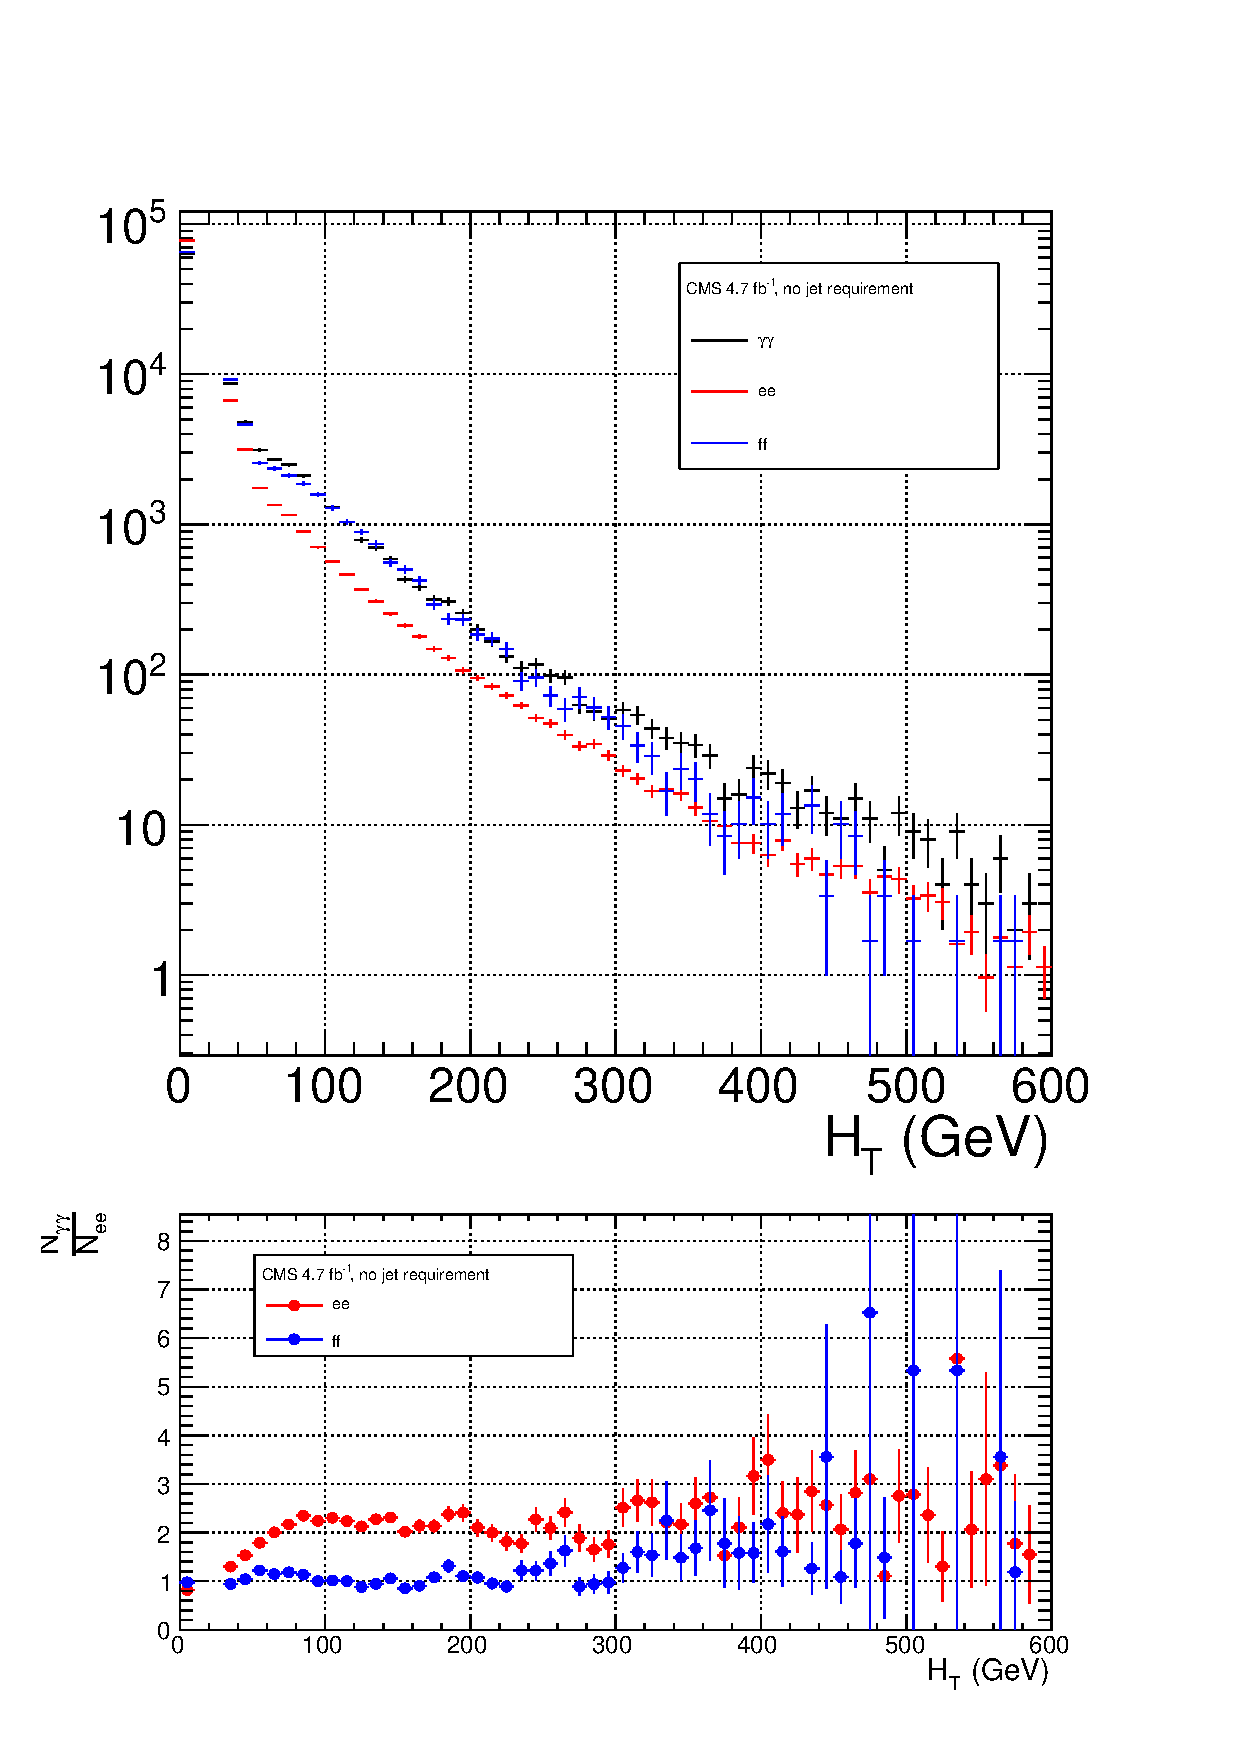
\includegraphics[scale=0.25]{hadronic_activity_HT}}
	\hspace{0.75cm}
	\subfloat[Number of jets per event for jets defined as in Table~\ref{tab:jet_definition}.]{\label{fig:hadronic_activity_Nj}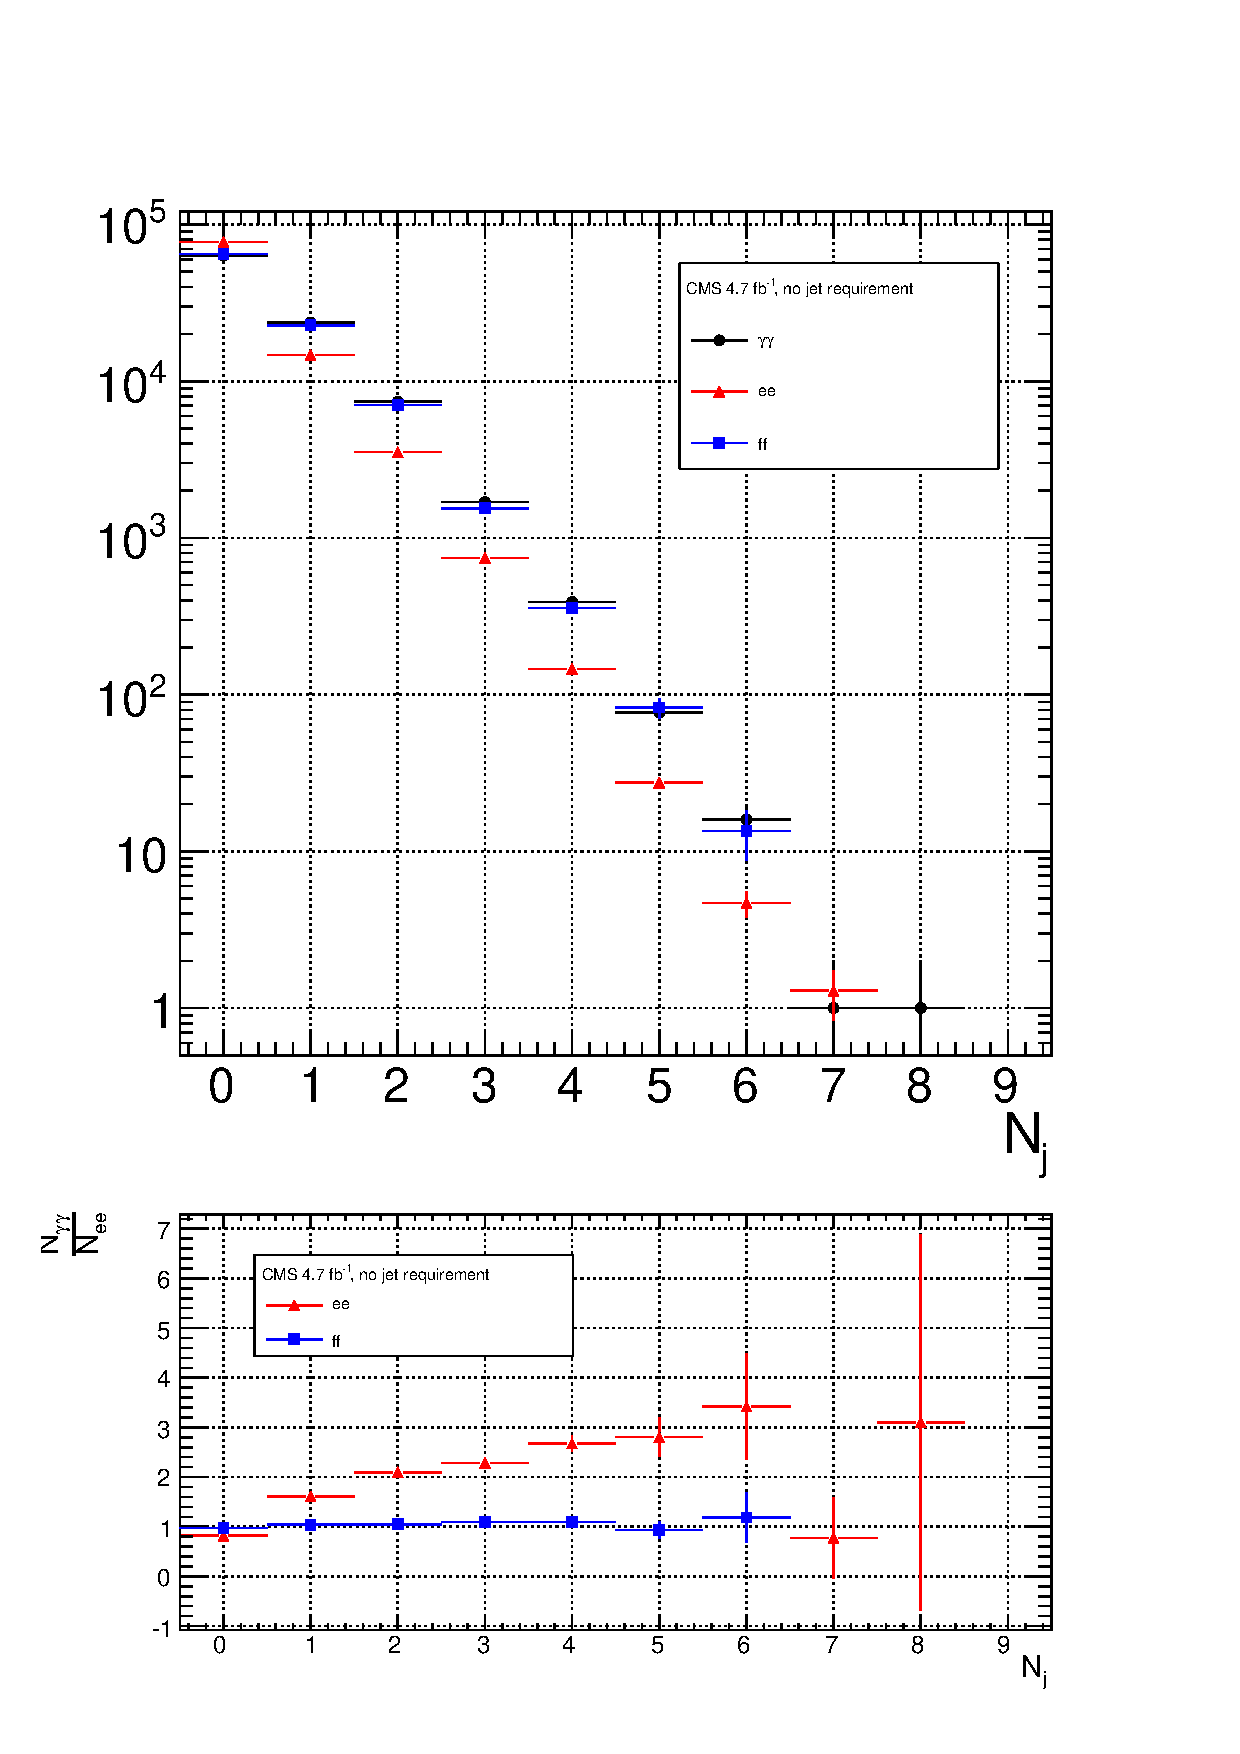
\includegraphics[scale=0.25]{hadronic_activity_Nj}}
	\hspace{0.75cm}
	\subfloat[$\not\!\! H_{T}$, defined as the magnitude of the negative vectorial sum of corrected jet $E_{T}$ for jets defined as in Table~\ref{tab:jet_definition}.]{\label{fig:hadronic_activity_MHT}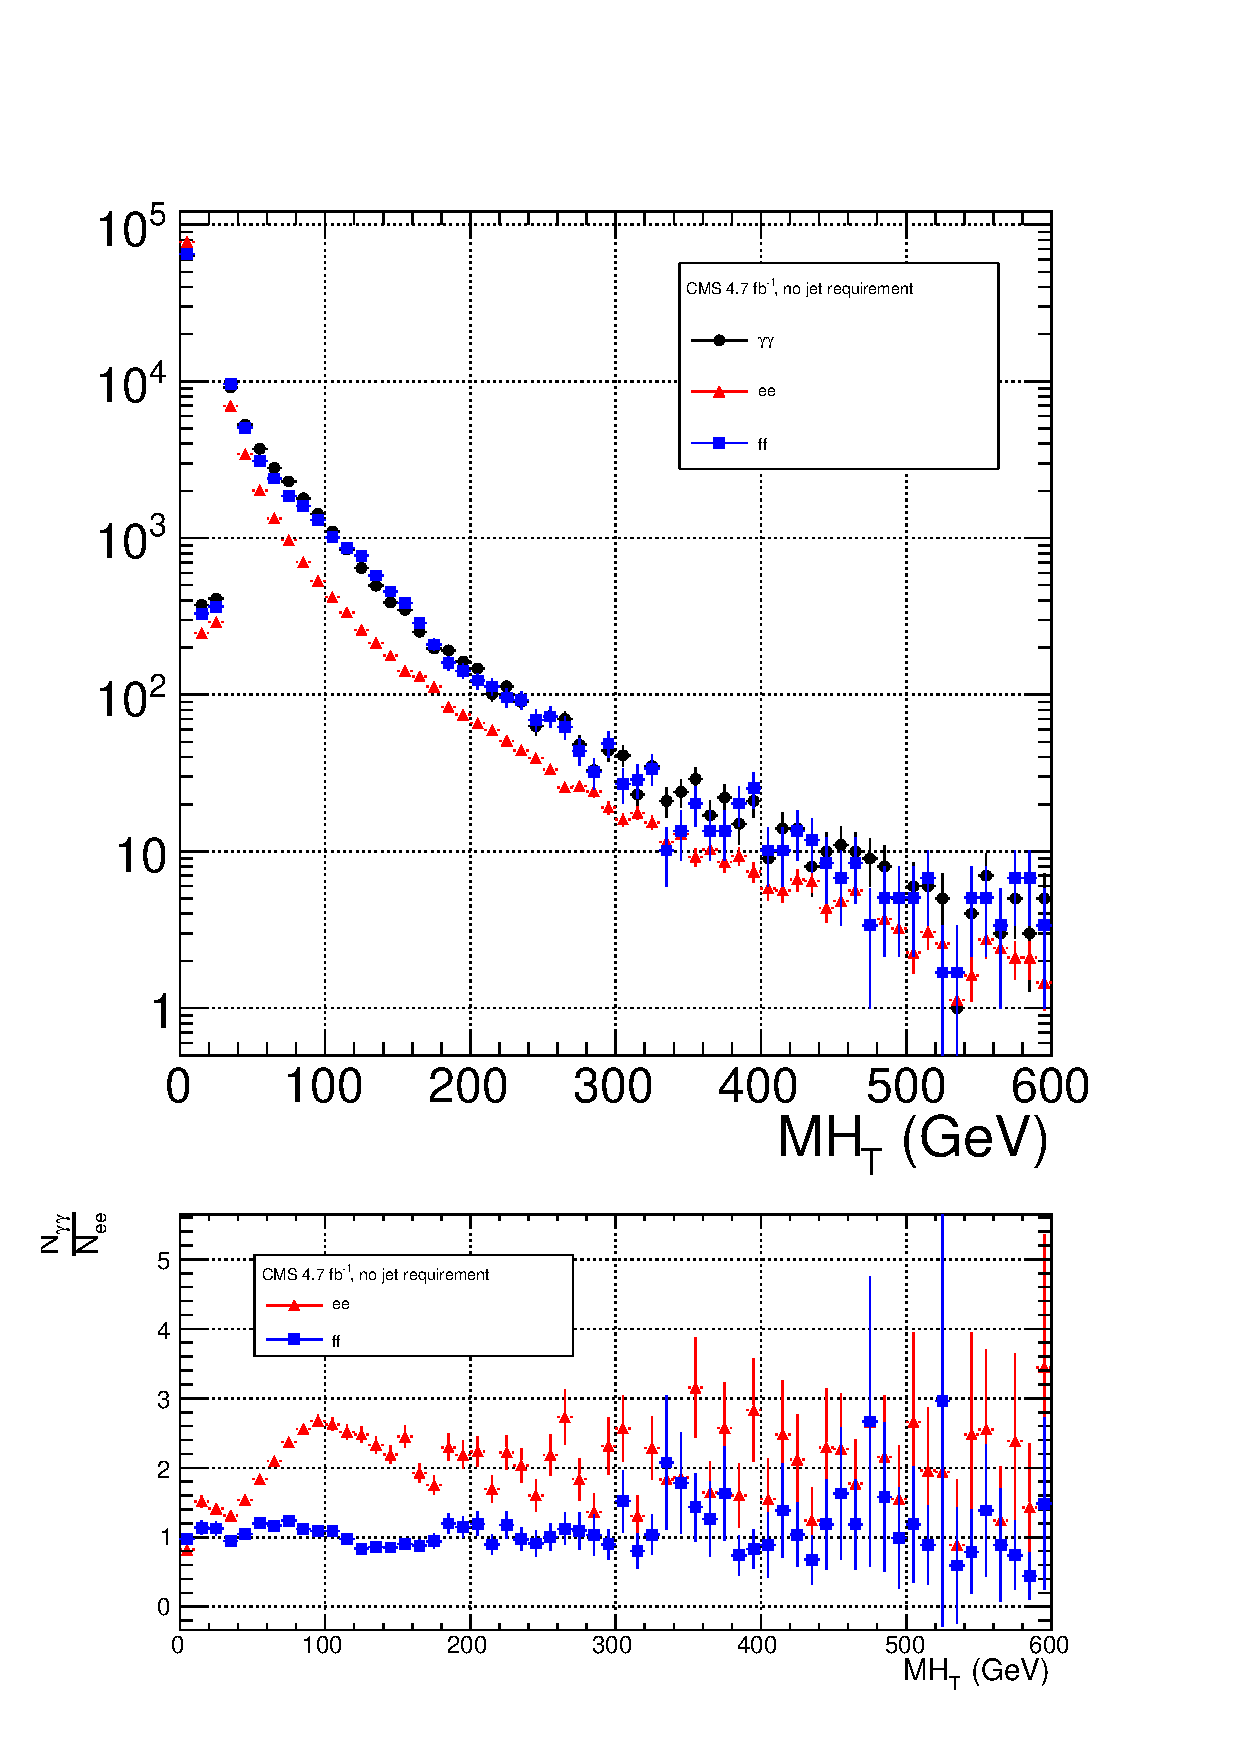
\includegraphics[scale=0.25]{hadronic_activity_MHT}}
	\\
	\subfloat[Corrected $E_{T}$ for the jet with the largest corrected $E_{T}$ per event, for jets defined as in Table~\ref{tab:jet_definition} (excluding the $p_{T}$ requirement).]{\label{fig:hadronic_activity_j1ET}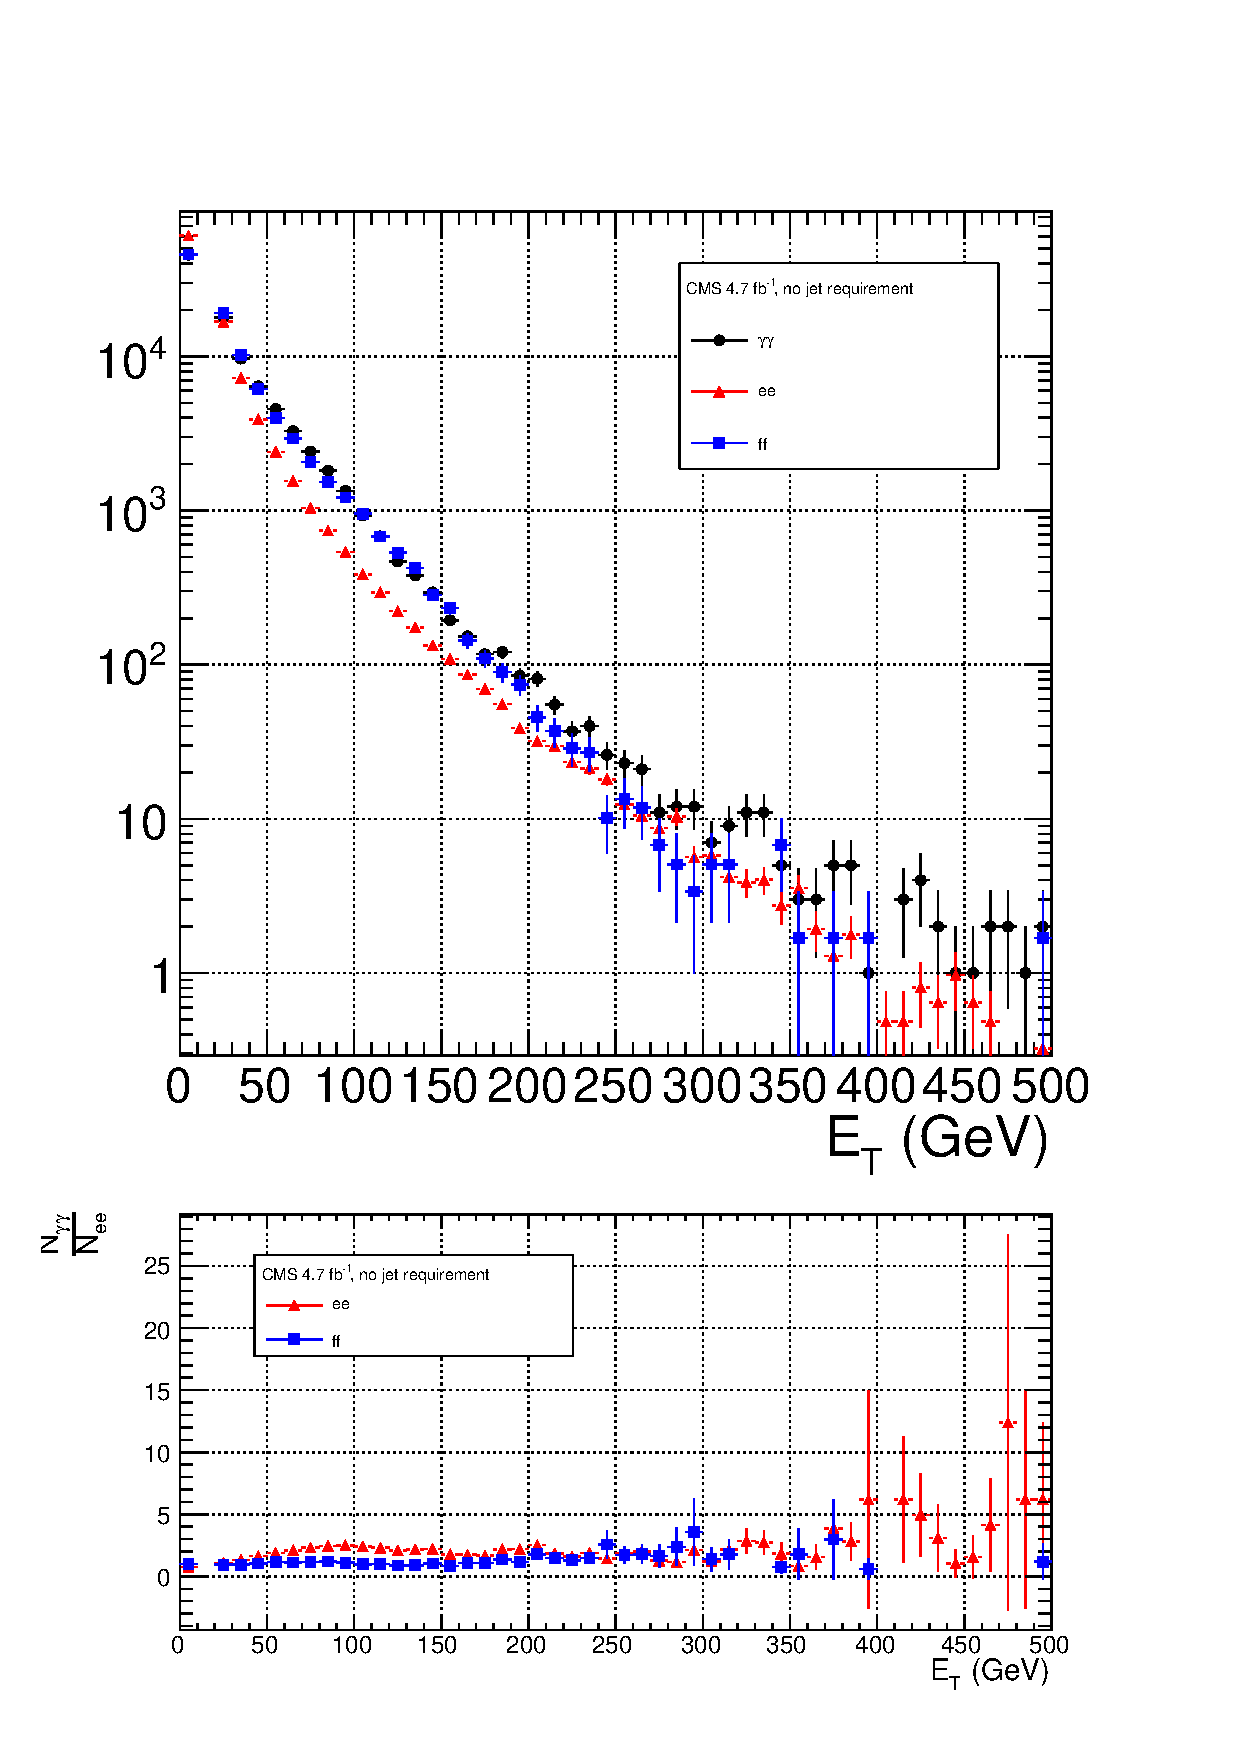
\includegraphics[scale=0.25]{hadronic_activity_j1ET}}
	\hspace{0.75cm}
	\subfloat[$\rho$ (average pileup energy density in the calorimeters per unit $\eta\cdot\phi$, cf. Sec.~\ref{sec:Photons}).]{\label{fig:hadronic_activity_rho}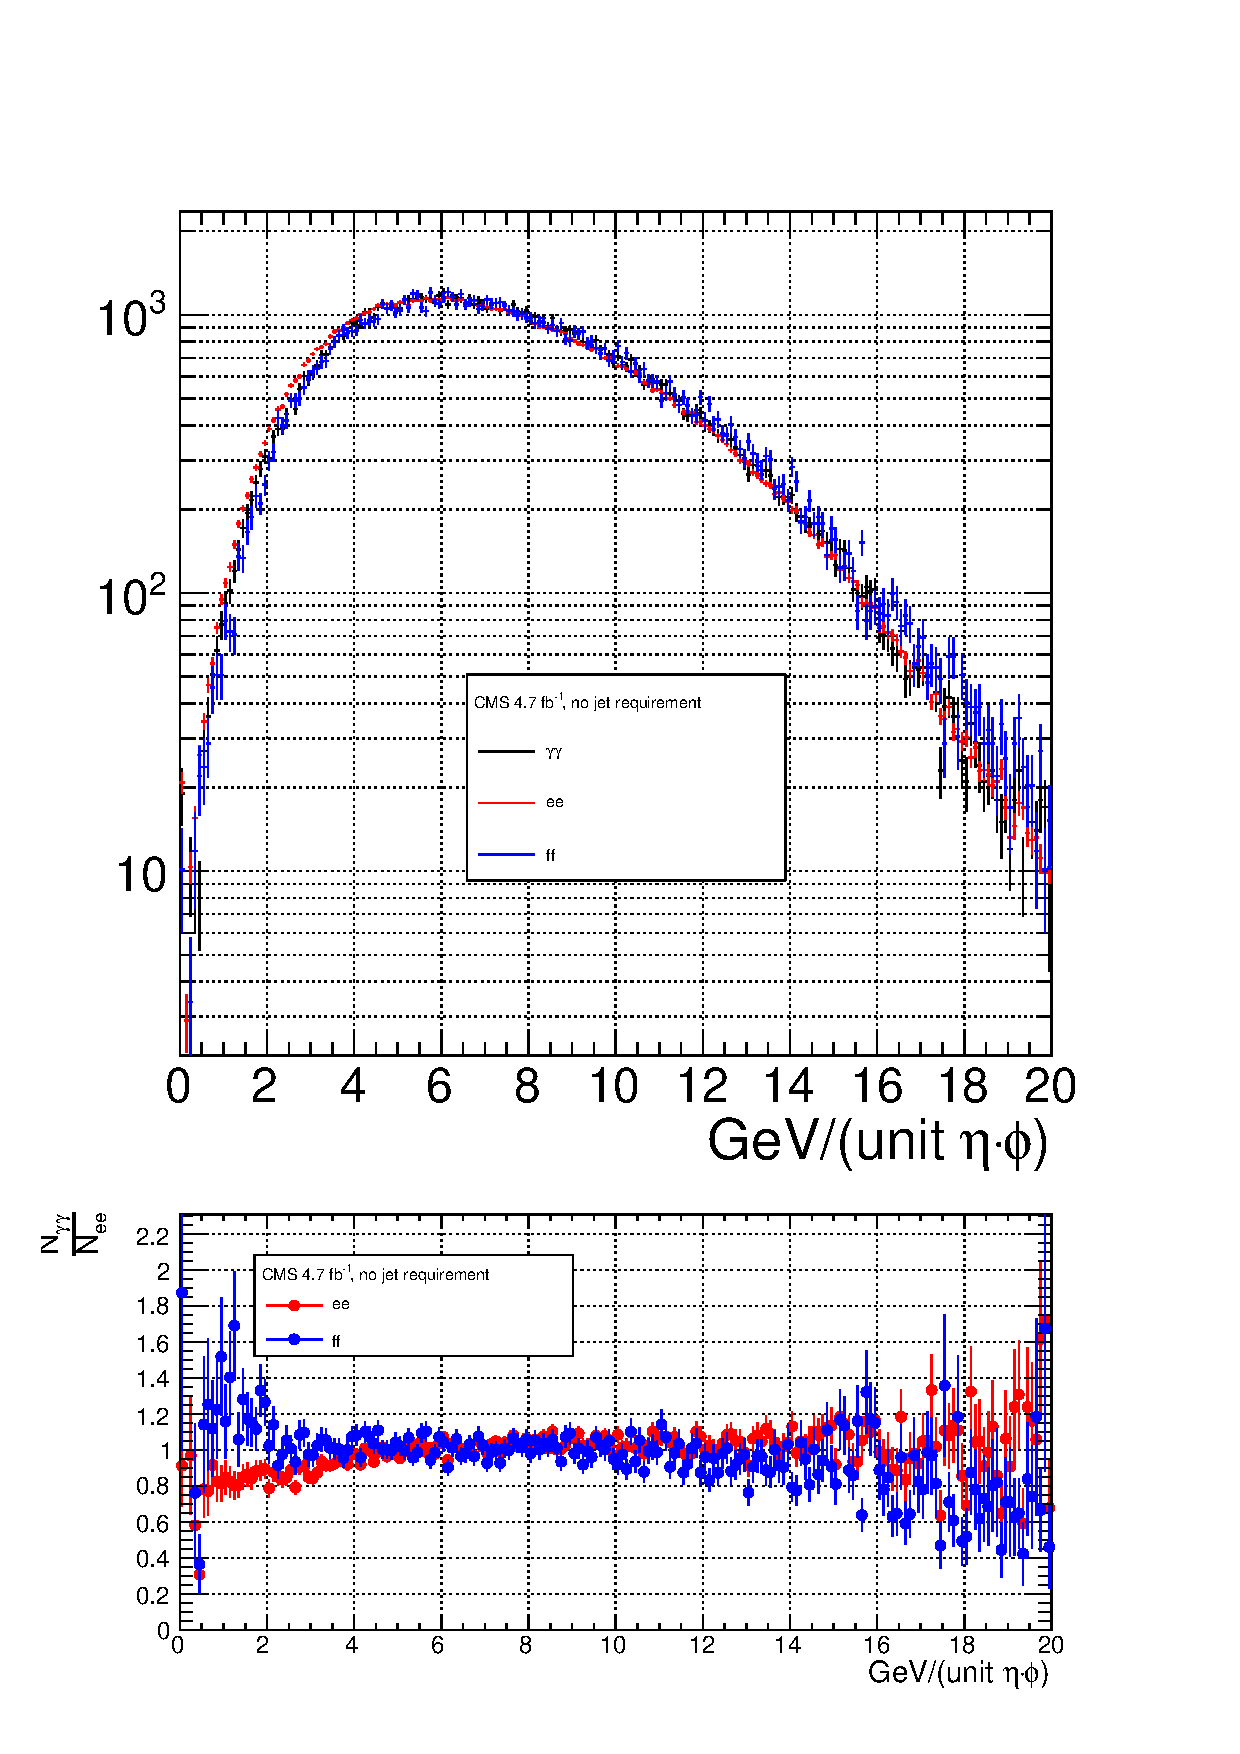
\includegraphics[scale=0.25]{hadronic_activity_rho}}
	\hspace{0.75cm}
	\subfloat[Number of good reconstructed primary vertices per event according to the criteria of Sec.~\ref{sec:Event Quality}.]{\label{fig:hadronic_activity_nPV}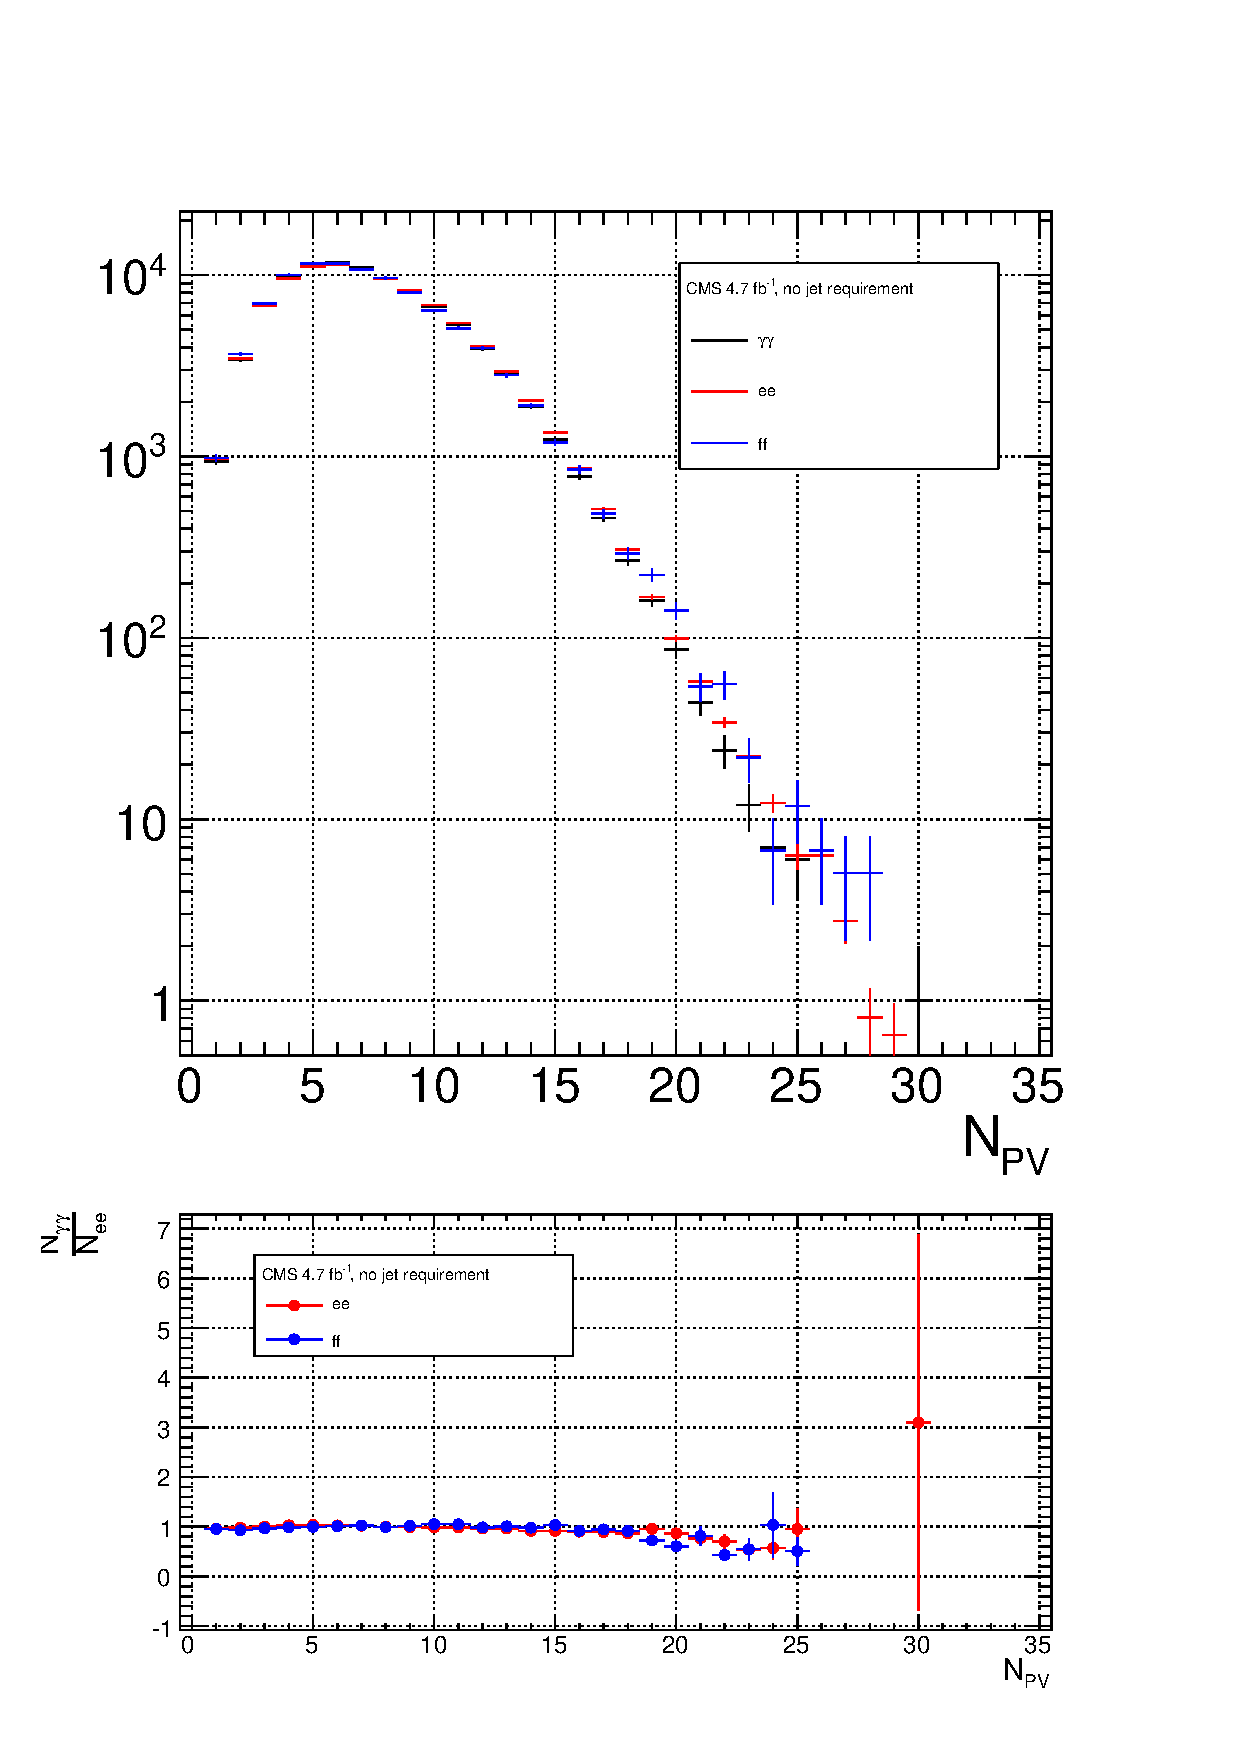
\includegraphics[scale=0.25]{hadronic_activity_nPV}}
	\caption{Comparison of the shapes of some distributions relevant to hadronic activity between the $\gamma\gamma$, $ee$ (81 GeV $\leq m_{\mathrm{ee}} <$ 101 GeV), and $\mathit{ff}$ samples.  The $ee$ and $\mathit{ff}$ distributions are normalized to the number of events in the $\gamma\gamma$ distribution.  Errors are statistical only.}
	\label{fig:hadronic_activity}
\end{figure}

\begin{table}[hcbp]
\caption{Definition of HB/HE/HF hadronic jets.}
\centering
\begin{minipage}{\textwidth}
\centering
\begin{tabular}{|c|c|}
\hline
Variable & Cut \\
\hline
\hline
Algorithm & \verb+L1FastL2L3Residual+ corrected PF (cf. Sec.~\ref{sec:Jets and Missing Transverse Energy}) \\
\hline
$p_{T}$ & $> 30$ GeV \\
\hline
$|\eta|$ & $< 5.0$ \\
\hline
\begin{tabular}[c]{@{}c@{}}Neutral hadronic\\energy fraction\end{tabular} & $< 0.99$ \\
\hline
\begin{tabular}[c]{@{}c@{}}Neutral electromagnetic\\energy fraction\end{tabular} & $< 0.99$ \\
\hline
Number of constituents & $> 1$ \\
\hline
Charged hadronic energy & $> 0.0$ GeV if $|\eta|  < 2.4$ \\
\hline
Number of charged hadrons & $> 0$ if $|\eta|  < 2.4$ \\
\hline
\begin{tabular}[c]{@{}c@{}}Charged electromagnetic\\energy fraction\end{tabular} & $< 0.99$ if $|\eta| < 2.4$ \\
\hline
\begin{tabular}[c]{@{}c@{}}$\Delta R$ to nearest PF electron\footnote{A PF electron is defined as an electron reconstructed with the PF algorithm \cite{CMS_AN-2010/034} with $p_{T} >$ 15 GeV, $|\eta| <$ 2.6, and ($I_{\mathrm{charged}} + I_{\mathrm{photon}} + I_{\mathrm{neutral}}$)/$p_{T} <$ 0.2, where $I_{\mathrm{charged}}$($I_{\mathrm{photon}}$)($I_{\mathrm{neutral}}$) is the sum of PF charged hadron(PF photon)(PF neutral hadron) momenta in a $\Delta$R = 0.4 cone around the PF electron.}, muon\footnote{Muons are reconstructed \cite{CMS_CR-2009/347} from a combination of muon station and inner tracker hits.  Here, a muon must have track $\chi^{2} <$ 10, at least one good muon station hit, inner track transverse impact parameter $<$ 0.02 cm, inner track longitudinal impact parameter $<$ 0.5 cm, $p_{T} >$ 15 GeV, $|\eta| <$ 2.6, and ($I_{\mathrm{ECAL}} + I_{\mathrm{HCAL}} + I_{\mathrm{track}}$)/$p_{T} <$ 0.2, where $I_{\mathrm{ECAL}}$($I_{\mathrm{HCAL}}$)($I_{\mathrm{track}}$) is the sum of ECAL(HCAL)(track) momenta in a $\Delta$R = 0.3 cone around the muon.},\\or one of the two\\primary EM objects\end{tabular} & $> 0.5$ \\
\hline
\end{tabular}
\end{minipage}
\label{tab:jet_definition}
\end{table}

\subsection{Reweighting}
\label{sec:Reweighting}

To reweight the control sample events to match the kinematics of the candidate sample events, a weight based on the $p_{T}$ of the di-EM-object system and the number of jets in the event is used.  As explained in Sec.~\ref{sec:Outline of the Procedure}, \MET in the $\gamma\gamma$, $\mathit{ff}$, and $ee$ samples is due to the poorly measured hadronic recoil off the well-measured di-EM system.  Therefore, the $p_{T}$ of the di-EM system is a good handle on the true magnitude of the hadronic recoil, which affects the measured \MET.  The di-EM system is depicted in Figure~\ref{fig:di-EM_pT_cartoon}.  As shown in Figure~\ref{fig:MET_vs_di-EM_pT}, \MET is largely uncorrelated with di-EM $p_{T}$, so there is little danger of reweighting away a true signal excess.

\begin{figure}
	\centering
	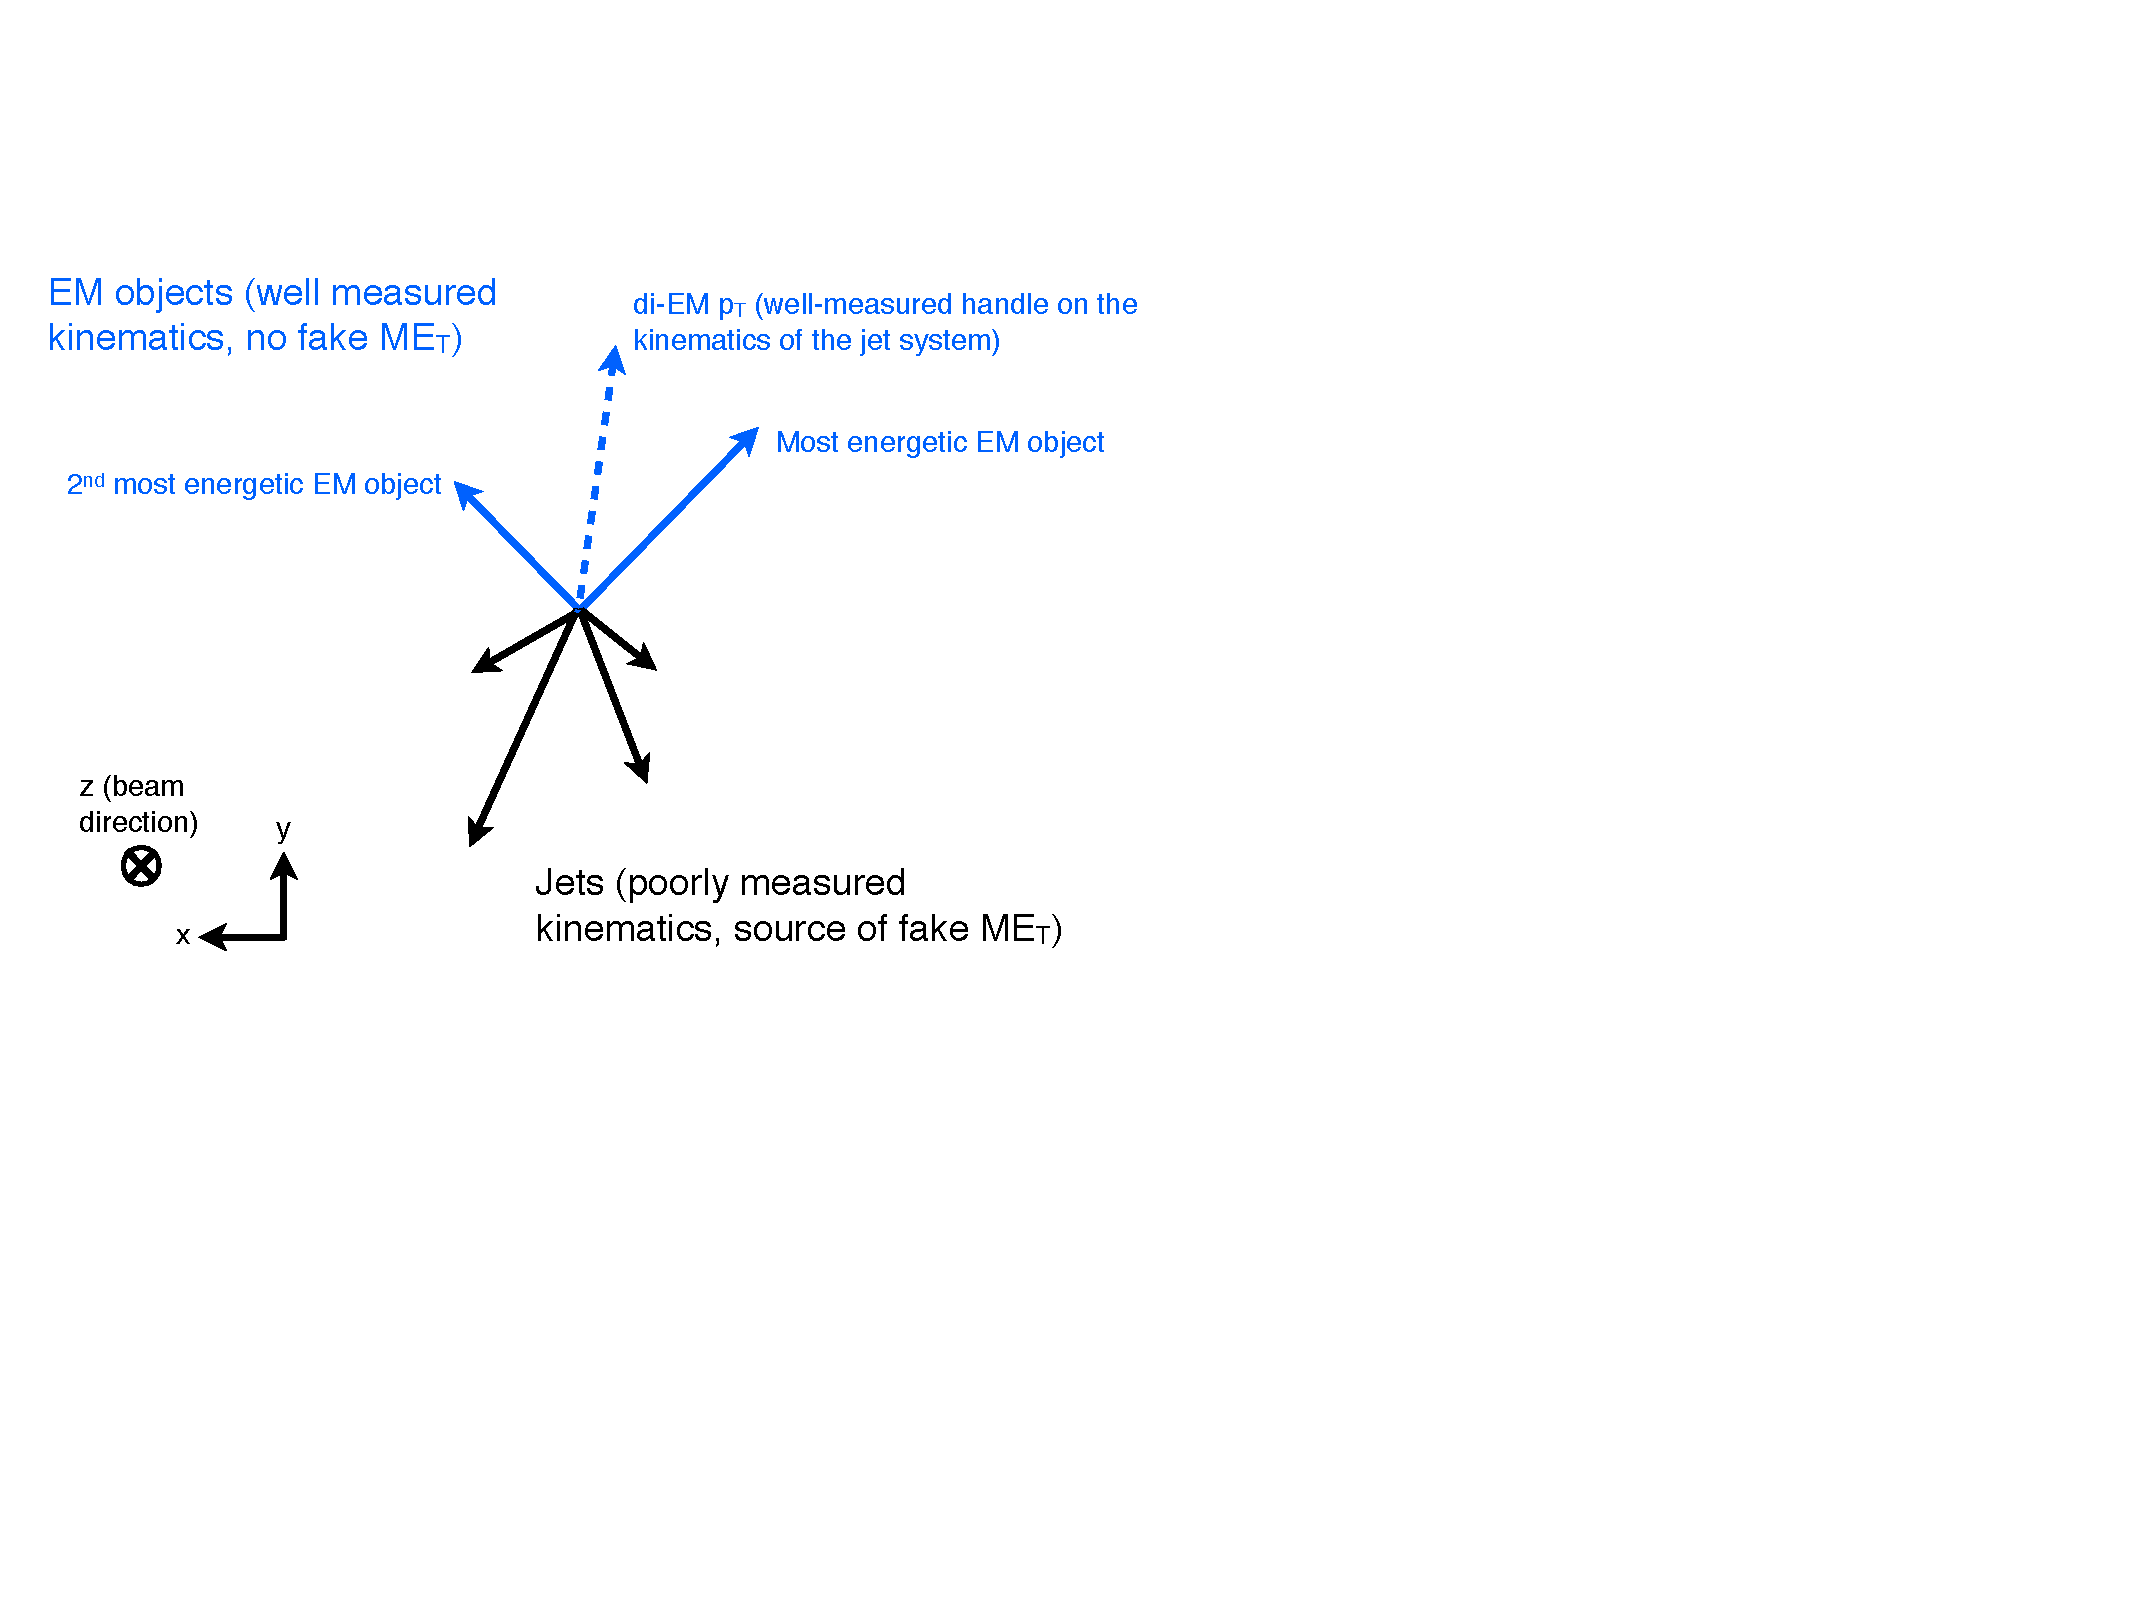
\includegraphics[scale=0.5]{di-EM_pT_cartoon}
	\caption{Cartoon showing the di-EM system in blue and the hadronic recoil in black.  The di-EM $p_{T}$ (dashed blue line) is used to reweight the control sample kinematic properties to match those of the candidate $\gamma\gamma$ sample.}.
	\label{fig:di-EM_pT_cartoon}
\end{figure}

\begin{figure}
	\centering
	\subfloat[$\gamma\gamma$.]{\label{fig:gg_MET_vs_di-EM_pT}\includegraphics[scale=0.2]{gg_MET_vs_di-EM_pT}}
	\hspace{1cm}
	\subfloat[$ee$.]{\label{fig:ee_MET_vs_di-EM_pT}\includegraphics[scale=0.2]{ee_MET_vs_di-EM_pT}}
	\hspace{1cm}
	\subfloat[$\mathit{ff}$.]{\label{fig:ff_MET_vs_di-EM_pT}\includegraphics[scale=0.2]{ff_MET_vs_di-EM_pT}}
	\caption{\MET vs. di-EM $p_{T}$.}
	\label{fig:MET_vs_di-EM_pT}
\end{figure}

Whereas the di-EM $p_{T}$ reweighting accounts for differences in production kinematics between the control and $\gamma\gamma$ samples, a simultaneous reweighting based on the number of jets in the event accounts for differences in hadronic activity between the samples, especially between $ee$ and $\gamma\gamma$ (cf. Fig.~\ref{fig:hadronic_activity}).  Jets are defined as in Table~\ref{tab:jet_definition_for_Nj_reweighting}.  Figure~\ref{fig:dijet_pT_and_Nj_vs_dijet_pT_reweighting} shows the effect of reweighting by number of jets per event, which is to increase(decrease) the tail of the $ee$($\mathit{ff}$) \MET spectrum.

%include ee/gg and ff/gg agreement?
%include similar figures for MC?
\begin{figure}
	\centering
	\subfloat[$ee$ \MET spectra.]{\label{fig:ee_dijet_pT_and_Nj_vs_dijet_pT_reweighting}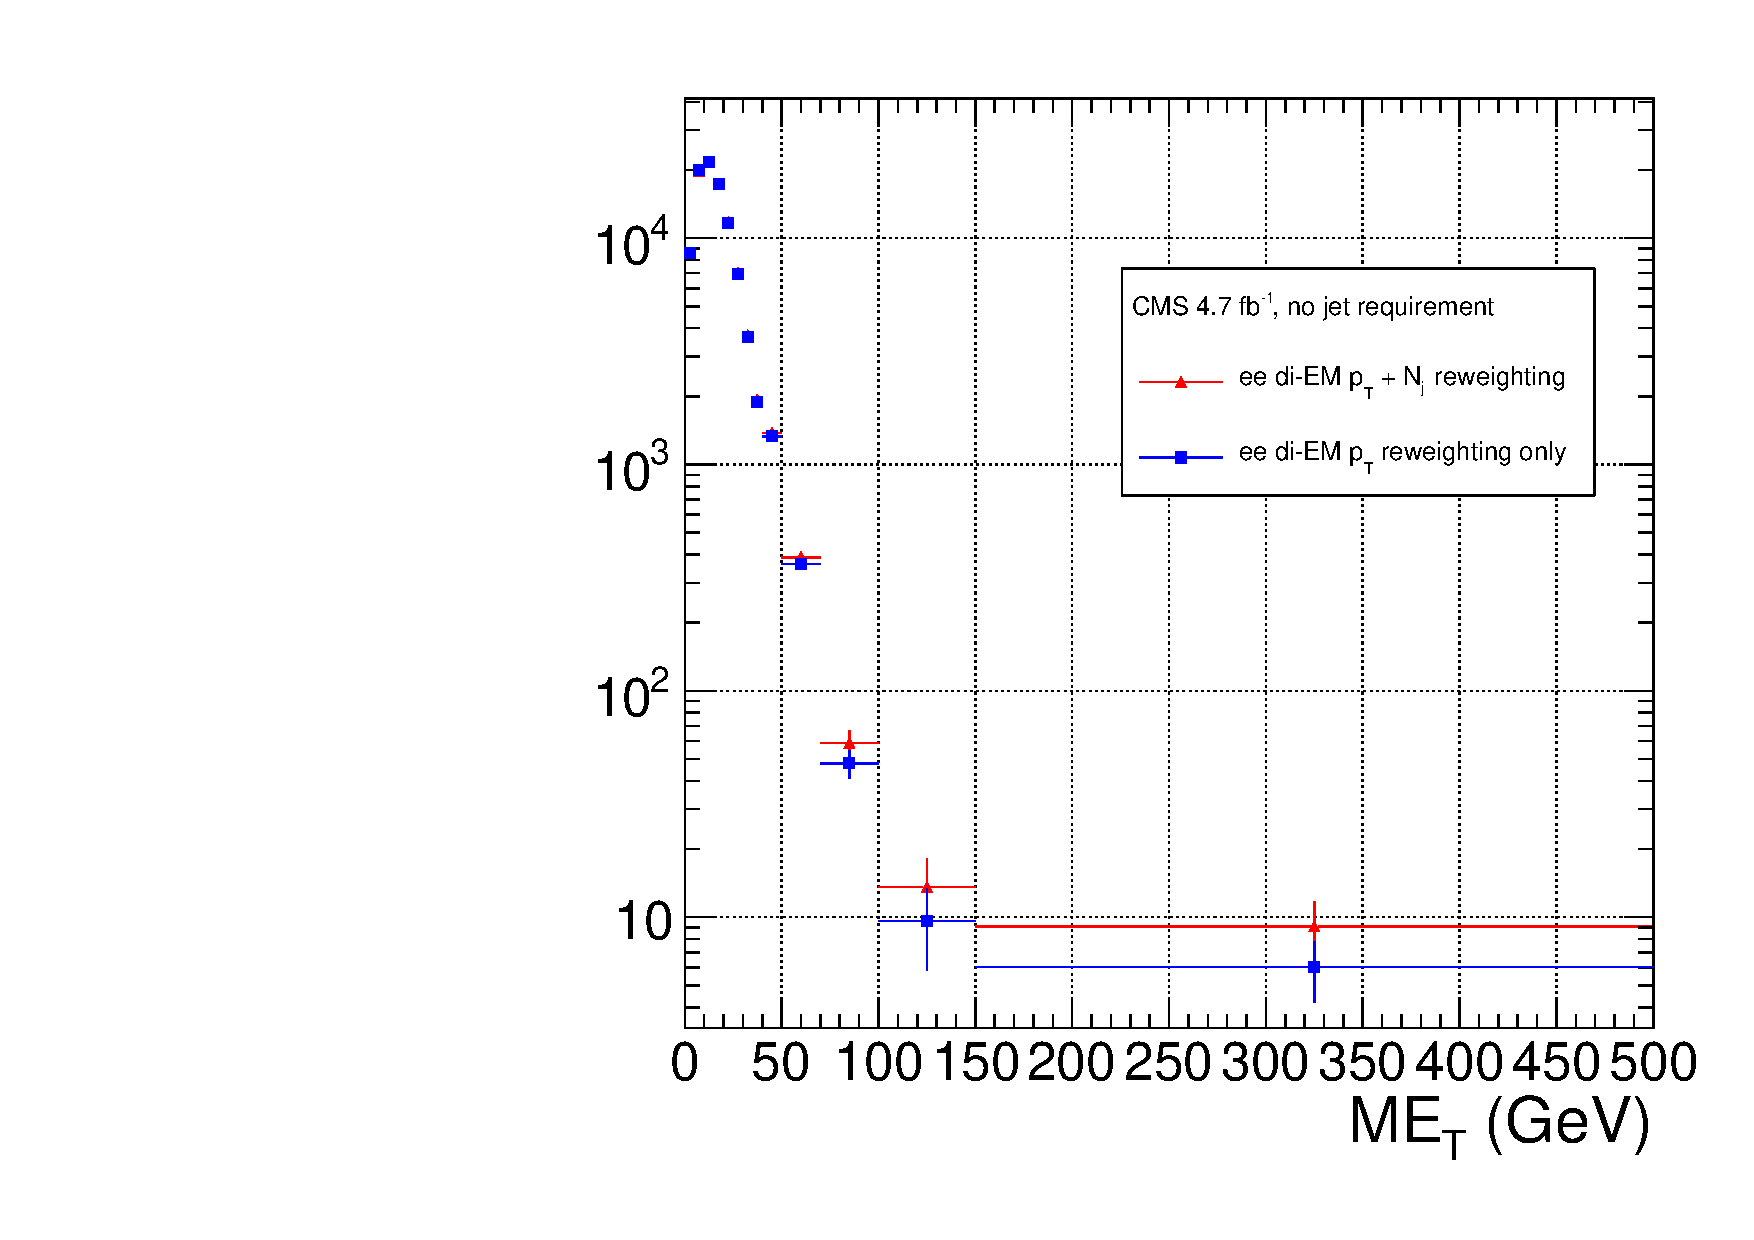
\includegraphics[scale=0.3]{ee_dijet_pT_and_Nj_vs_dijet_pT_reweighting}}
	\hspace{1cm}
	\subfloat[$\mathit{ff}$ \MET spectra.]{\label{fig:ff_dijet_pT_and_Nj_vs_dijet_pT_reweighting}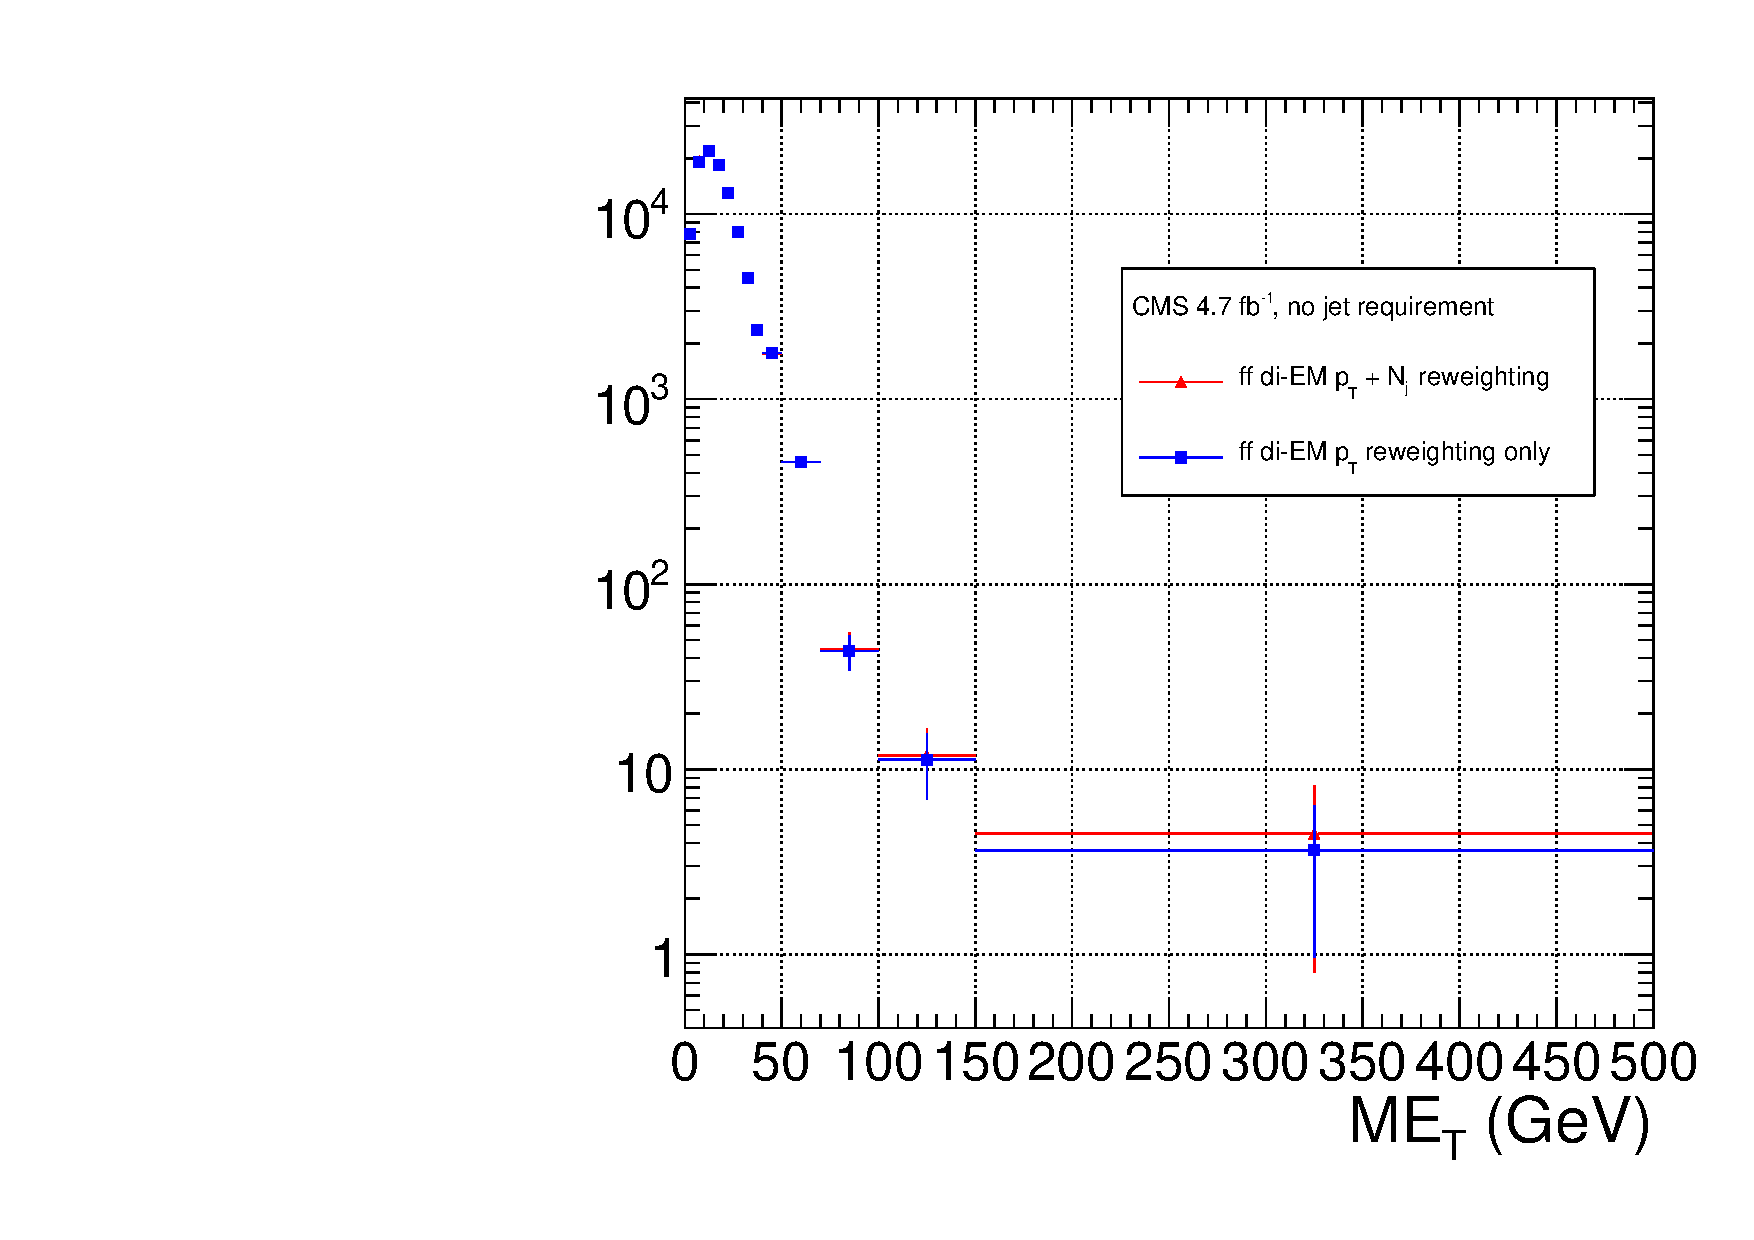
\includegraphics[scale=0.3]{ff_dijet_pT_and_Nj_vs_dijet_pT_reweighting}}
	\\
	\subfloat[Ratio of $ee$ to $\mathit{ff}$ \MET spectra.]{\label{fig:ee_over_ff_dijet_pT_and_Nj_vs_dijet_pT_reweighting}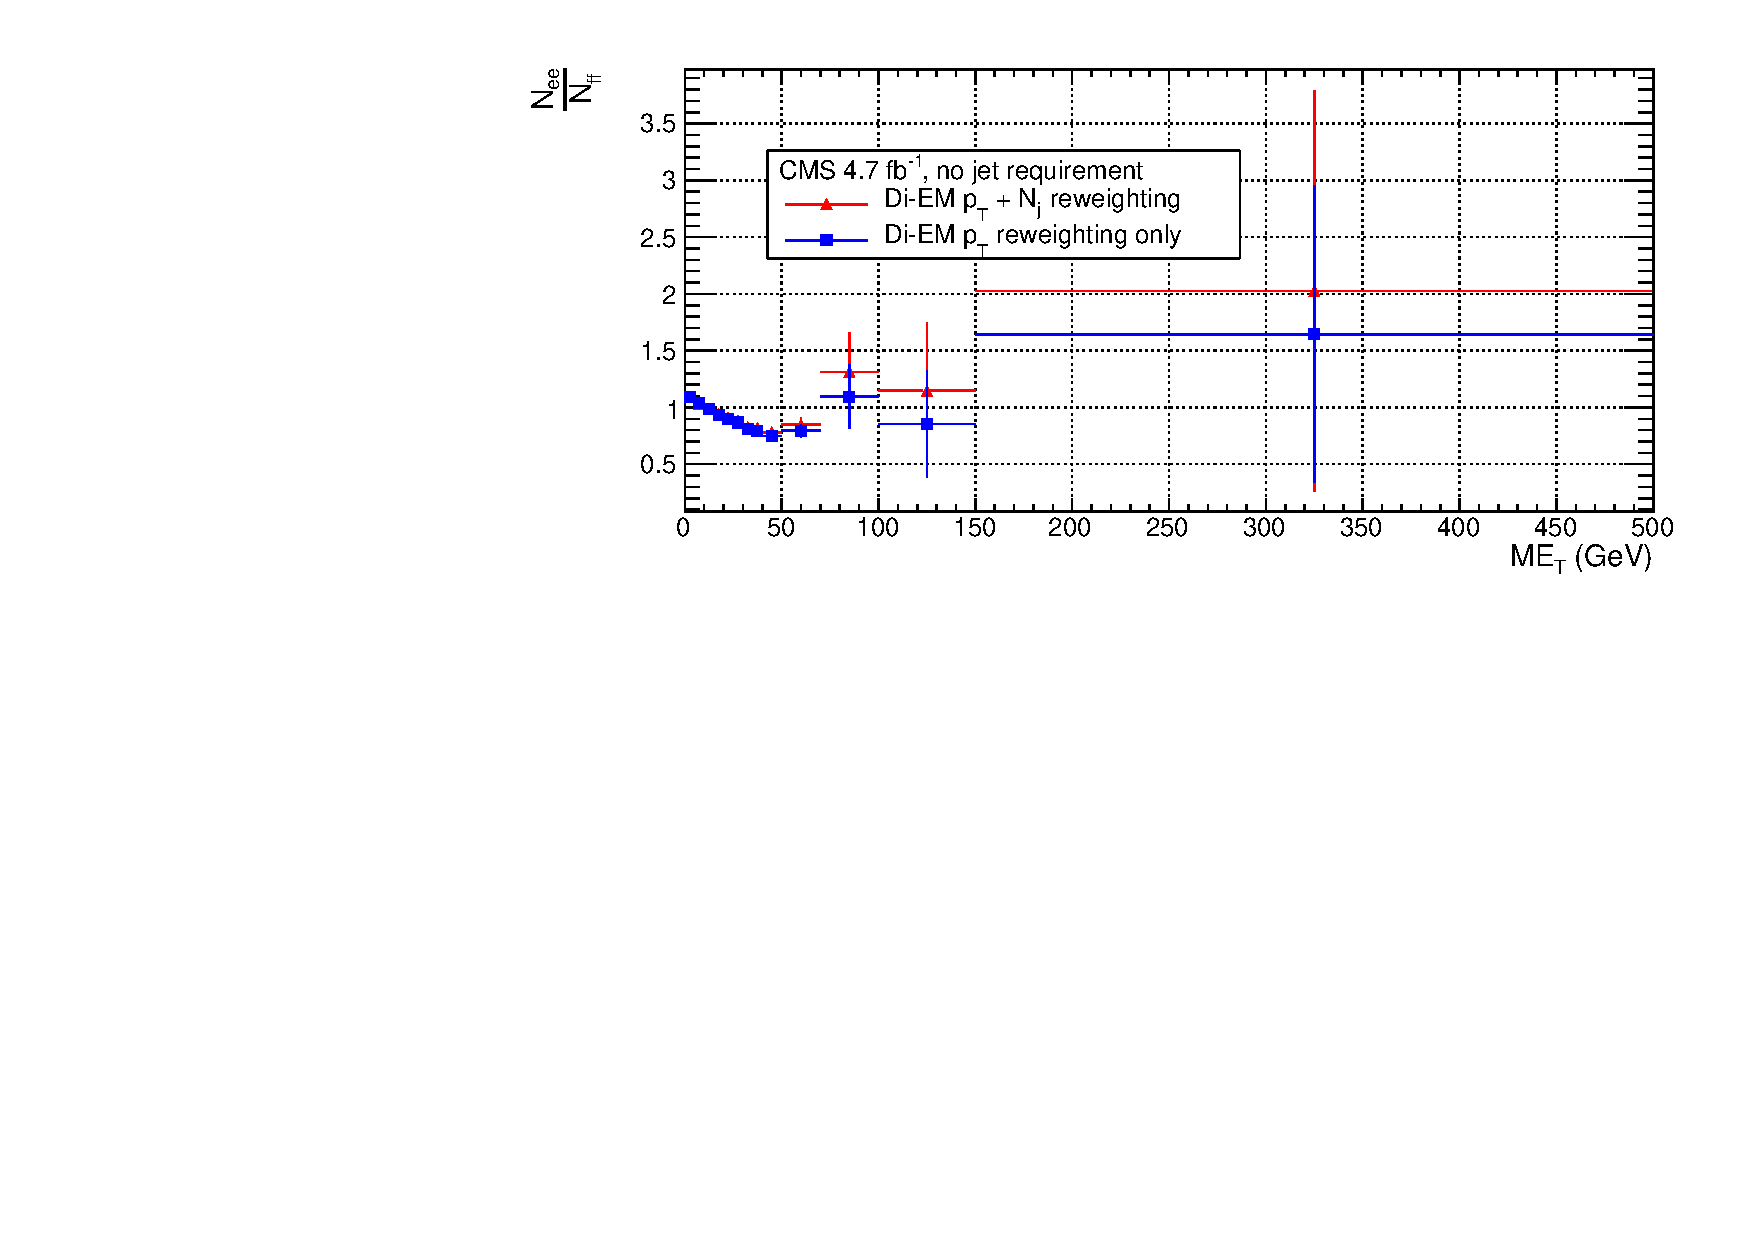
\includegraphics[scale=0.3]{ee_over_ff_dijet_pT_and_Nj_vs_dijet_pT_reweighting}}
	\hspace{1cm}
	\subfloat[Ratio of $ee$ to $\mathit{ff}$ \MET spectra, zoomed x-axis.]{\label{fig:ee_over_ff_dijet_pT_and_Nj_vs_dijet_pT_reweighting_zoom}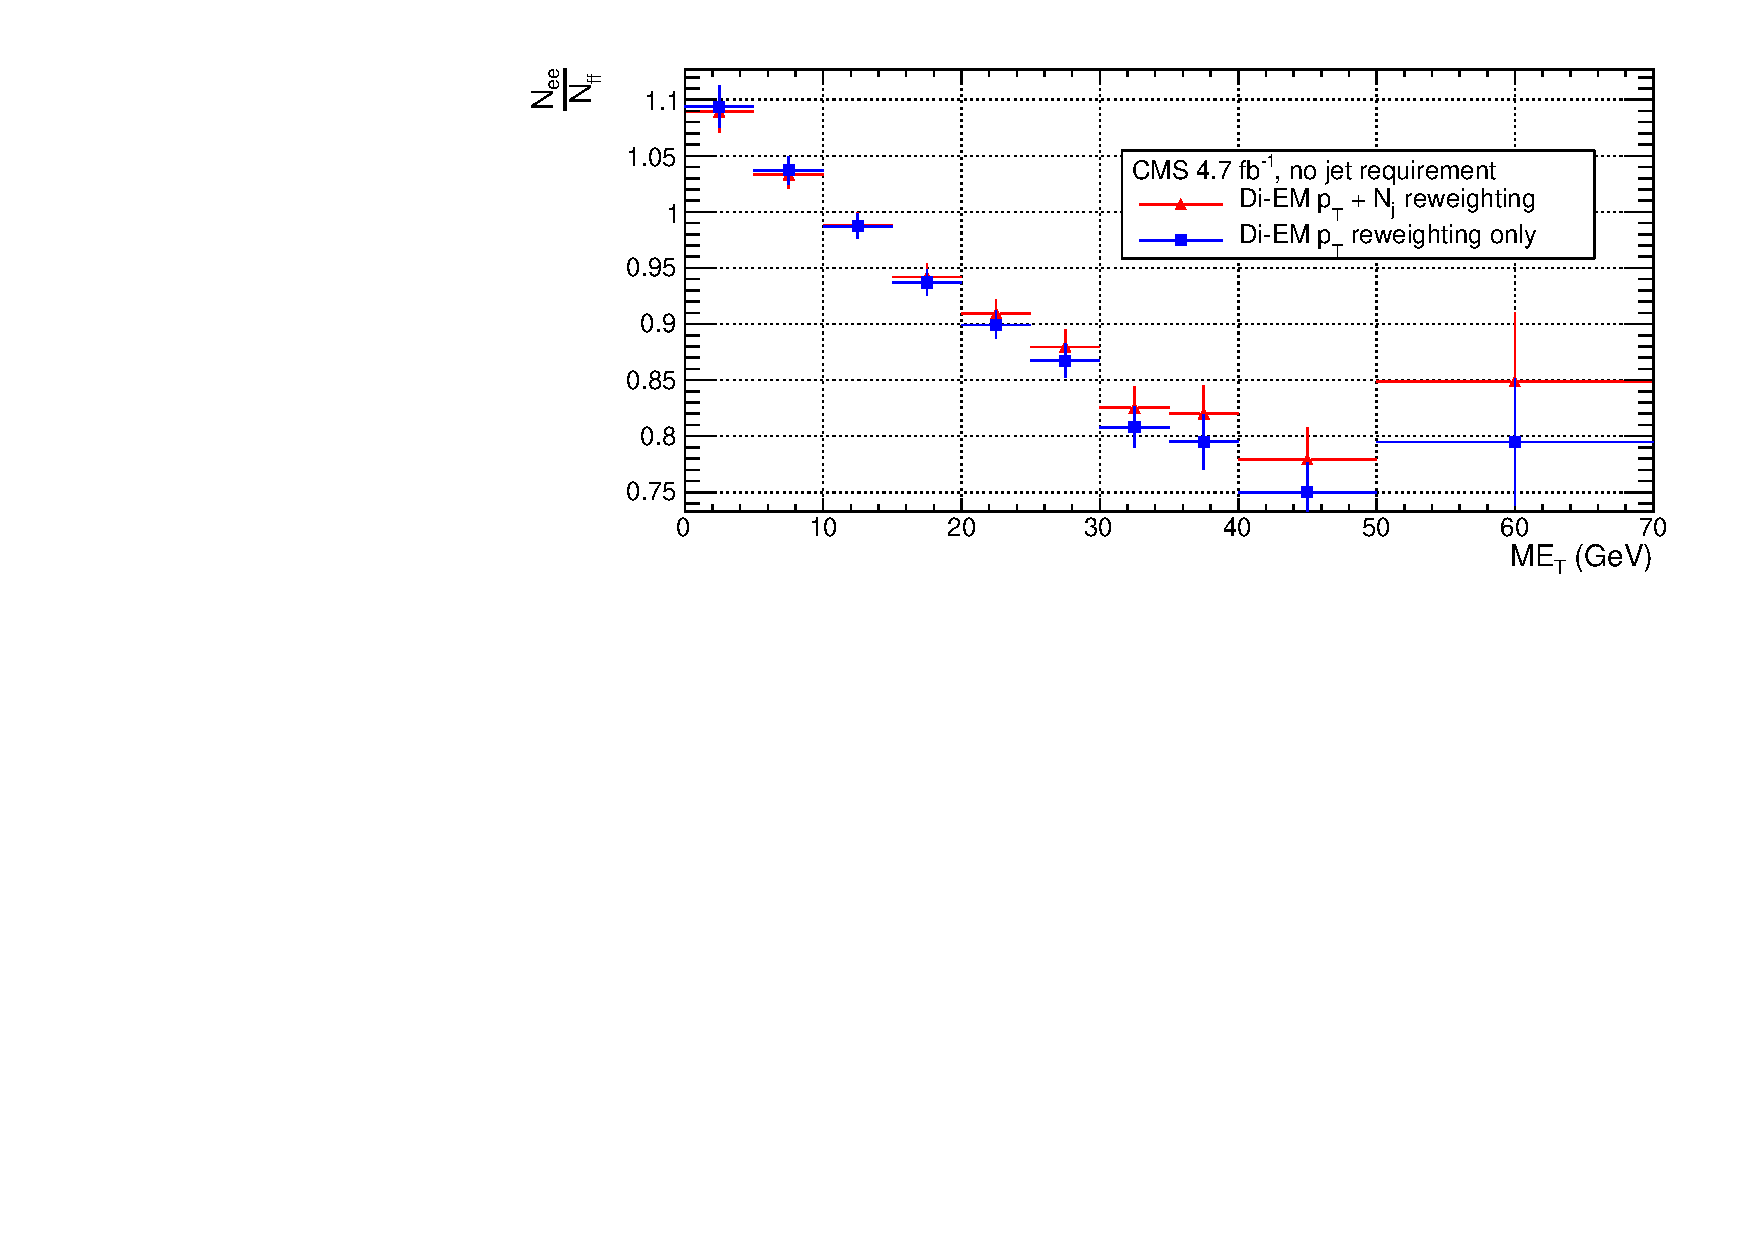
\includegraphics[scale=0.3]{ee_over_ff_dijet_pT_and_Nj_vs_dijet_pT_reweighting_zoom}}
	\caption{\MET spectra of the reweighted $ee$ (81 GeV $\leq m_{\mathrm{ee}} <$ 101 GeV) and $\mathit{ff}$ control samples.  Blue squares indicate di-EM $p_{T}$ reweighting only; red triangles indicate di-EM $p_{T}$ + number of jets reweighting.  PF $p_{T}$ (cf. p.~\pageref{fig:MET_vs_di-EM_pT}) is used to calculate the di-EM $p_{T}$.  The full normalization procedure is employed, along with $ee$ sideband subtraction (discussed at the end of this section).  Error bars are statistical only.}
	\label{fig:dijet_pT_and_Nj_vs_dijet_pT_reweighting}
\end{figure}

Although the electron and photon energies are well measured by the ECAL, the ECAL-only measurement of the fake photon energy (cf. Sec~\ref{sec:Photons}) is biased slightly low due to the fact that fakes (which are really jets) tend to deposit some energy in the HCAL.  This can be seen in Figs.~\ref{fig:ET_bias_vs_EMF} and~\ref{fig:4684pb-1_single_ETBias}, which show the relative difference between the ECAL-only $E_{T}$ measurement and the PF $E_{T}$ measurement vs. EMF for electrons, photons, and fakes.  PF $E_{T}$ is defined as the \verb+L1Fast+-corrected $E_{T}$ of the nearest PF jet with $p_{T} \geq 20$ GeV (i.e., the $E_{T}$ of the PF jet object reconstructed from the same ECAL shower as the fake photon).  On average, the fakes tend to deposit a few percent more energy in the HCAL than the electrons or photons, which is recovered by the PF algorithm.  For this reason, the PF $p_{T}$ is used in the calculation of di-EM $p_{T}$ rather than the ECAL-only $p_{T}$.\footnote{In the few events ($\mathcal{O}(10^{-3})$) in which two PF jet objects, corresponding to the two electrons or fakes, are not found, the ECAL-only $p_{T}$ is used.}  This leads to a modest improvement in the agreement between the $ee$ and $\mathit{ff}$ \MET spectra, as shown in Figure~\ref{fig:ee_vs_ff_di-EM_vs_dijet_pT_reweighting}.

%include similar figures for MC?
\begin{figure}
	\centering
	\subfloat[Leading electron in $ee$ events.]{\label{fig:4684pb-1_eLeading_ETBias_log}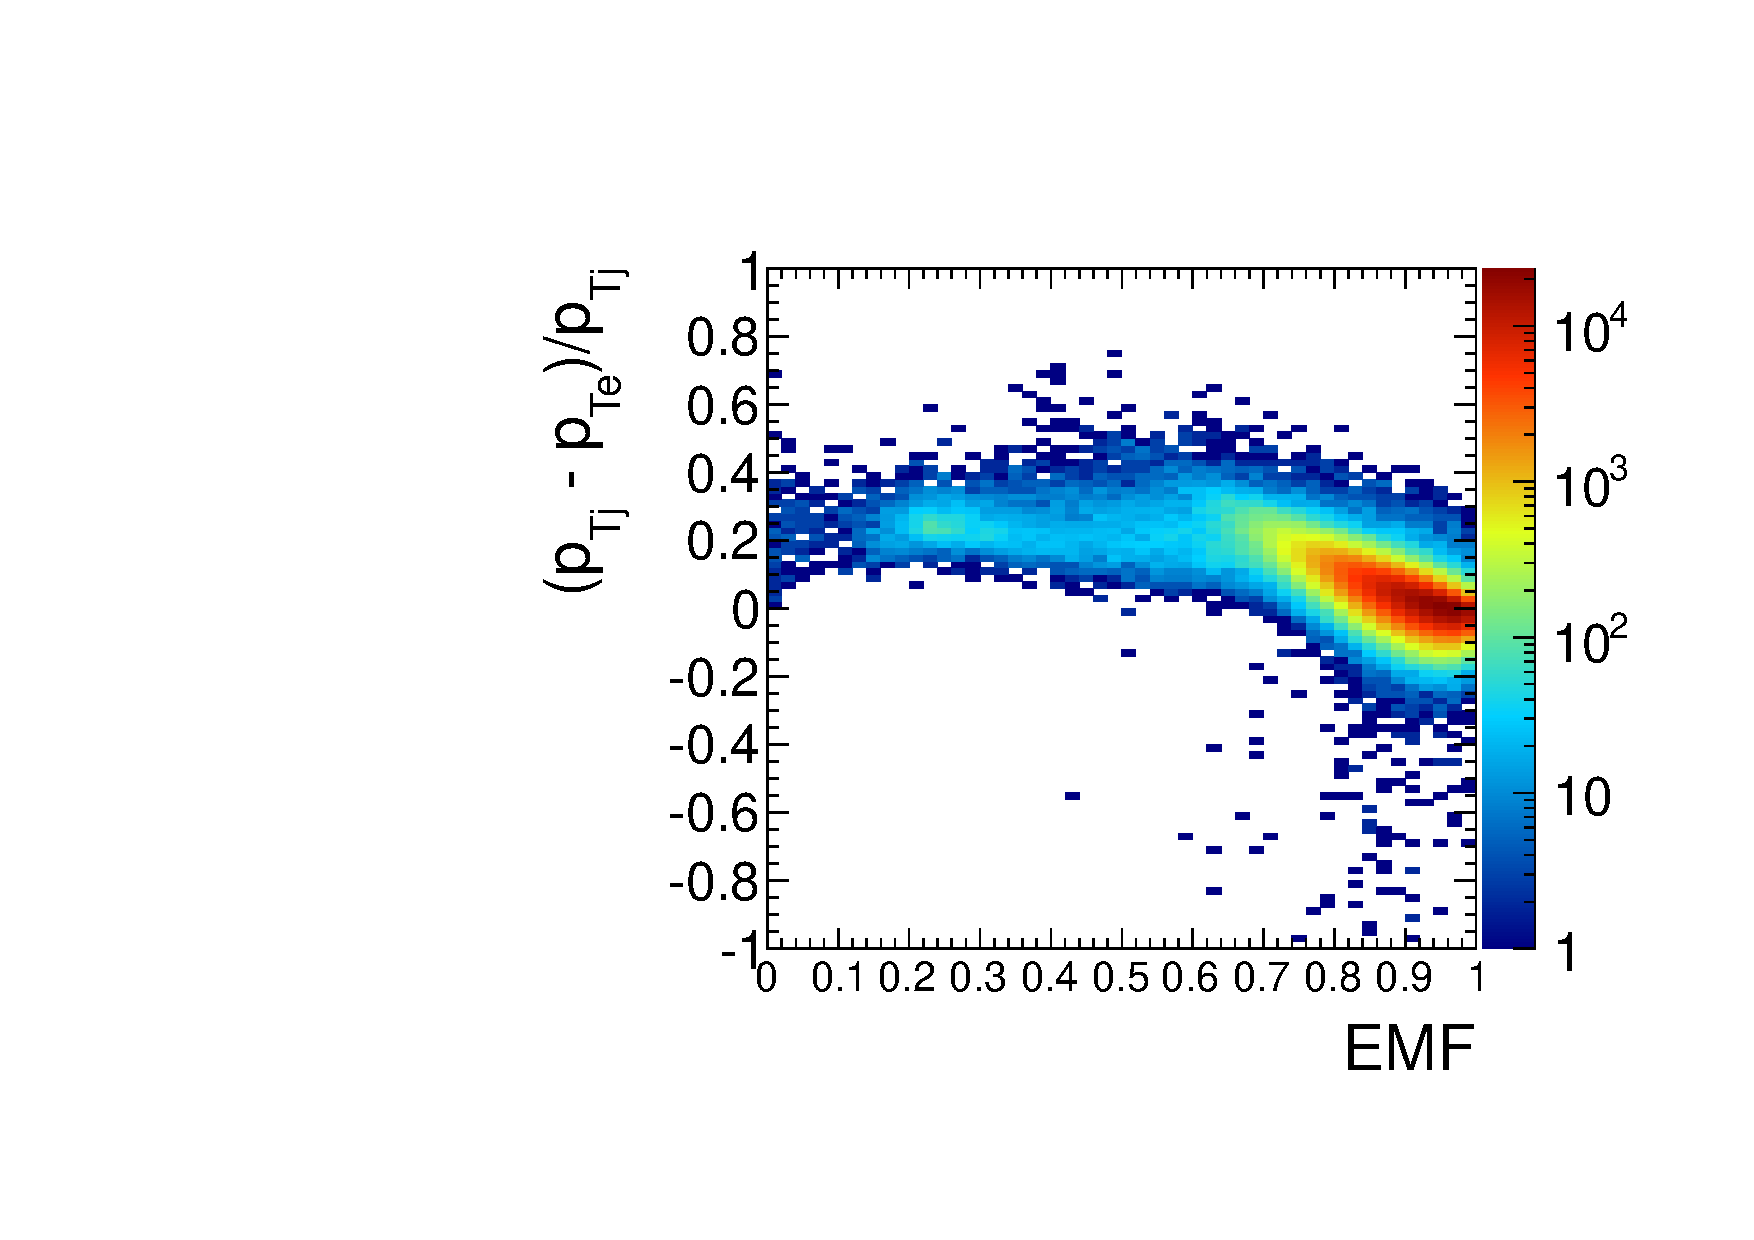
\includegraphics[scale=0.25]{4684pb-1_eLeading_ETBias_log}}
	\hspace{1cm}
	\subfloat[Trailing electron in $ee$ events.]{\label{fig:4684pb-1_eTrailing_ETBias_log}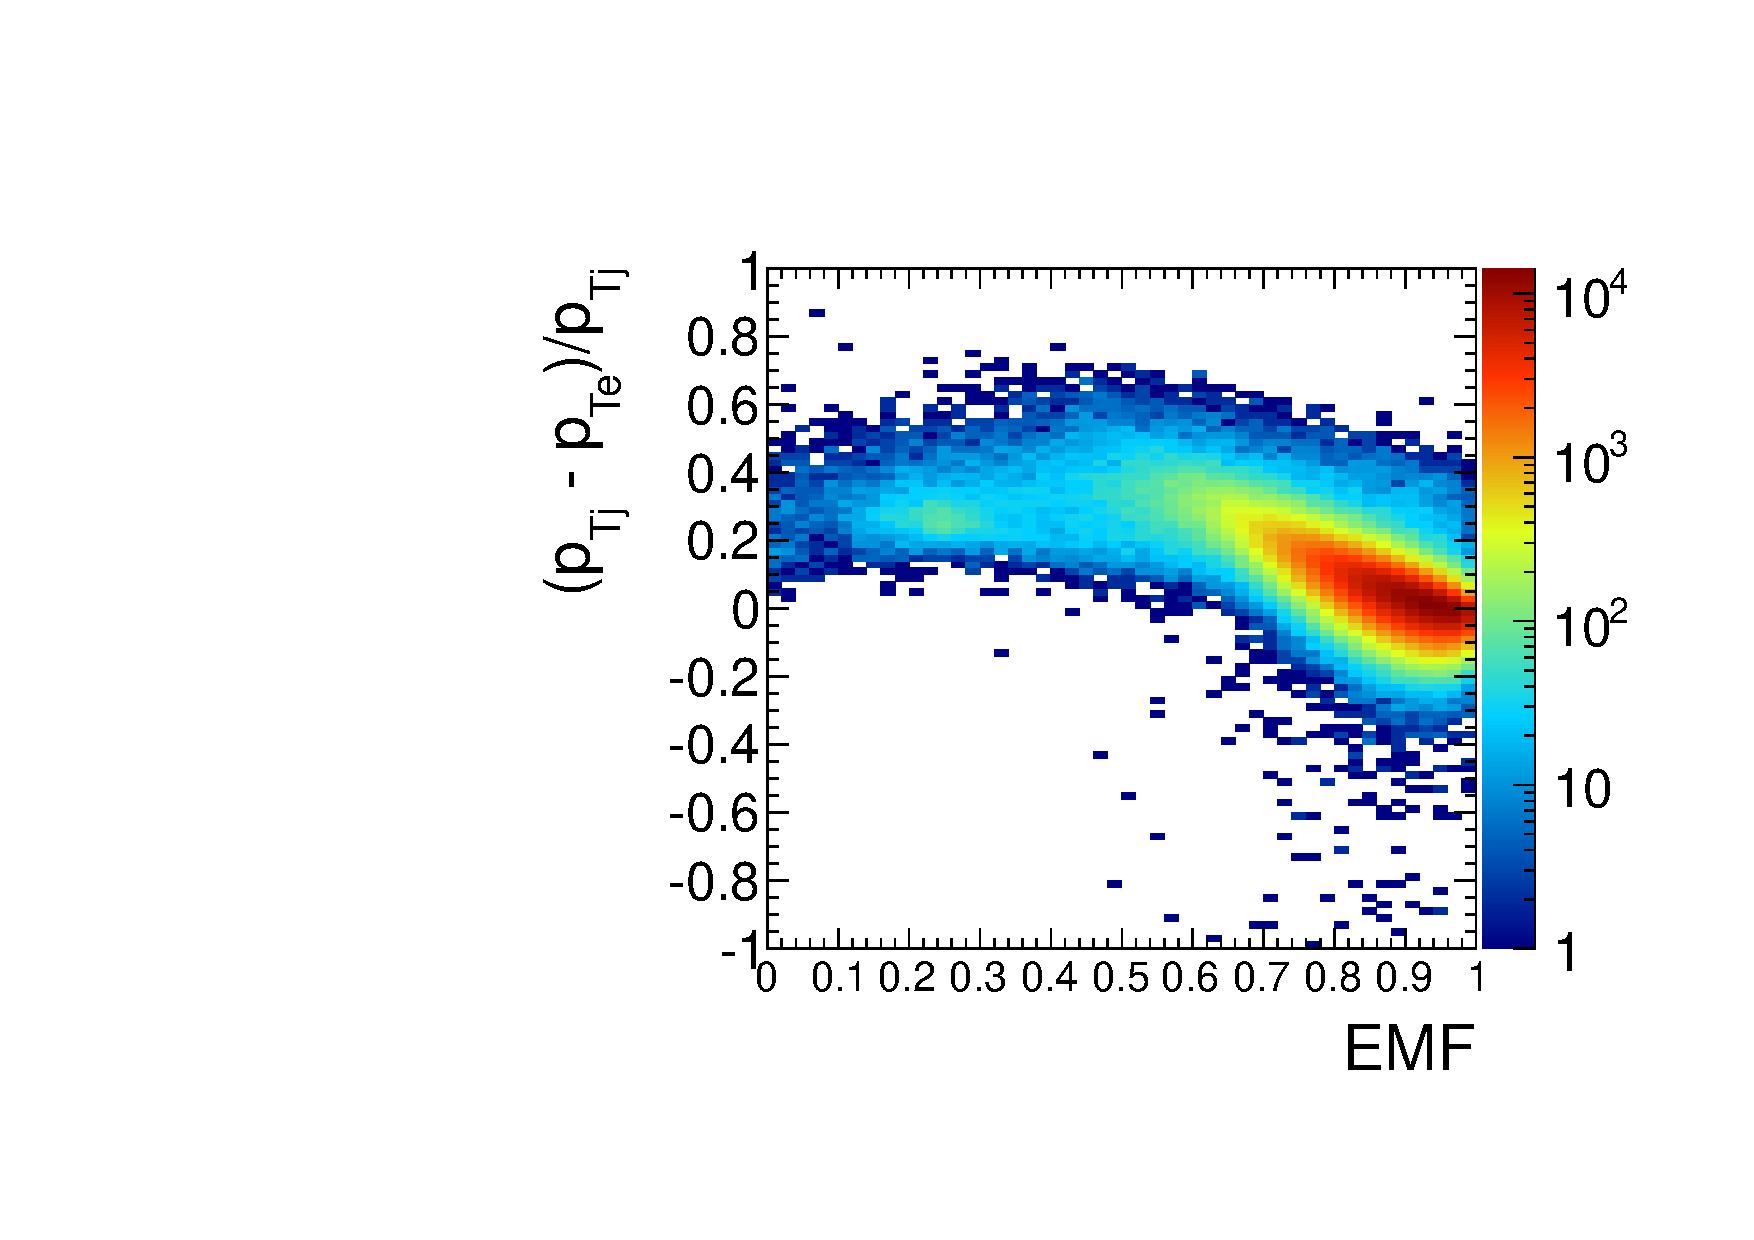
\includegraphics[scale=0.25]{4684pb-1_eTrailing_ETBias_log}}
	\\
	\subfloat[Leading fake in $\mathit{ff}$ events.]{\label{fig:4684pb-1_fLeading_ETBias_log}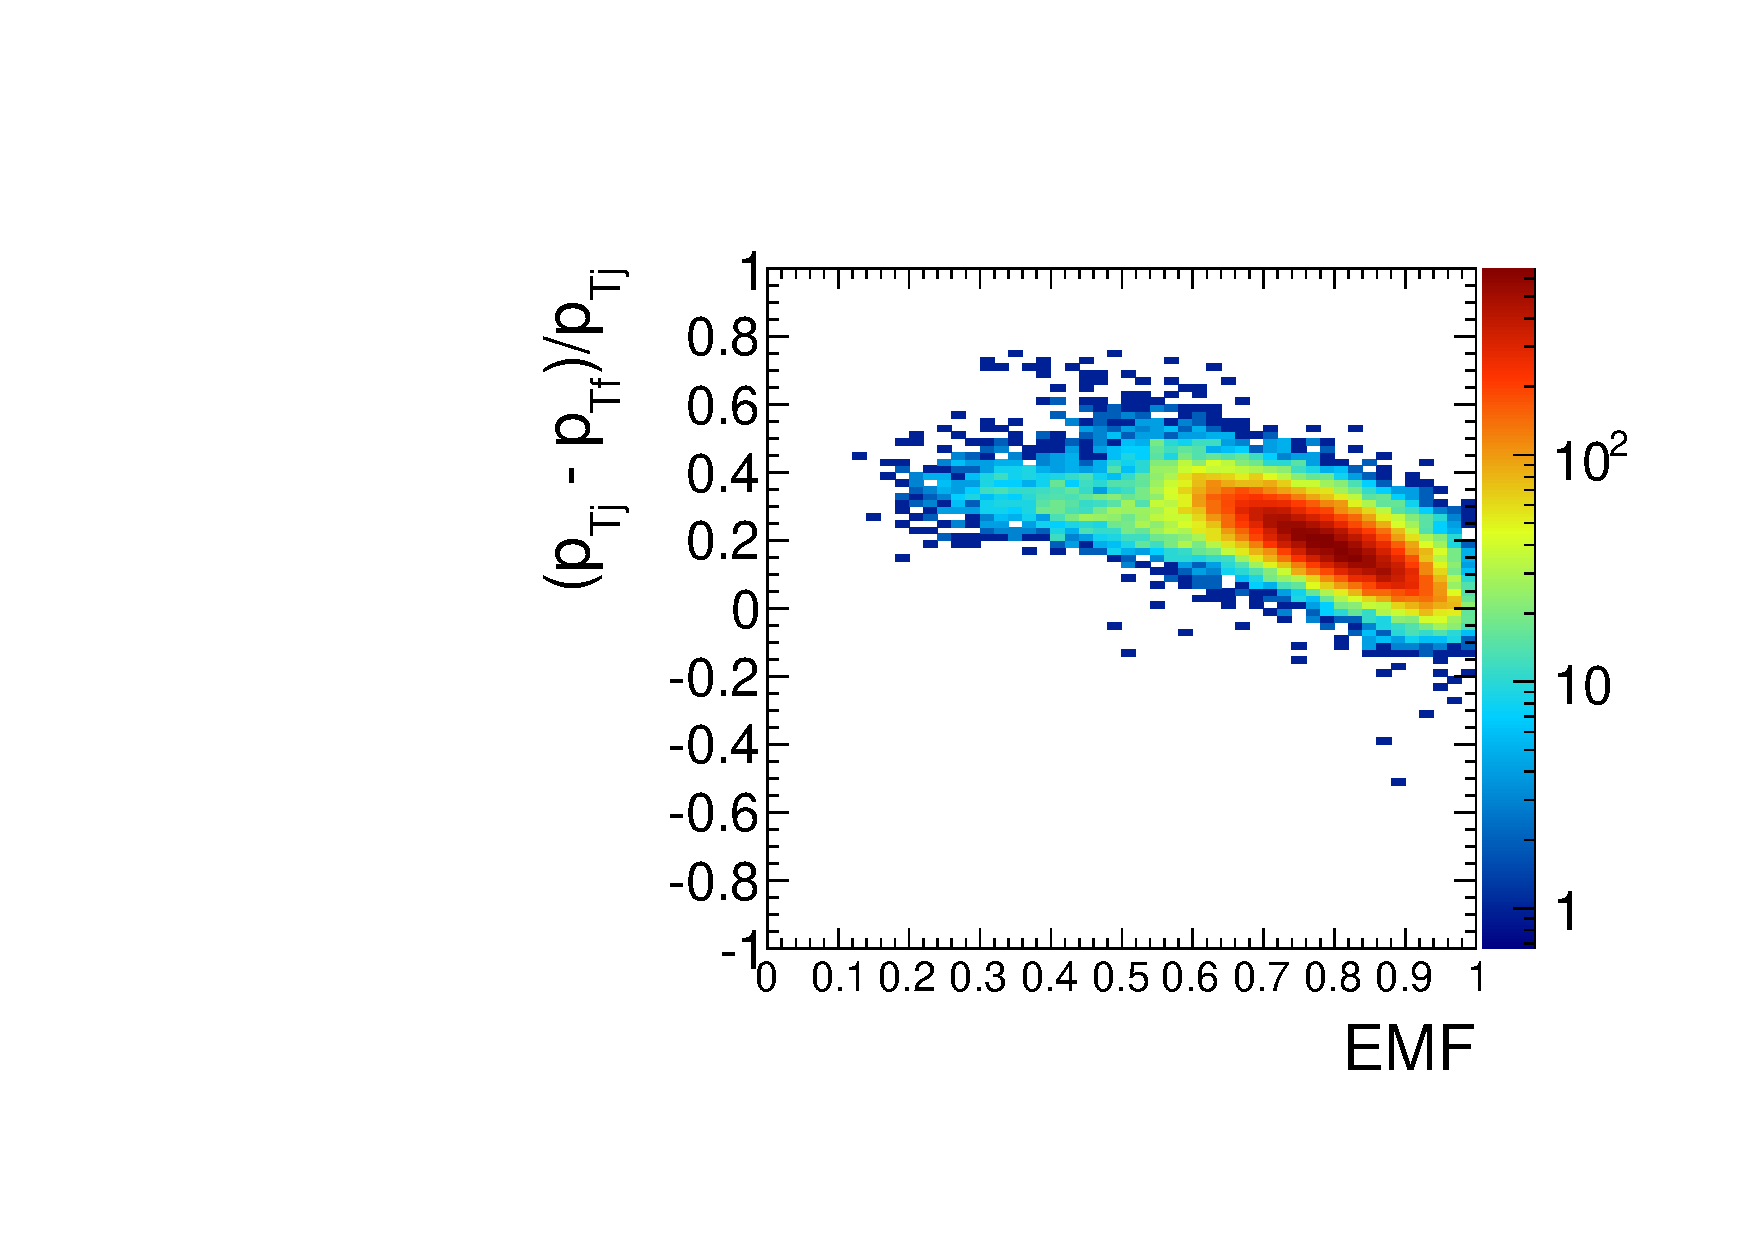
\includegraphics[scale=0.25]{4684pb-1_fLeading_ETBias_log}}
	\hspace{1cm}
	\subfloat[Trailing fake in $\mathit{ff}$ events.]{\label{fig:4684pb-1_fTrailing_ETBias_log}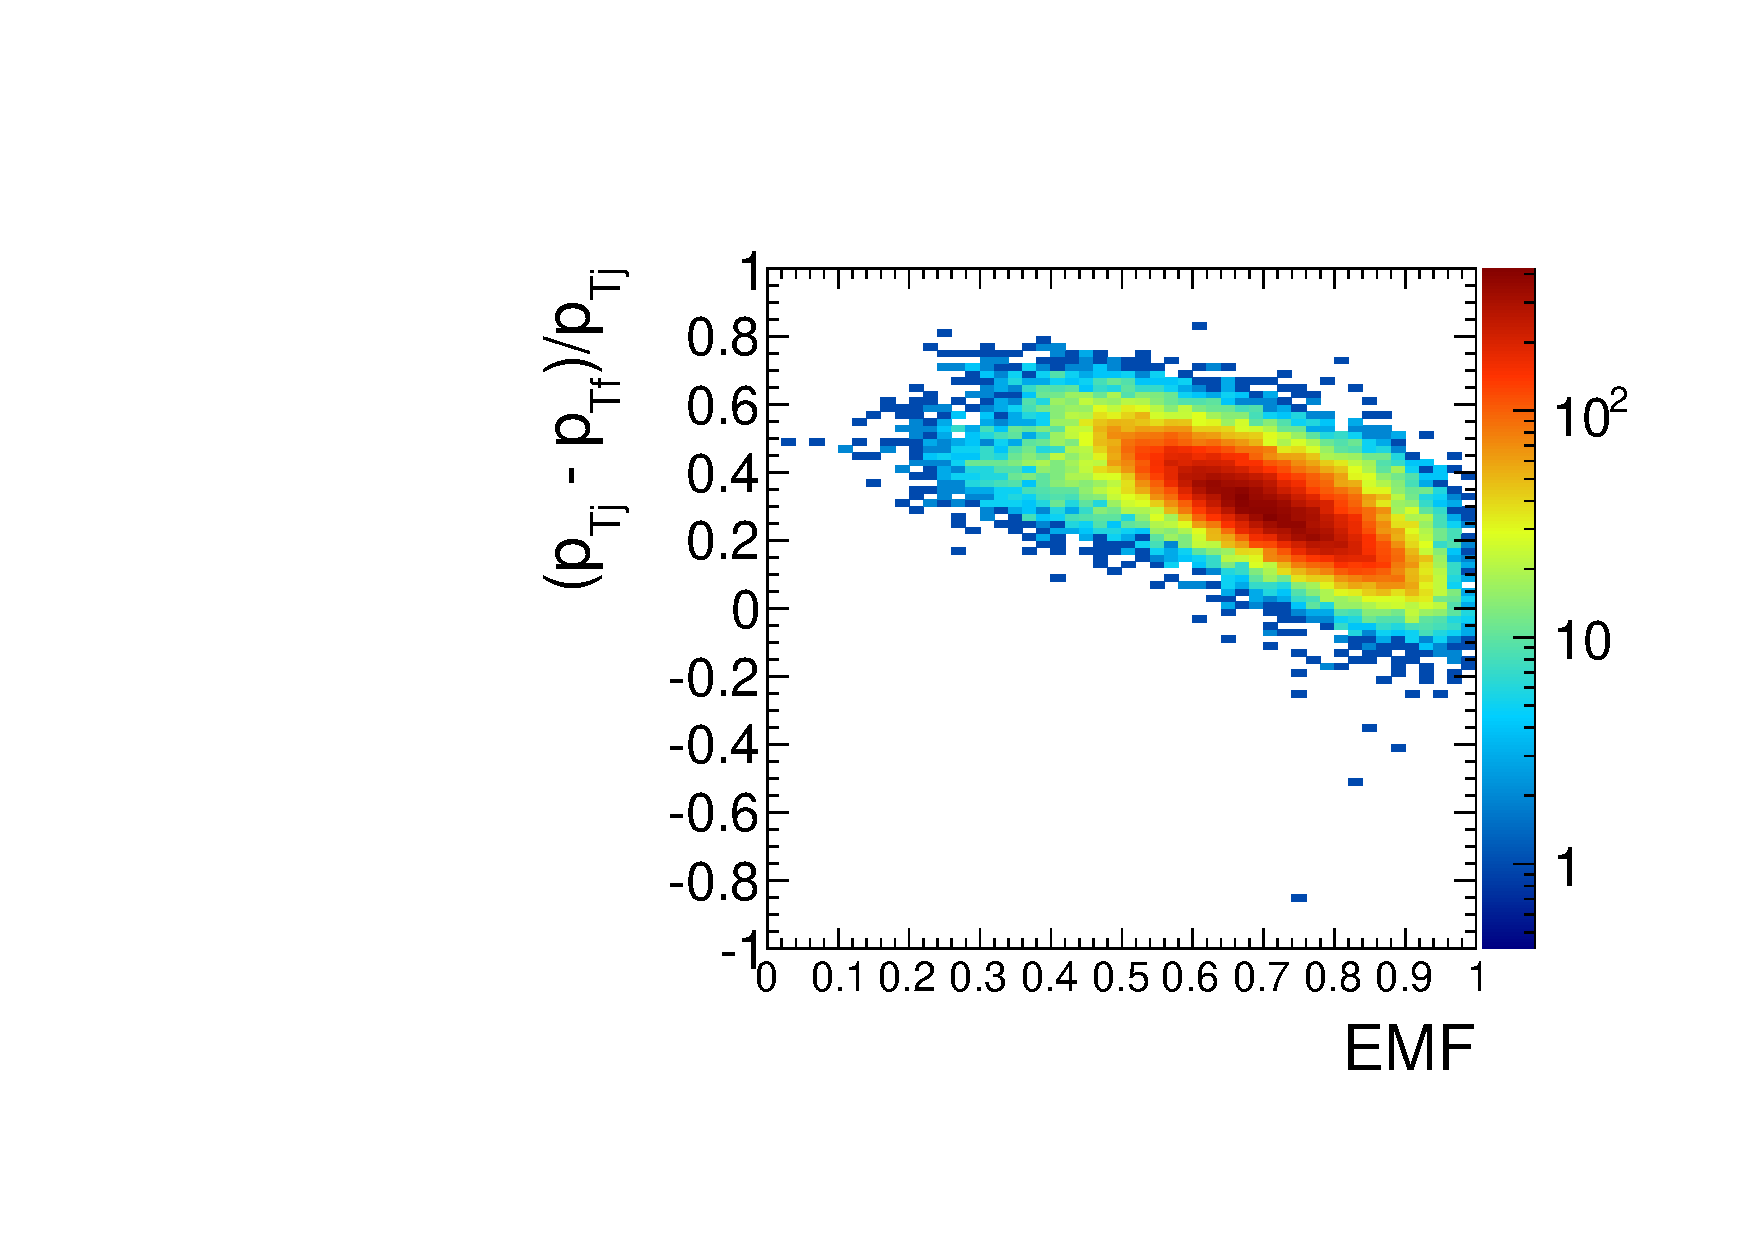
\includegraphics[scale=0.25]{4684pb-1_fTrailing_ETBias_log}}
	\\
	\subfloat[Leading photon in $\gamma\gamma$ events.]{\label{fig:4684pb-1_gLeading_ETBias_log}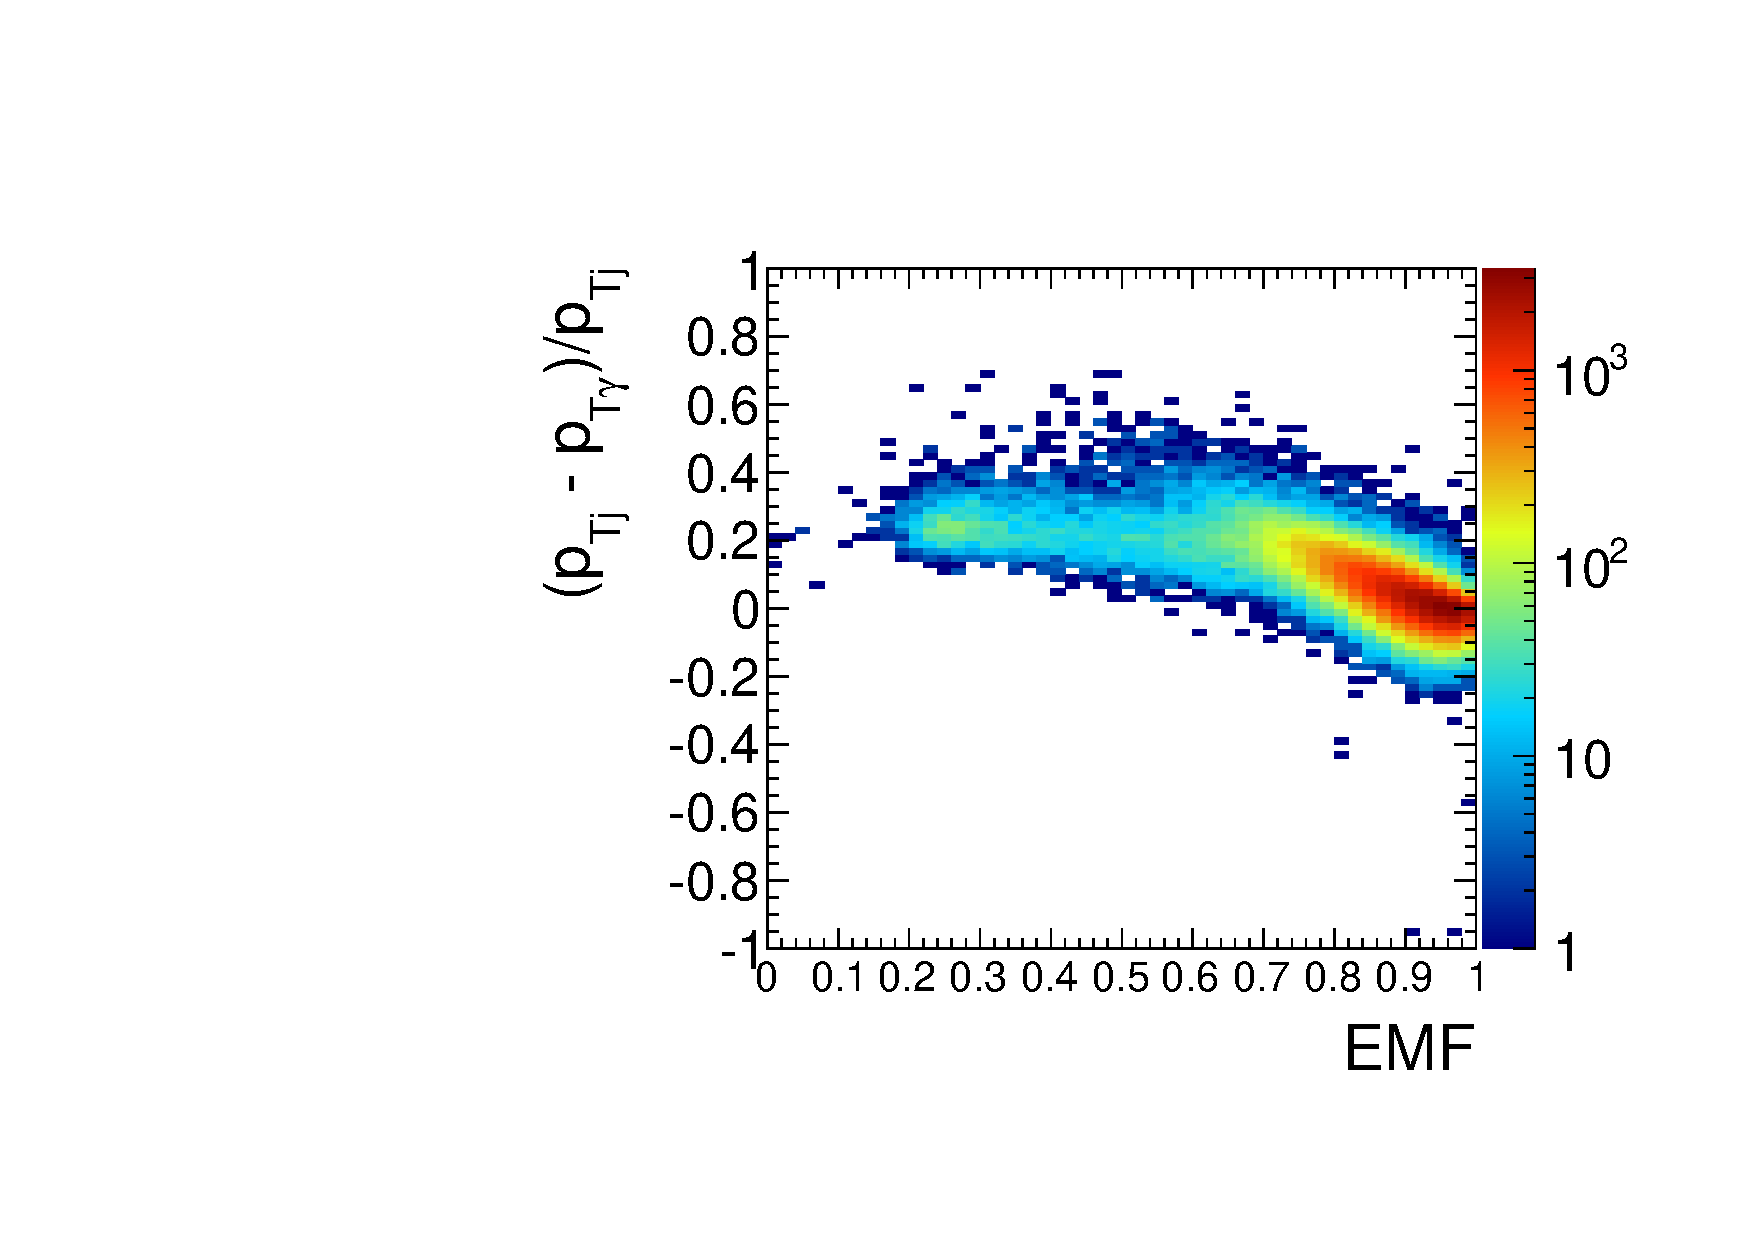
\includegraphics[scale=0.25]{4684pb-1_gLeading_ETBias_log}}
	\hspace{1cm}
	\subfloat[Trailing photon in $\gamma\gamma$ events.]{\label{fig:4684pb-1_gTrailing_ETBias_log}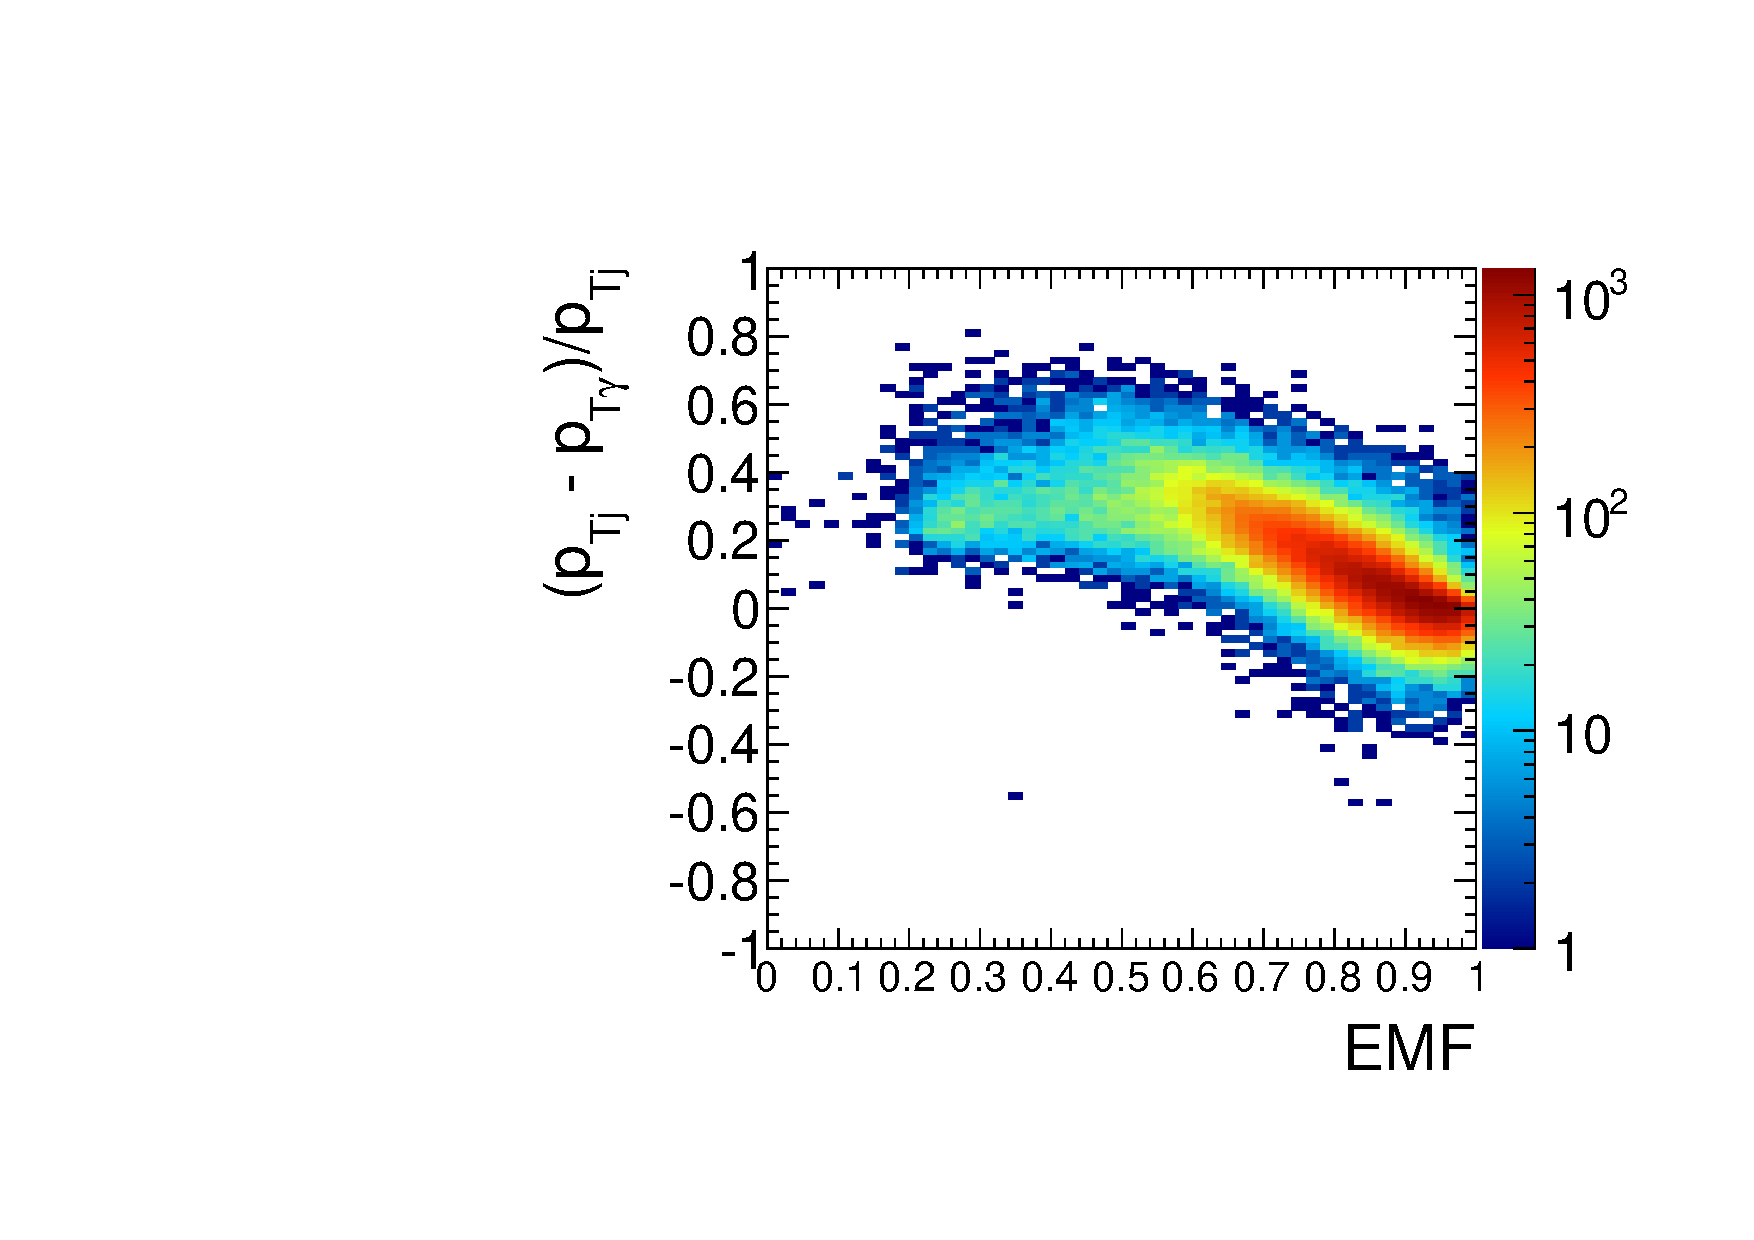
\includegraphics[scale=0.25]{4684pb-1_gTrailing_ETBias_log}}
	\caption{Relative difference between the ECAL-only $E_{T}$ measurement and the PF $E_{T}$ measurement vs. EMF.  PF $E_{T}$ is defined in the text.}
	\label{fig:ET_bias_vs_EMF}
\end{figure}

%include similar figures for MC?
\begin{figure}
	\centering
	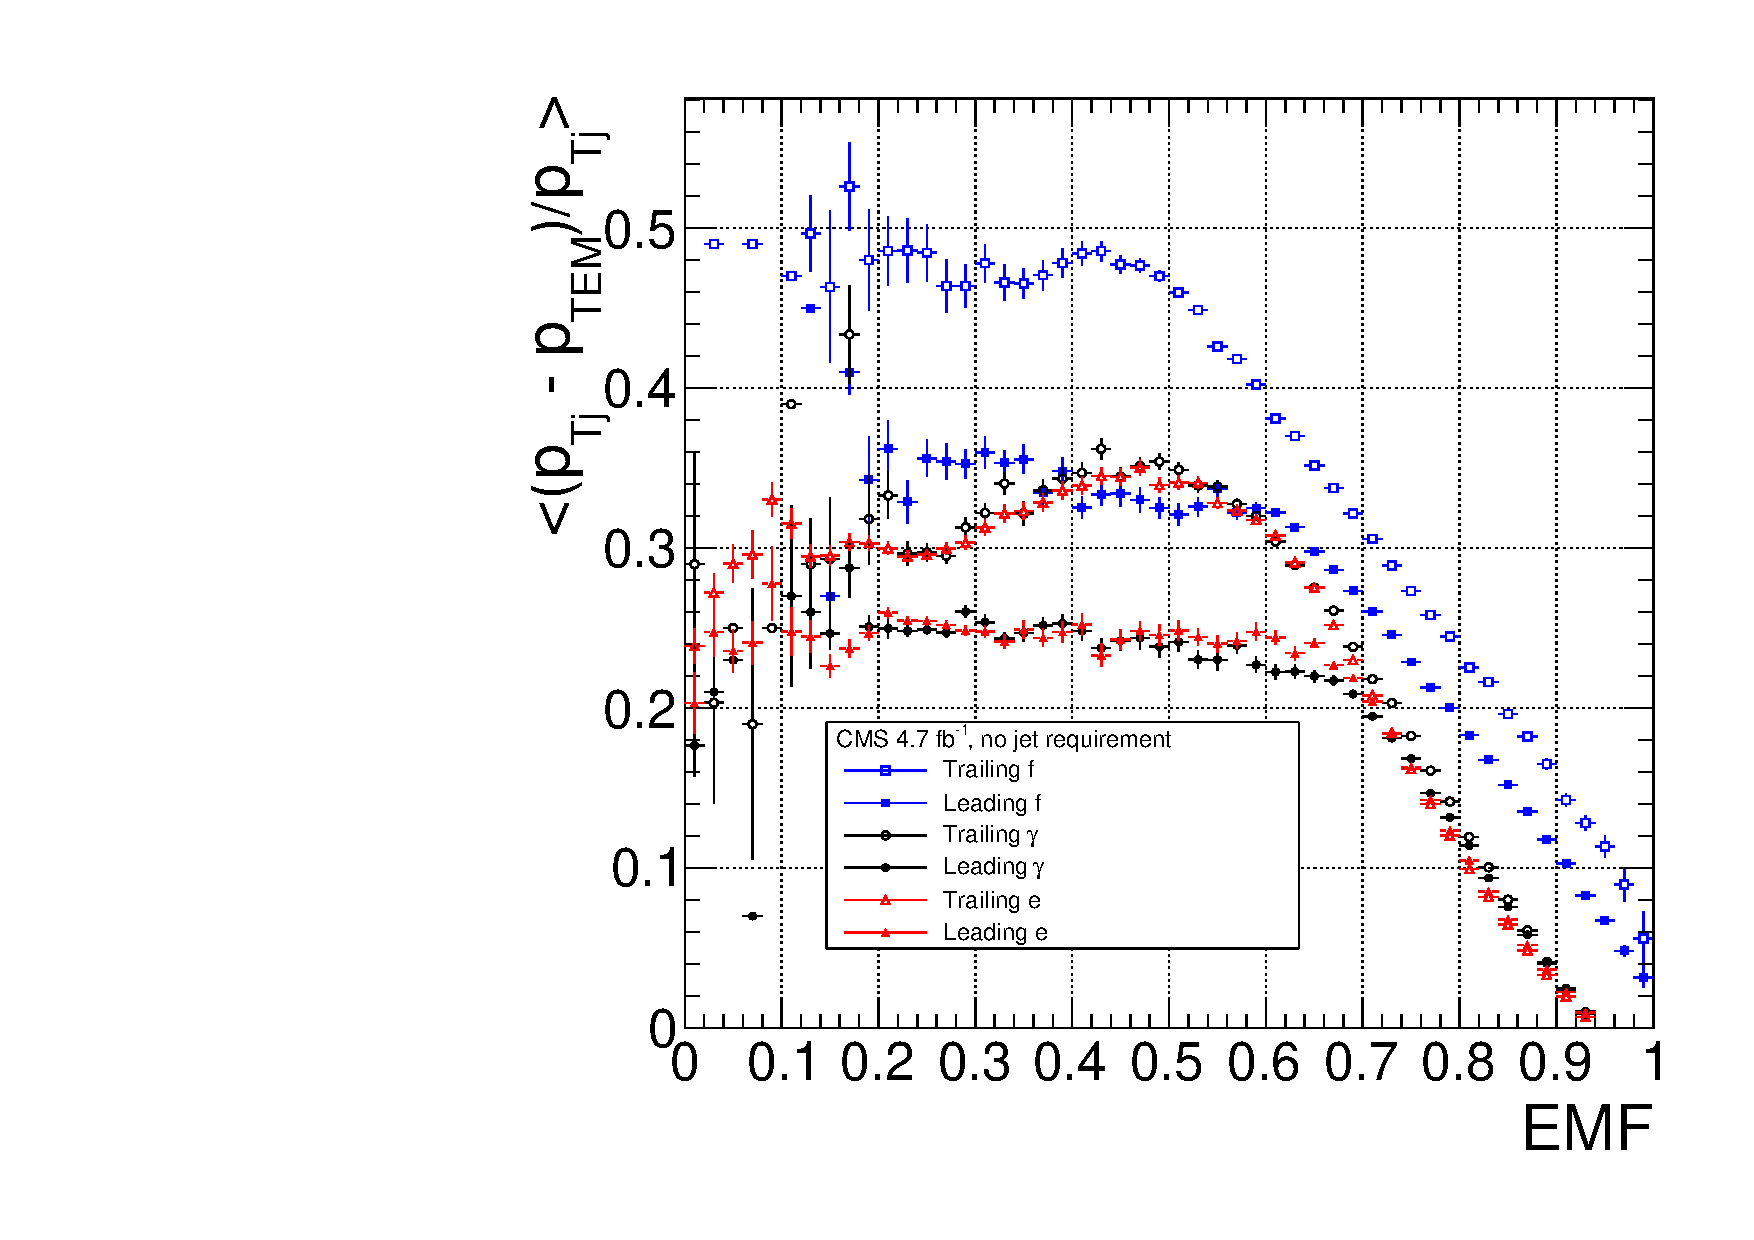
\includegraphics[scale=0.5]{4684pb-1_single_ETBias}
	\caption{Average relative difference between the ECAL-only $E_{T}$ measurement and the PF $E_{T}$ measurement vs. EMF for the leading (filled marker) and trailing (open marker) electrons in $ee$ events (red triangles), fakes in $\mathit{ff}$ events (blue squares), and photons in $\gamma\gamma$ events (black circles).  These are nothing more than profile histograms of Fig.~\ref{fig:ET_bias_vs_EMF}.  PF $E_{T}$ is defined in the text.  Error bars are statistical only.}
	\label{fig:4684pb-1_single_ETBias}
\end{figure}

%include ee/gg and ff/gg agreement?
%include similar figures for MC?
\begin{figure}
	\centering
	\subfloat[$ee$ \MET spectra.]{\label{fig:ee_di-EM_vs_dijet_pT_reweighting}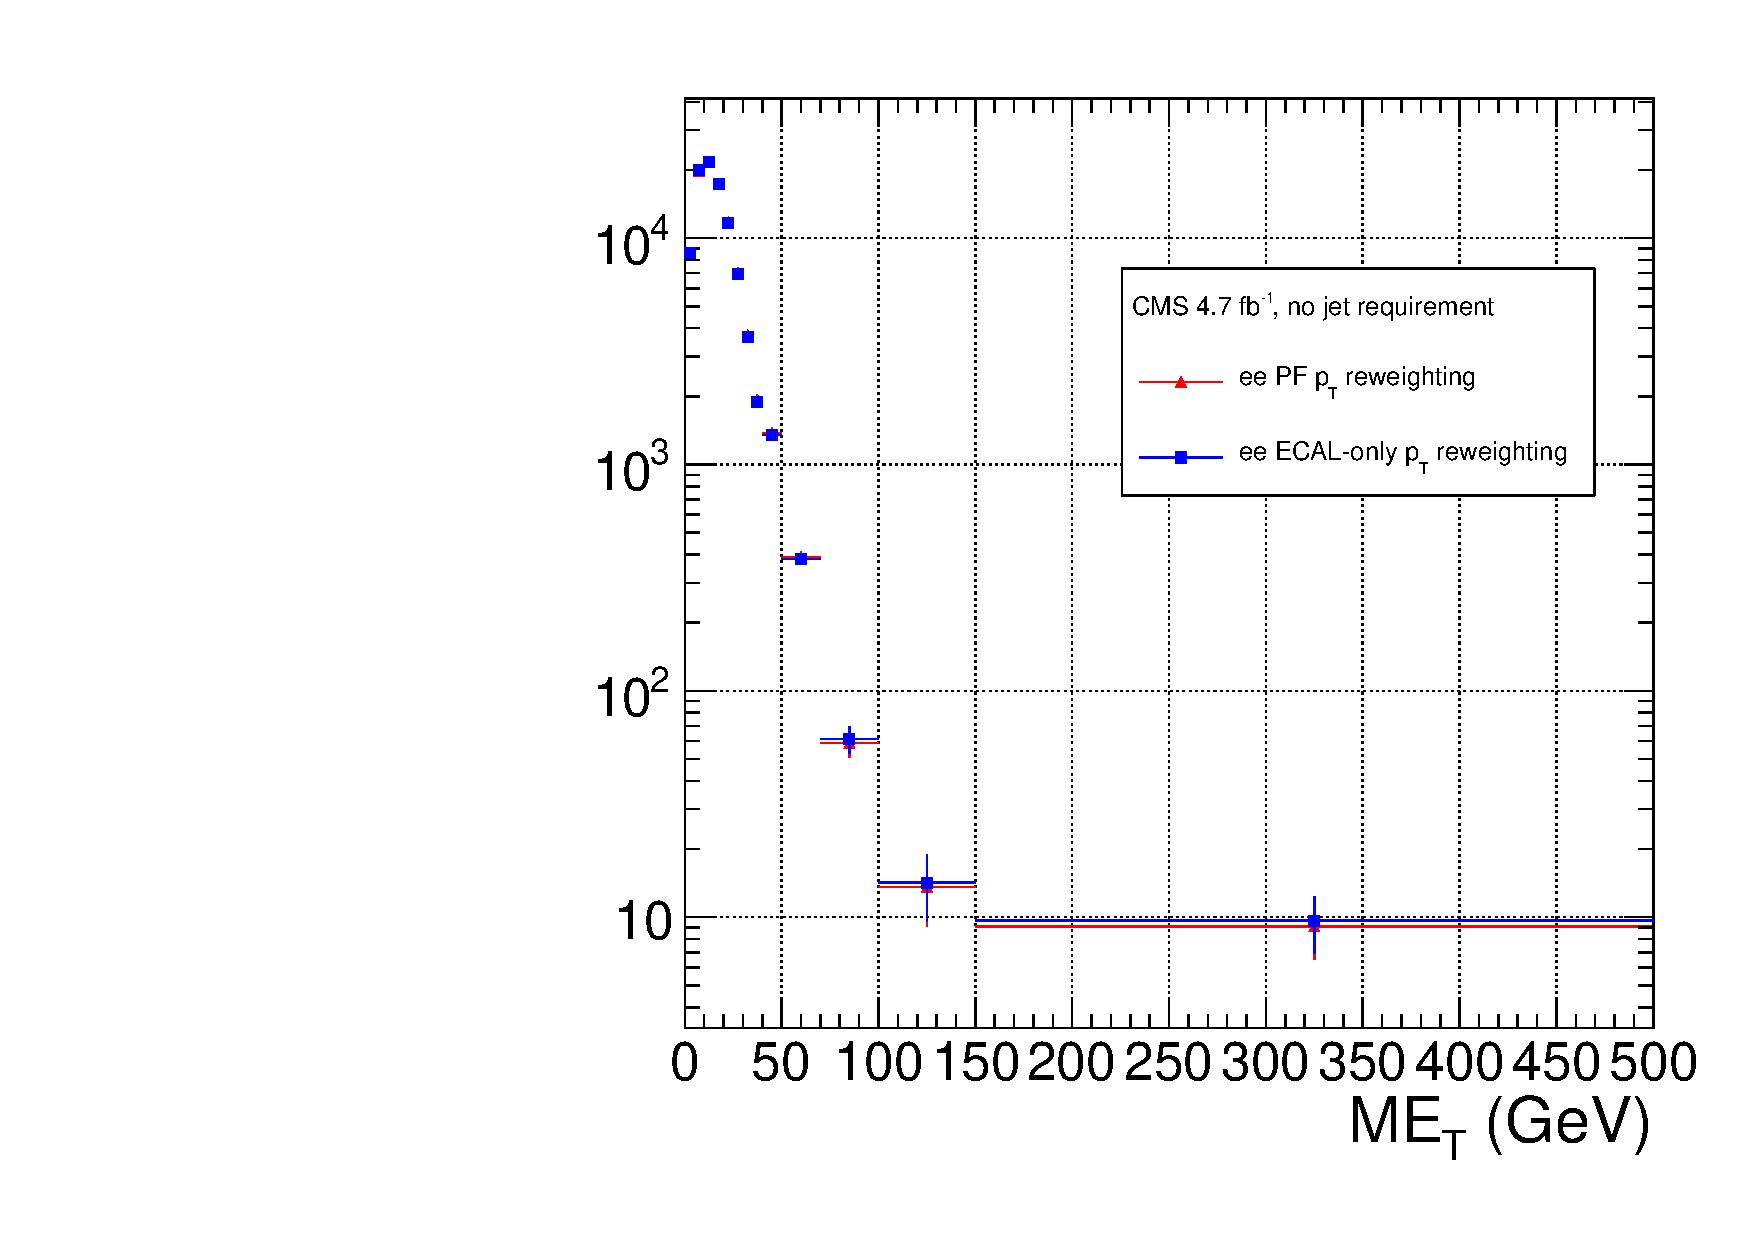
\includegraphics[scale=0.3]{ee_di-EM_vs_dijet_pT_reweighting}}
	\hspace{1cm}
	\subfloat[$\mathit{ff}$ \MET spectra.]{\label{fig:ff_di-EM_vs_dijet_pT_reweighting}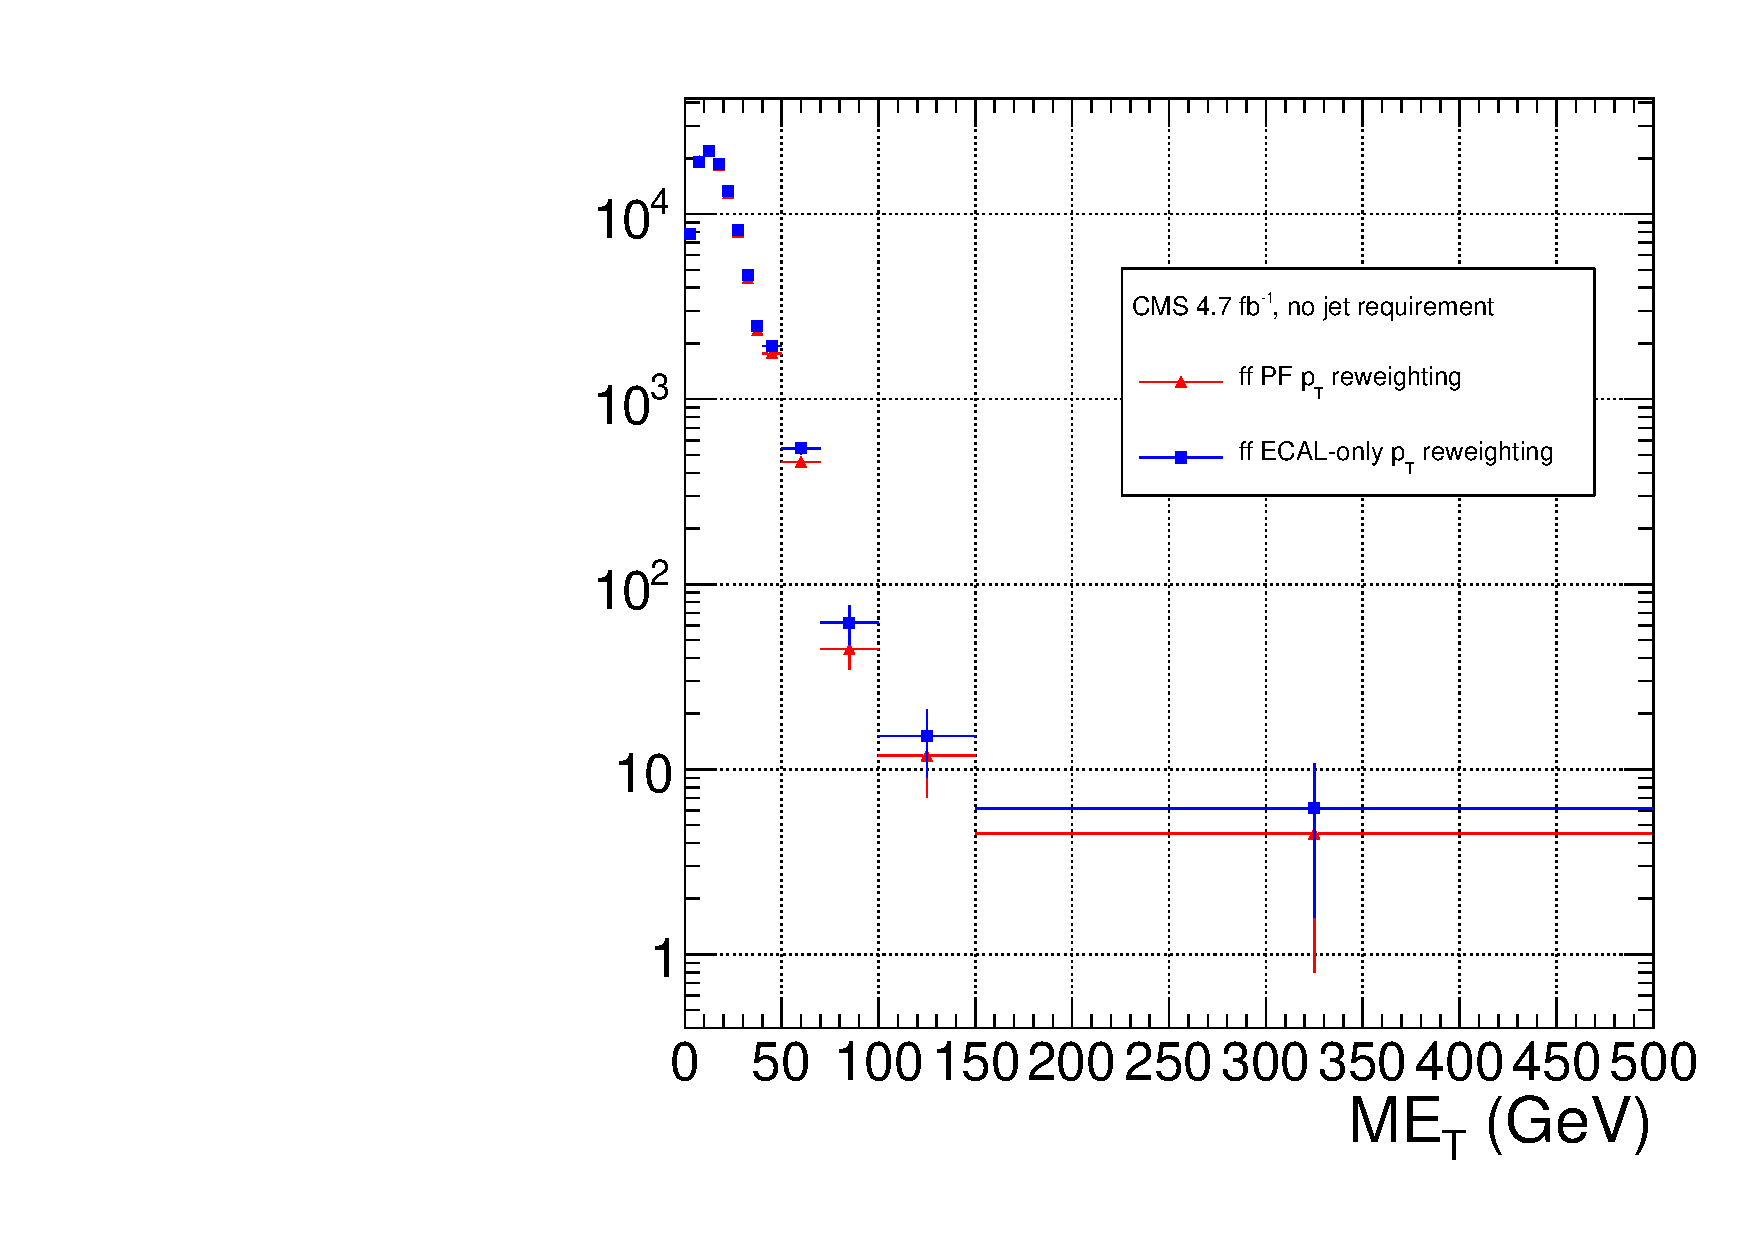
\includegraphics[scale=0.3]{ff_di-EM_vs_dijet_pT_reweighting}}
	\\
	\subfloat[Ratio of $ee$ to $\mathit{ff}$ \MET spectra.]{\label{fig:ee_over_ff_di-EM_vs_dijet_pT_reweighting}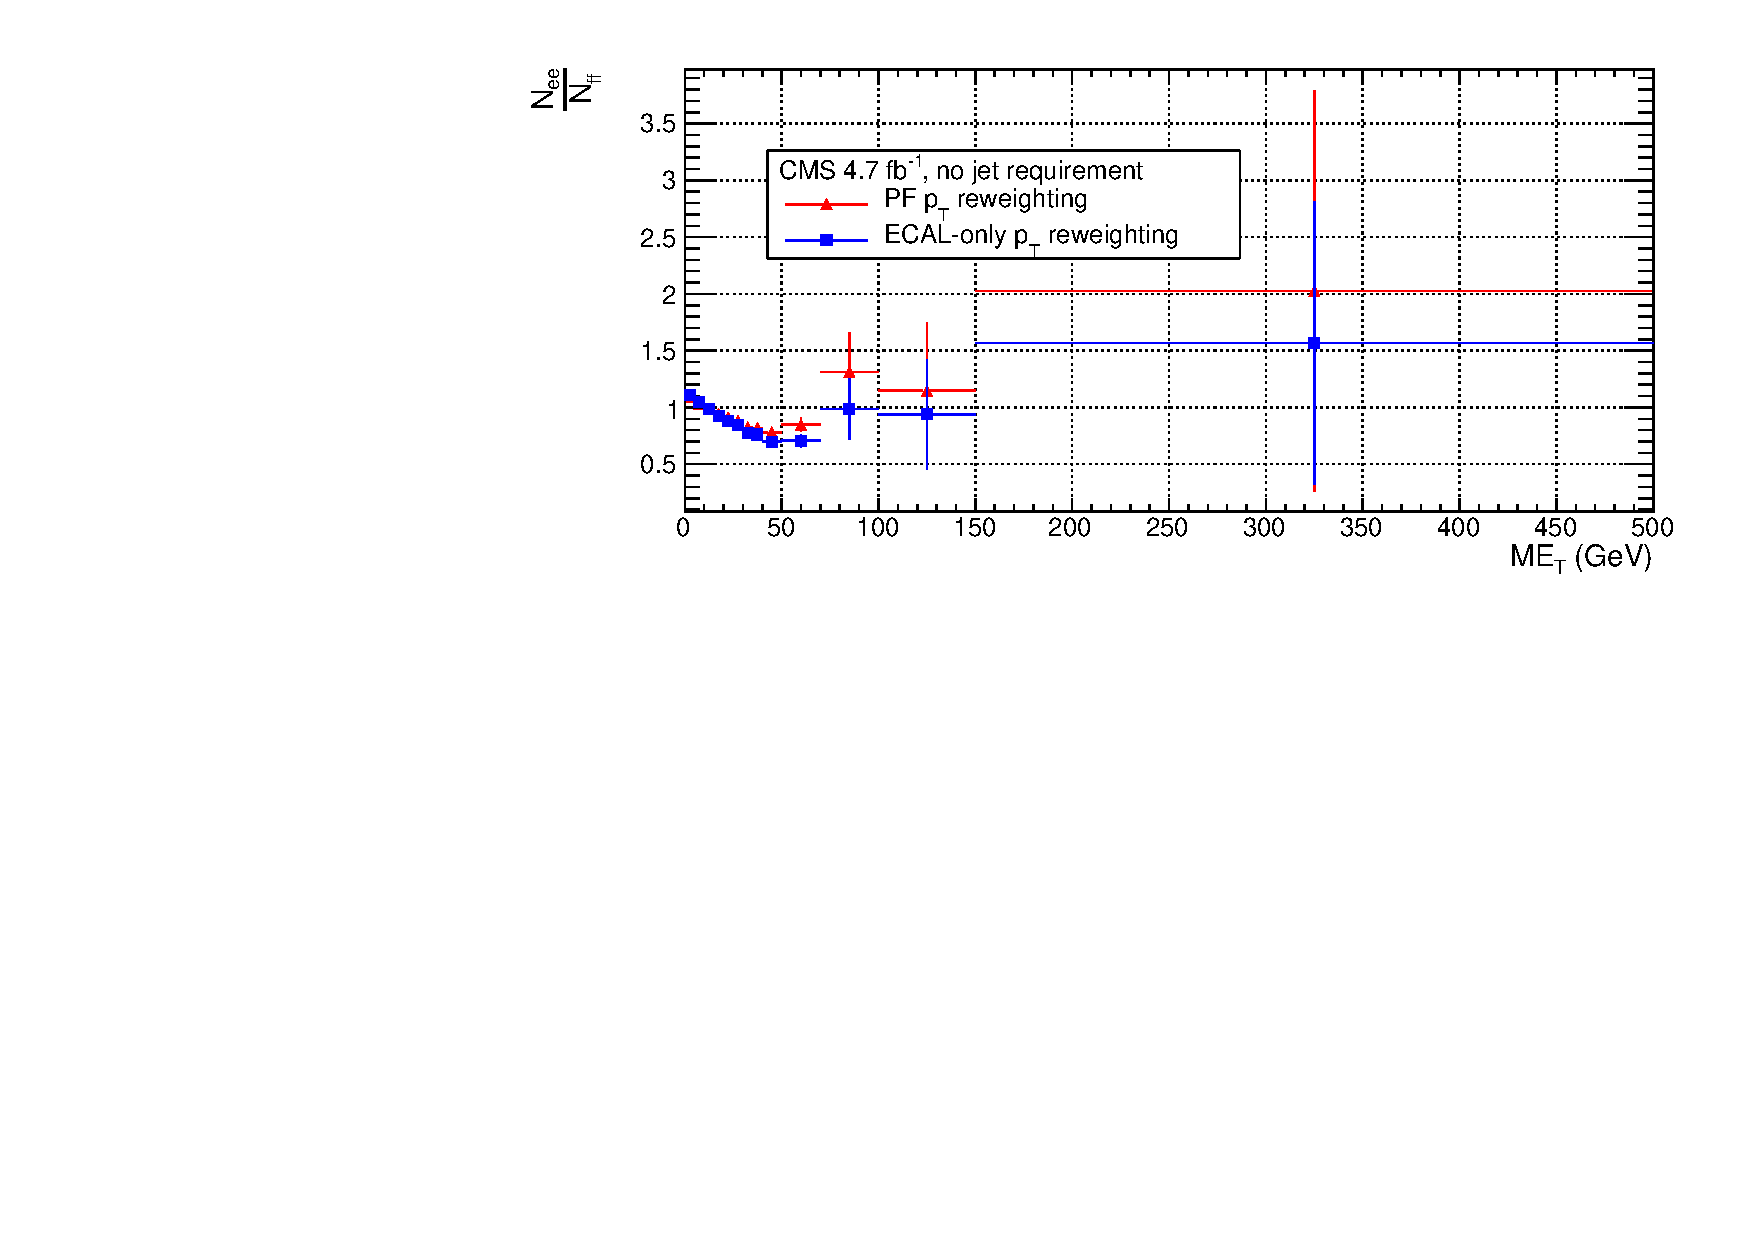
\includegraphics[scale=0.3]{ee_over_ff_di-EM_vs_dijet_pT_reweighting}}
	\hspace{1cm}
	\subfloat[Ratio of $ee$ to $\mathit{ff}$ \MET spectra, zoomed x-axis.]{\label{fig:ee_over_ff_di-EM_vs_dijet_pT_reweighting_zoom}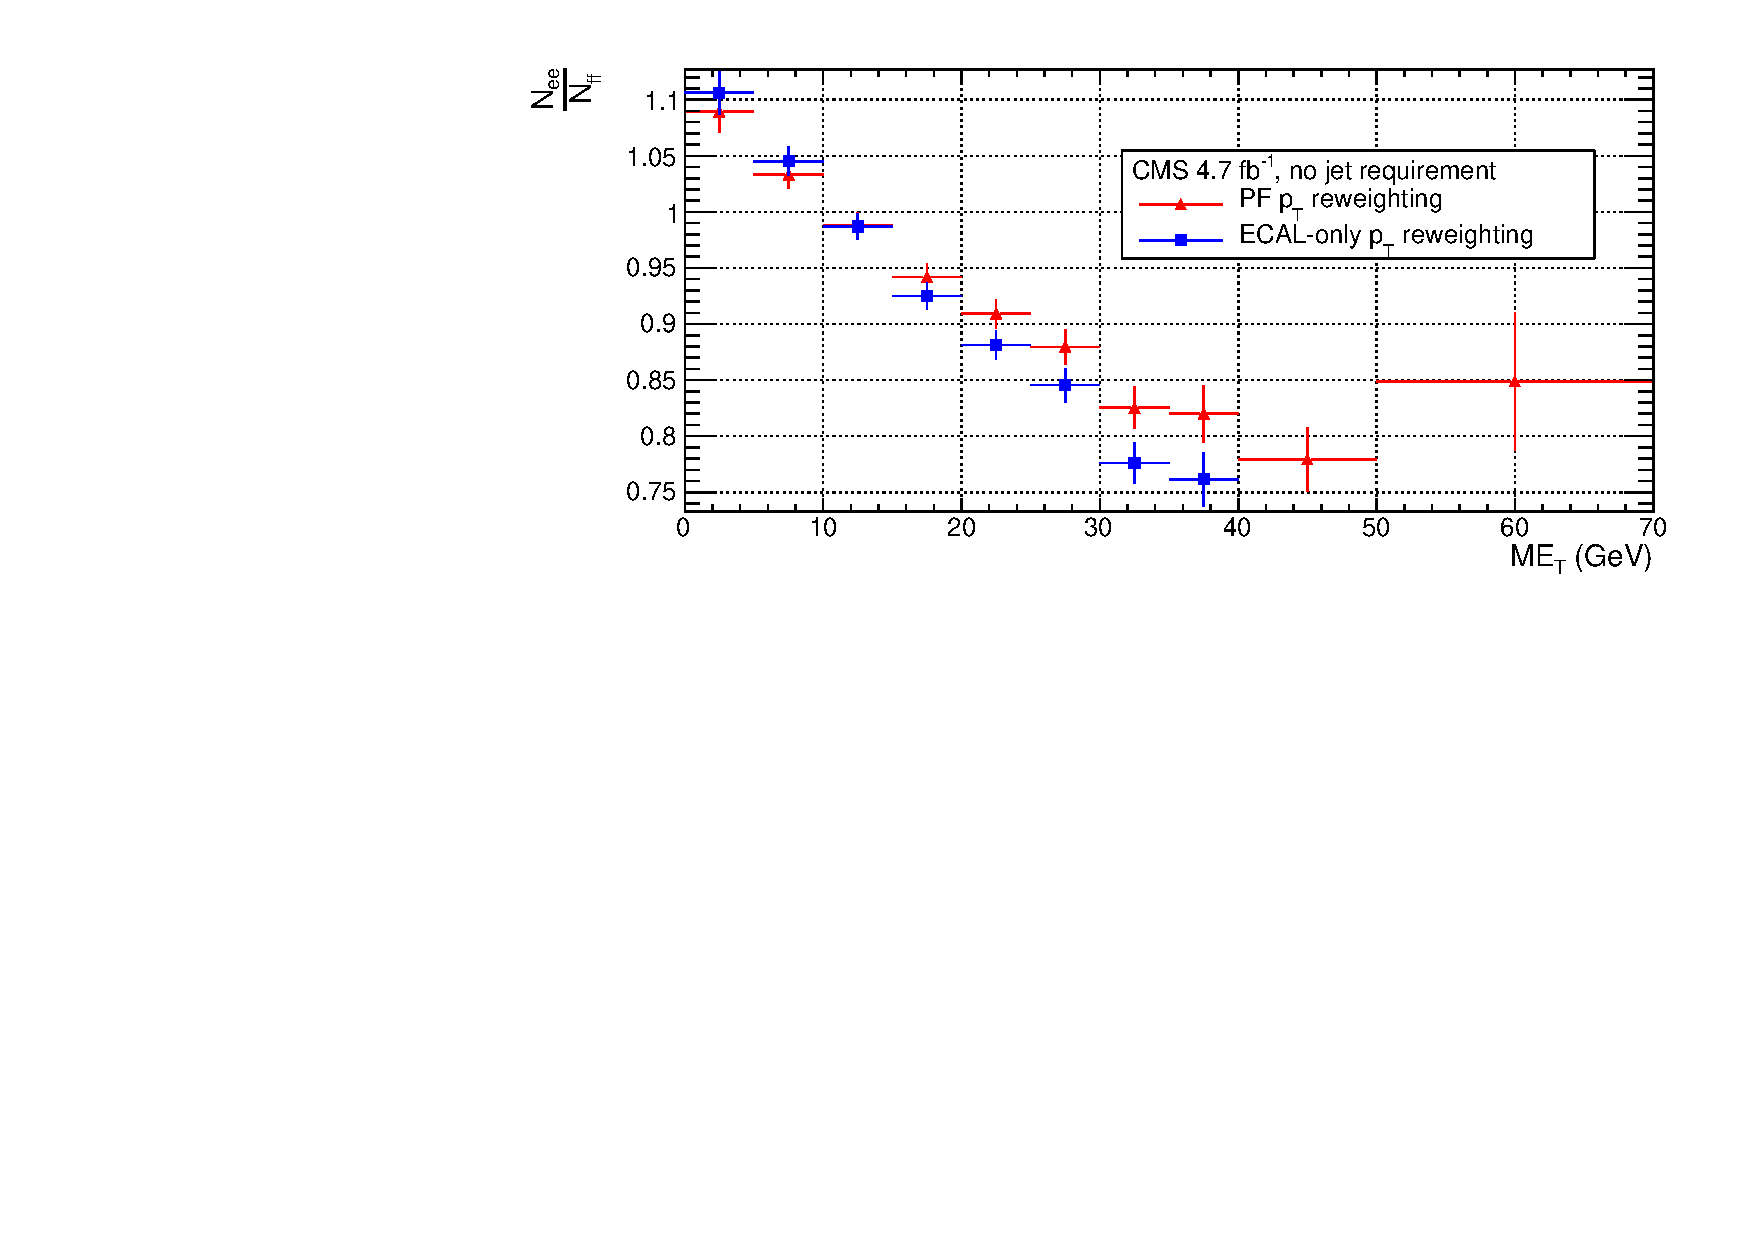
\includegraphics[scale=0.3]{ee_over_ff_di-EM_vs_dijet_pT_reweighting_zoom}}
	\caption{\MET spectra of the reweighted $ee$ (81 GeV $\leq m_{\mathrm{ee}} <$ 101 GeV) and $\mathit{ff}$ control samples.  Blue squares indicate reweighting using the ECAL-only $p_{T}$ estimate; red triangles indicate reweighting using the PF $p_{T}$ estimate.  The full reweighting and normalization procedure is employed, along with $ee$ sideband subtraction (discussed at the end of this section).  Error bars are statistical only.}
	\label{fig:ee_vs_ff_di-EM_vs_dijet_pT_reweighting}
\end{figure}

The control sample event weights are defined as

\begin{eqnarray}
w_{ij} &=& \frac{N_{\mathrm{control}}}{N_{\gamma\gamma}}\frac{N_{\gamma\gamma}^{ij}}{N_{\mathrm{control}}^{ij}}
\end{eqnarray}
%
where $i$ runs over the number of di-EM $p_{T}$ bins, $j$ runs over the number of jet bins, $N_{\mathrm{control}}$ is the total number of events in the control sample, $N_{\gamma\gamma}$ is the total number of events in the $\gamma\gamma$ sample, $N_{\gamma\gamma}^{ij}$ is the number of $\gamma\gamma$ events in the $i^{\mathrm{th}}$ di-EM $p_{T}$ bin and $j^{\mathrm{th}}$ jet bin, and $N_{\mathrm{control}}^{ij}$ is the number of control sample events in the $i^{\mathrm{th}}$ di-EM $p_{T}$ bin and $j^{\mathrm{th}}$ jet bin.  The effect of the reweighting is more significant for the $ee$ sample than for the $\mathit{ff}$ sample, as shown in Figure~\ref{fig:reweighting_vs_no_reweighting}.

%include ee/gg and ff/gg agreement?
%include similar figures for MC?
\begin{figure}
	\centering
	\subfloat[$ee$ \MET spectra.]{\label{fig:ee_dijet_pT_and_Nj_vs_no_reweighting}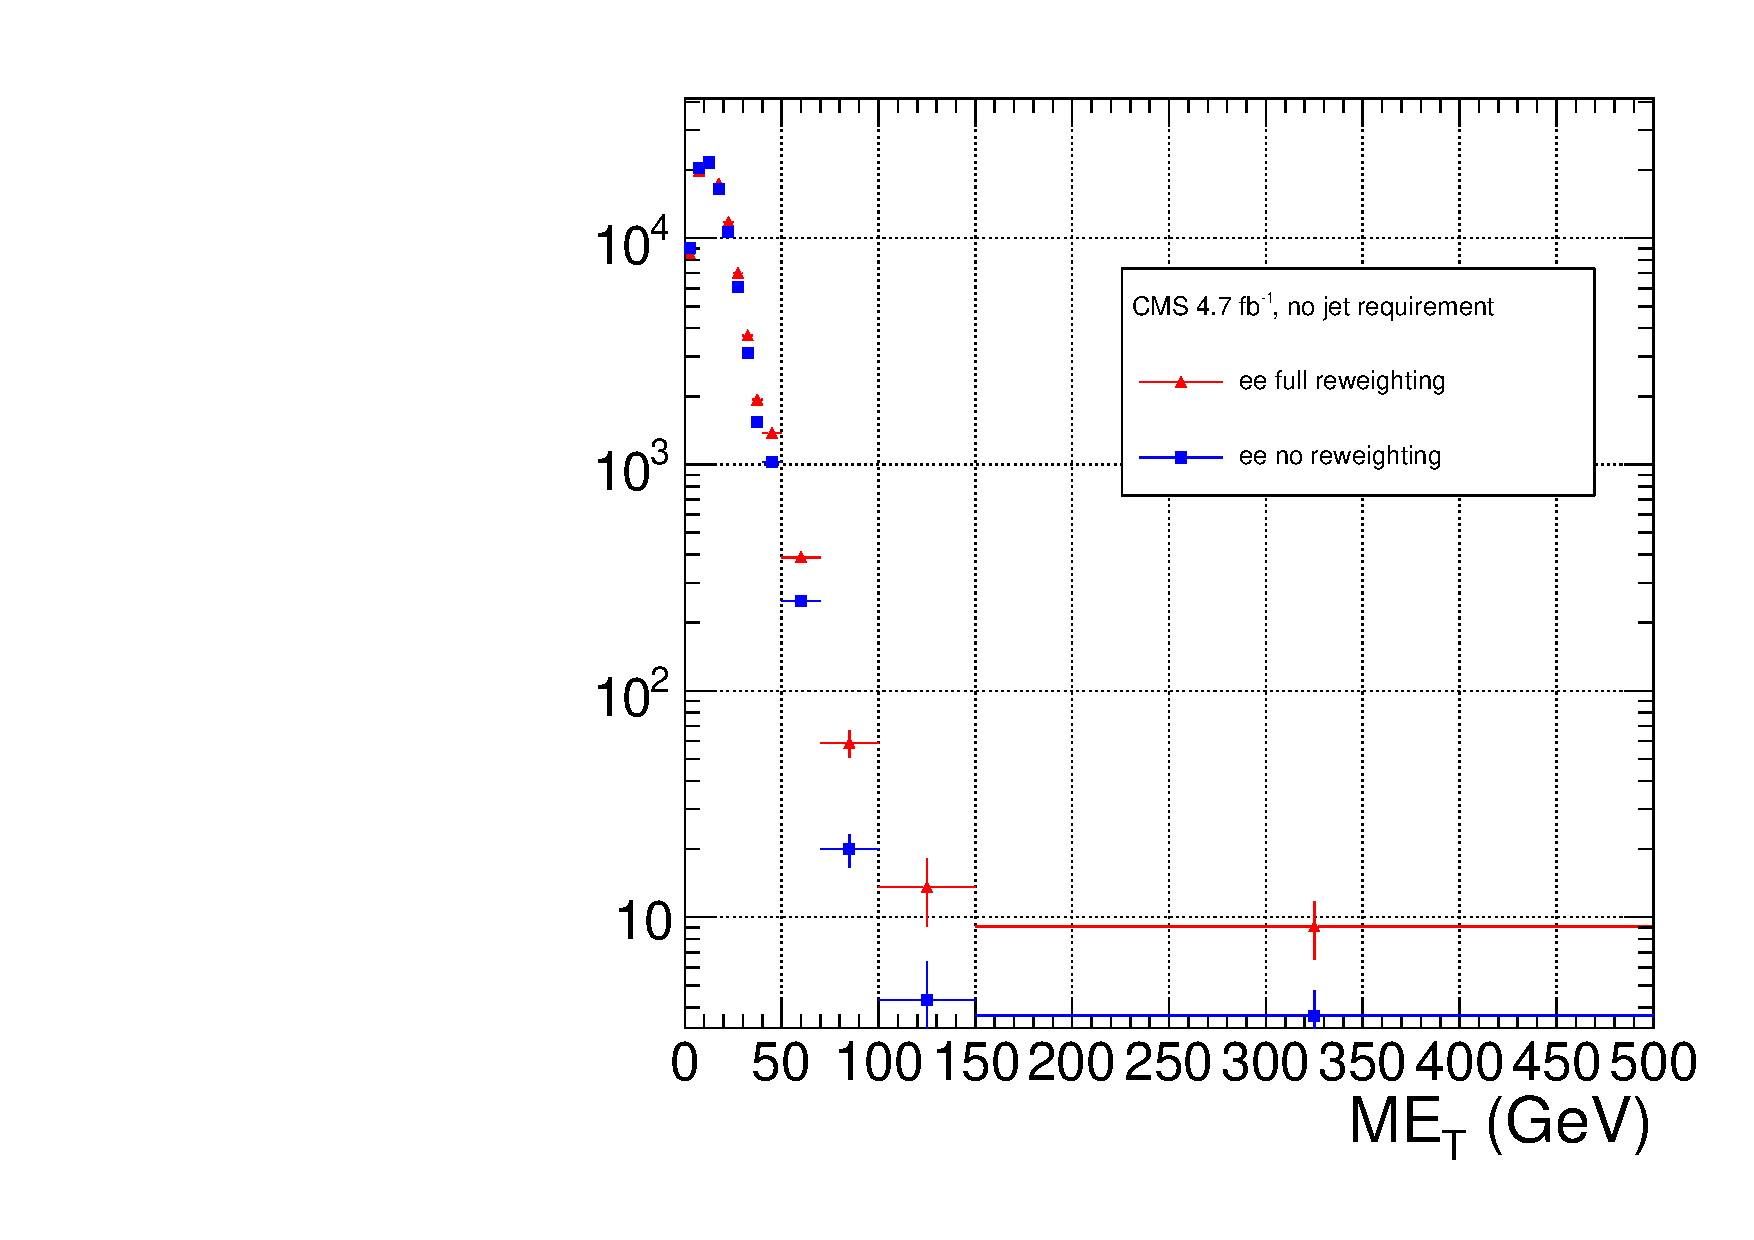
\includegraphics[scale=0.3]{ee_dijet_pT_and_Nj_vs_no_reweighting}}
	\hspace{1cm}
	\subfloat[$\mathit{ff}$ \MET spectra.]{\label{fig:ff_dijet_pT_and_Nj_vs_no_reweighting}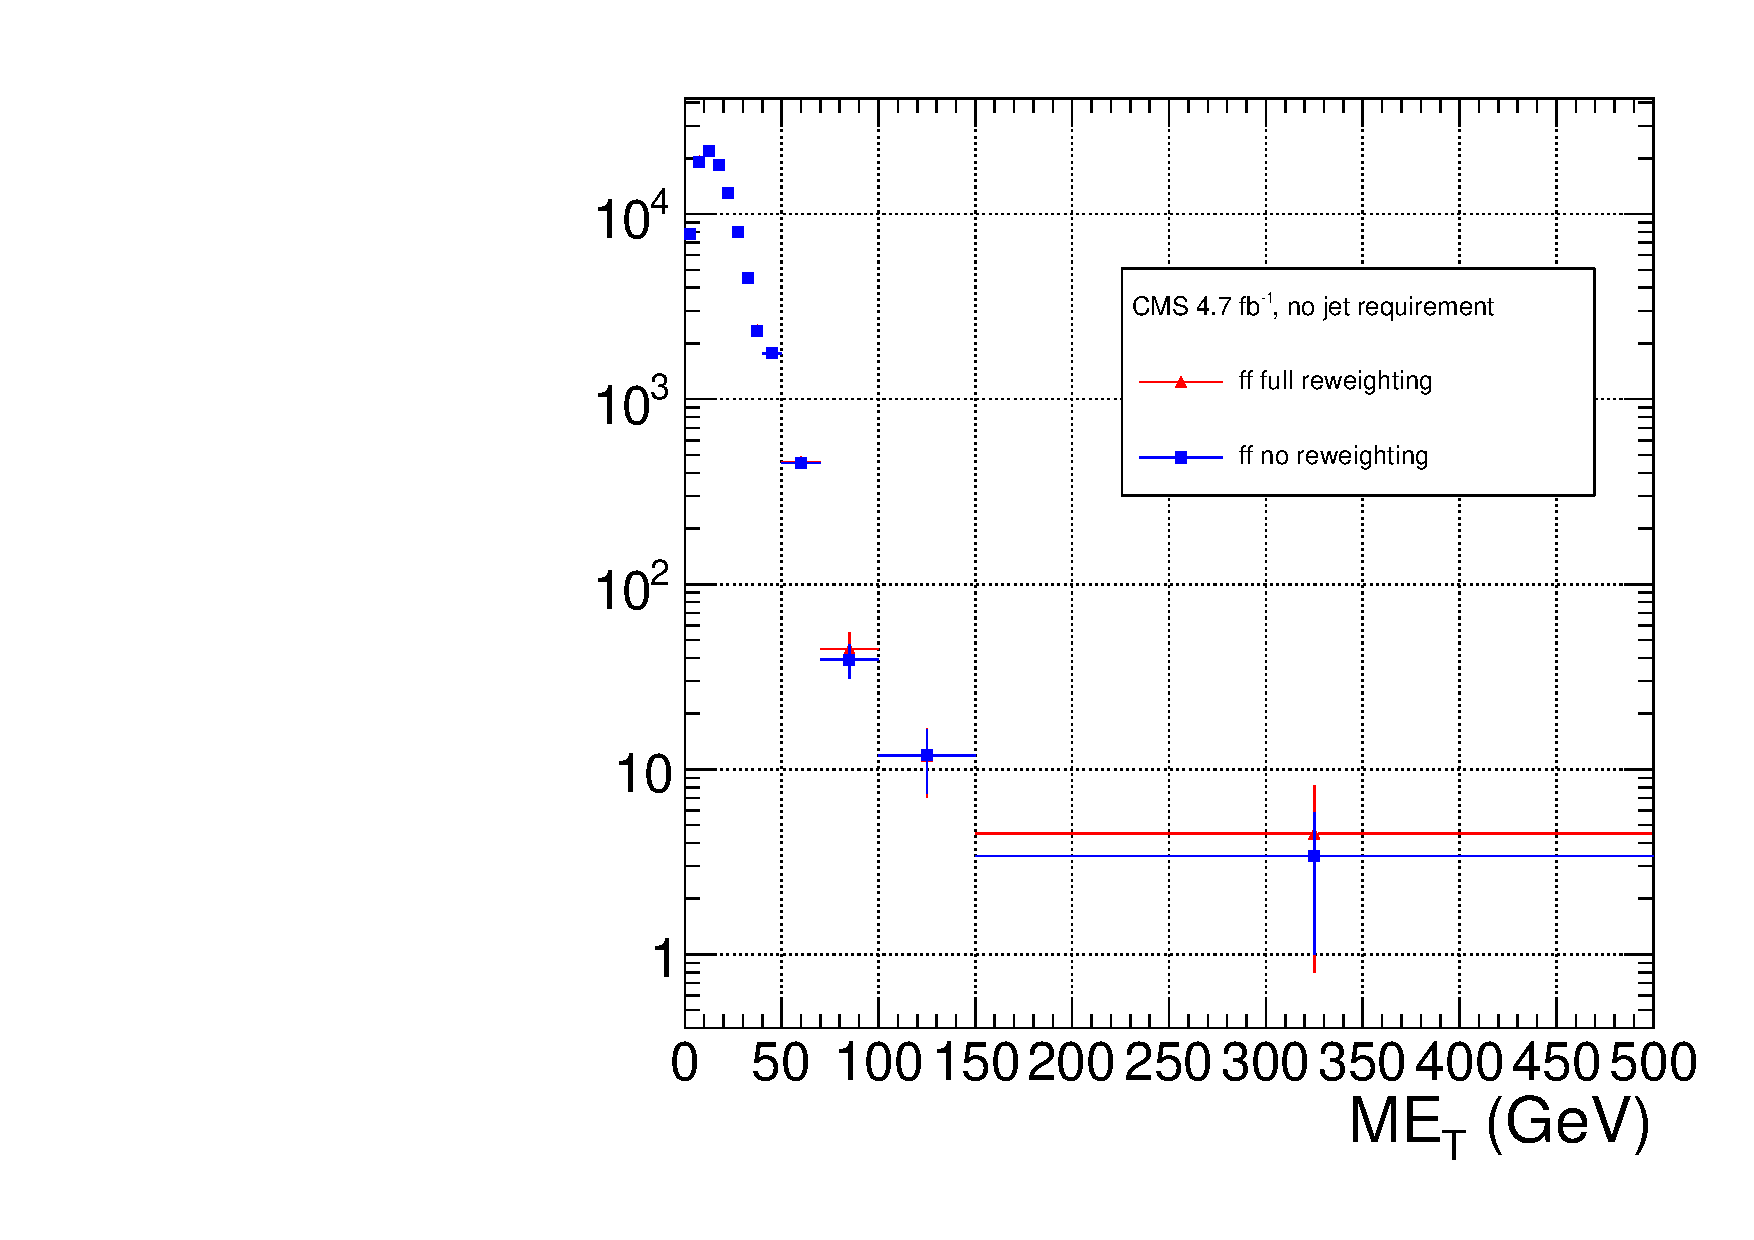
\includegraphics[scale=0.3]{ff_dijet_pT_and_Nj_vs_no_reweighting}}
	\\
	\subfloat[Ratio of $ee$ to $\mathit{ff}$ \MET spectra.]{\label{fig:ee_over_ff_dijet_pT_and_Nj_vs_no_reweighting}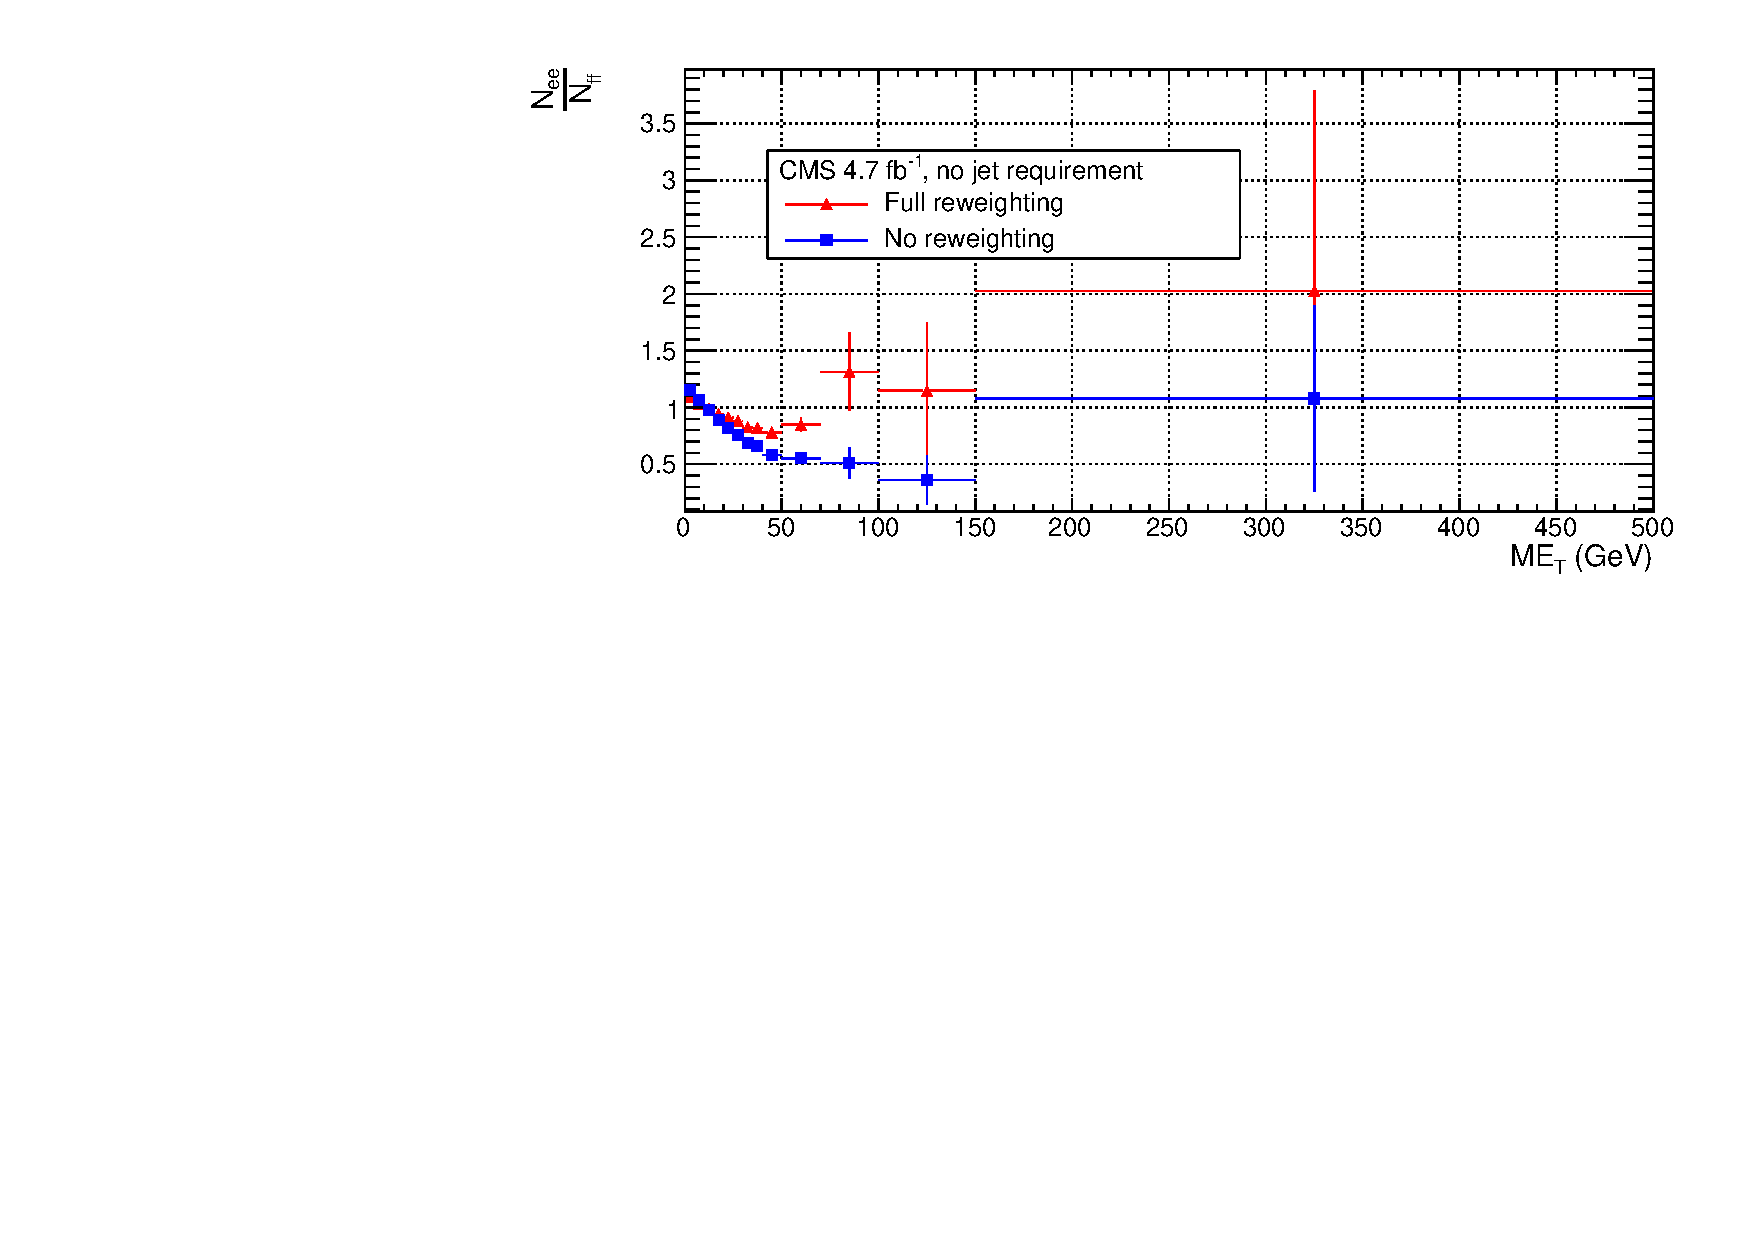
\includegraphics[scale=0.3]{ee_over_ff_dijet_pT_and_Nj_vs_no_reweighting}}
	\hspace{1cm}
	\subfloat[Ratio of $ee$ to $\mathit{ff}$ \MET spectra, zoomed x-axis.]{\label{fig:ee_over_ff_dijet_pT_and_Nj_vs_no_reweighting_zoom}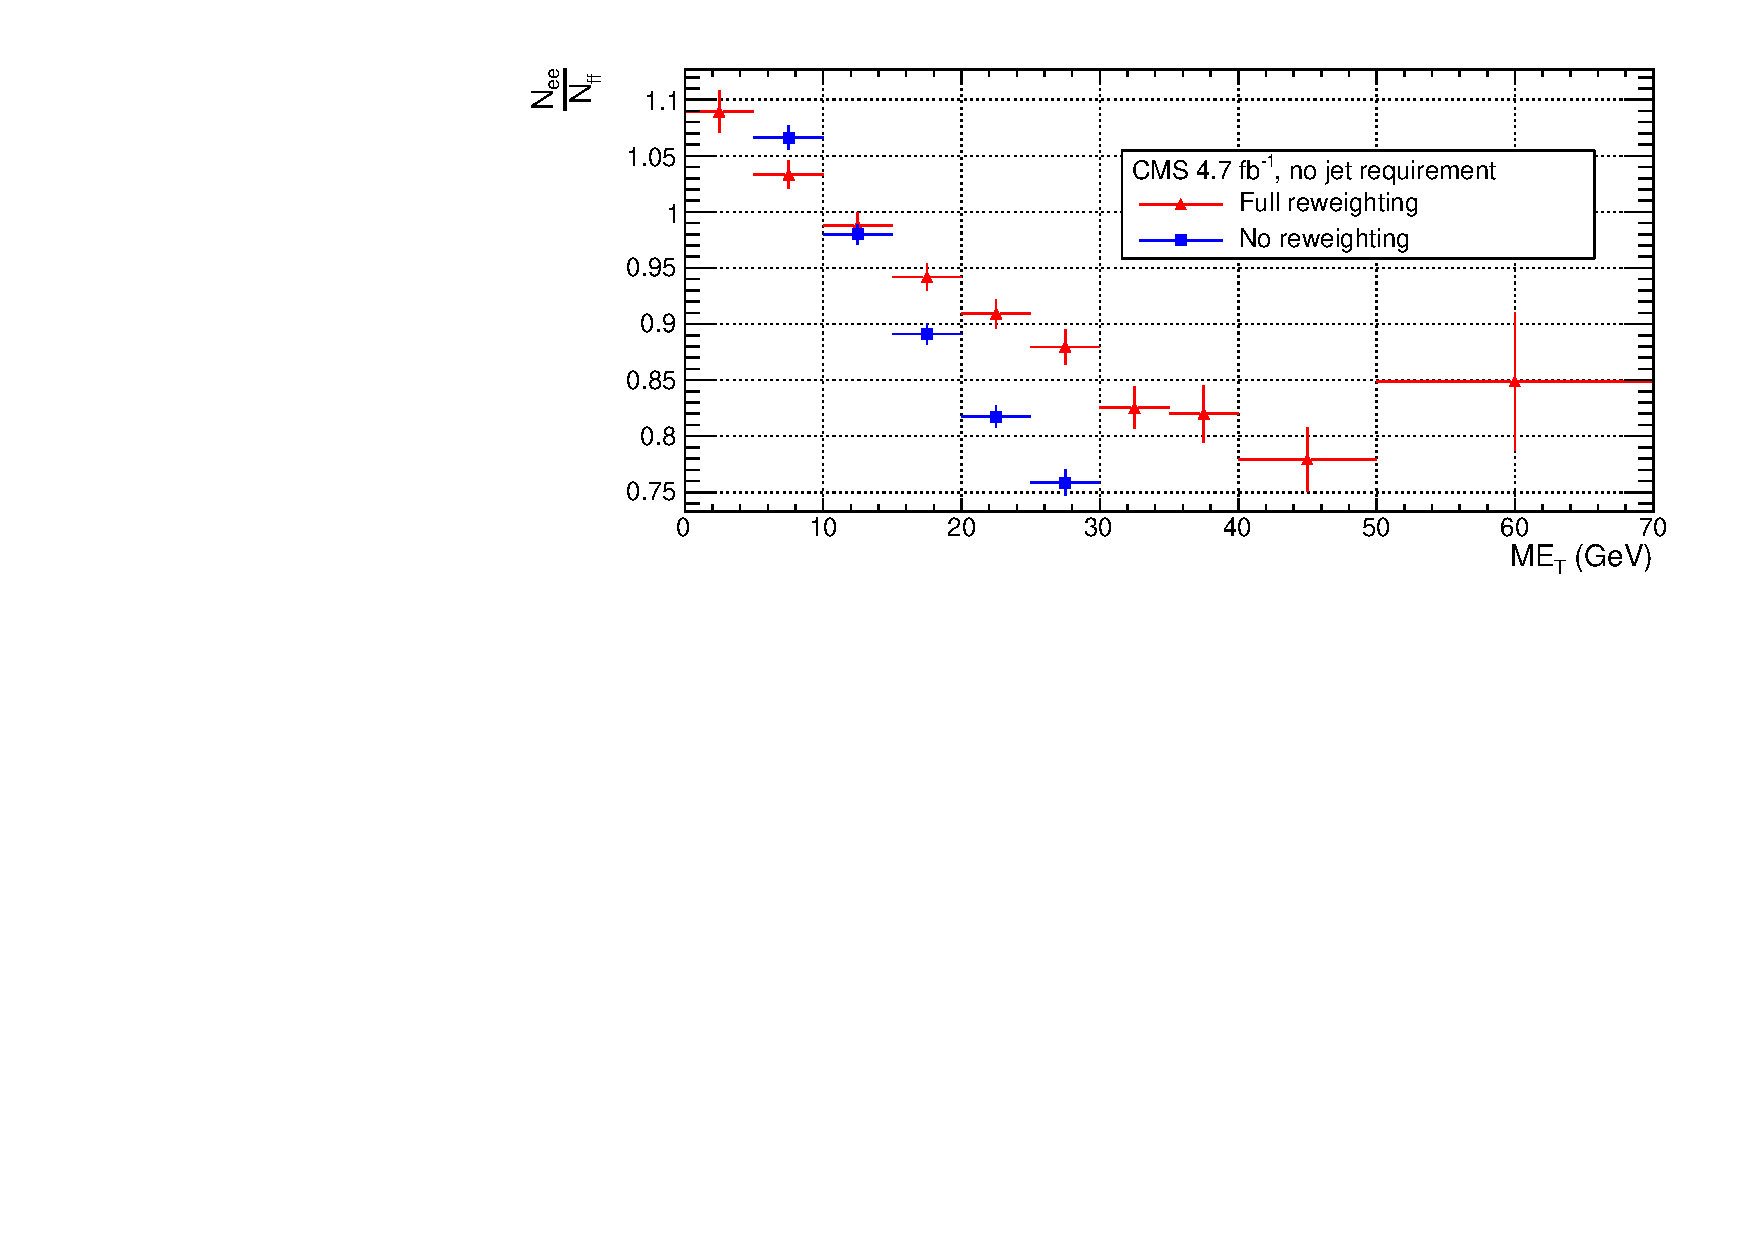
\includegraphics[scale=0.3]{ee_over_ff_dijet_pT_and_Nj_vs_no_reweighting_zoom}}
	\caption{\MET spectra of the $ee$ (81 GeV $\leq m_{\mathrm{ee}} <$ 101 GeV) and $\mathit{ff}$ control samples.  Red triangles indicate full di-EM $p_{T}$ + number of jets reweighting; blue squares indicate no reweighting.  PF $p_{T}$ (cf. p.~\pageref{fig:ET_bias_vs_EMF}) is used to calculate the di-EM $p_{T}$.  The full normalization procedure is employed, along with $ee$ sideband subtraction (discussed at the end of this section).  Error bars are statistical only.}
	\label{fig:reweighting_vs_no_reweighting}
\end{figure}

The $ee$ sample contains a non-negligible background of $t\bar{t}$ events in which both $W$ bosons decay to electrons.  These events have significant real \MET from the two neutrinos (unlike the $\gamma\gamma$ events), and therefore inflate the background estimate at high \MET.  In order to remove the $t\bar{t}$ contribution from the $ee$ sample, a sideband subtraction method is employed.

Only events in the $ee$ sample with 81 GeV $\leq m_{\mathrm{ee}} <$ 101 GeV, where $m_{\mathrm{ee}}$ is the di-electron invariant mass, are used in the QCD background estimate.  This choice maximizes the ratio of $Z$ signal to background.  The sidebands used to estimate the background contribution within the $Z$ window are defined such that 71 GeV $\leq m_{\mathrm{ee}} <$ 81 GeV and 101 GeV $\leq m_{\mathrm{ee}} <$ 111 GeV.

The full reweighting procedure is applied to the $Z$ signal region and the two sideband regions independently.  Only $Z$ signal events are used in the calculation of the di-EM $p_{T}$ weights for the $Z$ signal region, and likewise only the events within a given sideband region are used in the calculation of the weights for that region.  Assuming a constant $t\bar{t}$ background shape, the resulting reweighted sideband \MET distributions are added together and subtracted from the reweighted $Z$ signal \MET distribution.  The sideband subtracted $Z$ signal \MET distribution is then normalized as discussed in Secs.~\ref{sec:Outline of the Procedure} and~\ref{sec:Normalization}.  The statistical and reweighting error from the sideband regions is propagated to the error on the final $ee$ QCD \MET estimate.

The di-EM $p_{T}$ weights for the two $ee$ sideband regions are shown in Figure~\ref{fig:ee_sideband_dijet_pT_weights}.  The overall scale of the weights, as well as the trend with di-EM $p_{T}$, is similar for the two regions (except at high di-EM $p_{T}$, where the statistics are poor anyway).  Figure~\ref{fig:all_ee_MET_spectra} shows the \MET spectra for the two sideband regions and the $Z$ signal region after subtraction.  The shapes of the spectra indicate that the high-\MET $t\bar{t}$ tail, present in the sideband distributions, was successfully subtracted from the $Z$ signal distribution.

\begin{figure}
	\centering
	\subfloat[71 GeV $\leq m_{\mathrm{ee}} <$ 81 GeV, 0 jets.]{\label{fig:eeLowSideband_0_jet_dijet_pT_weights}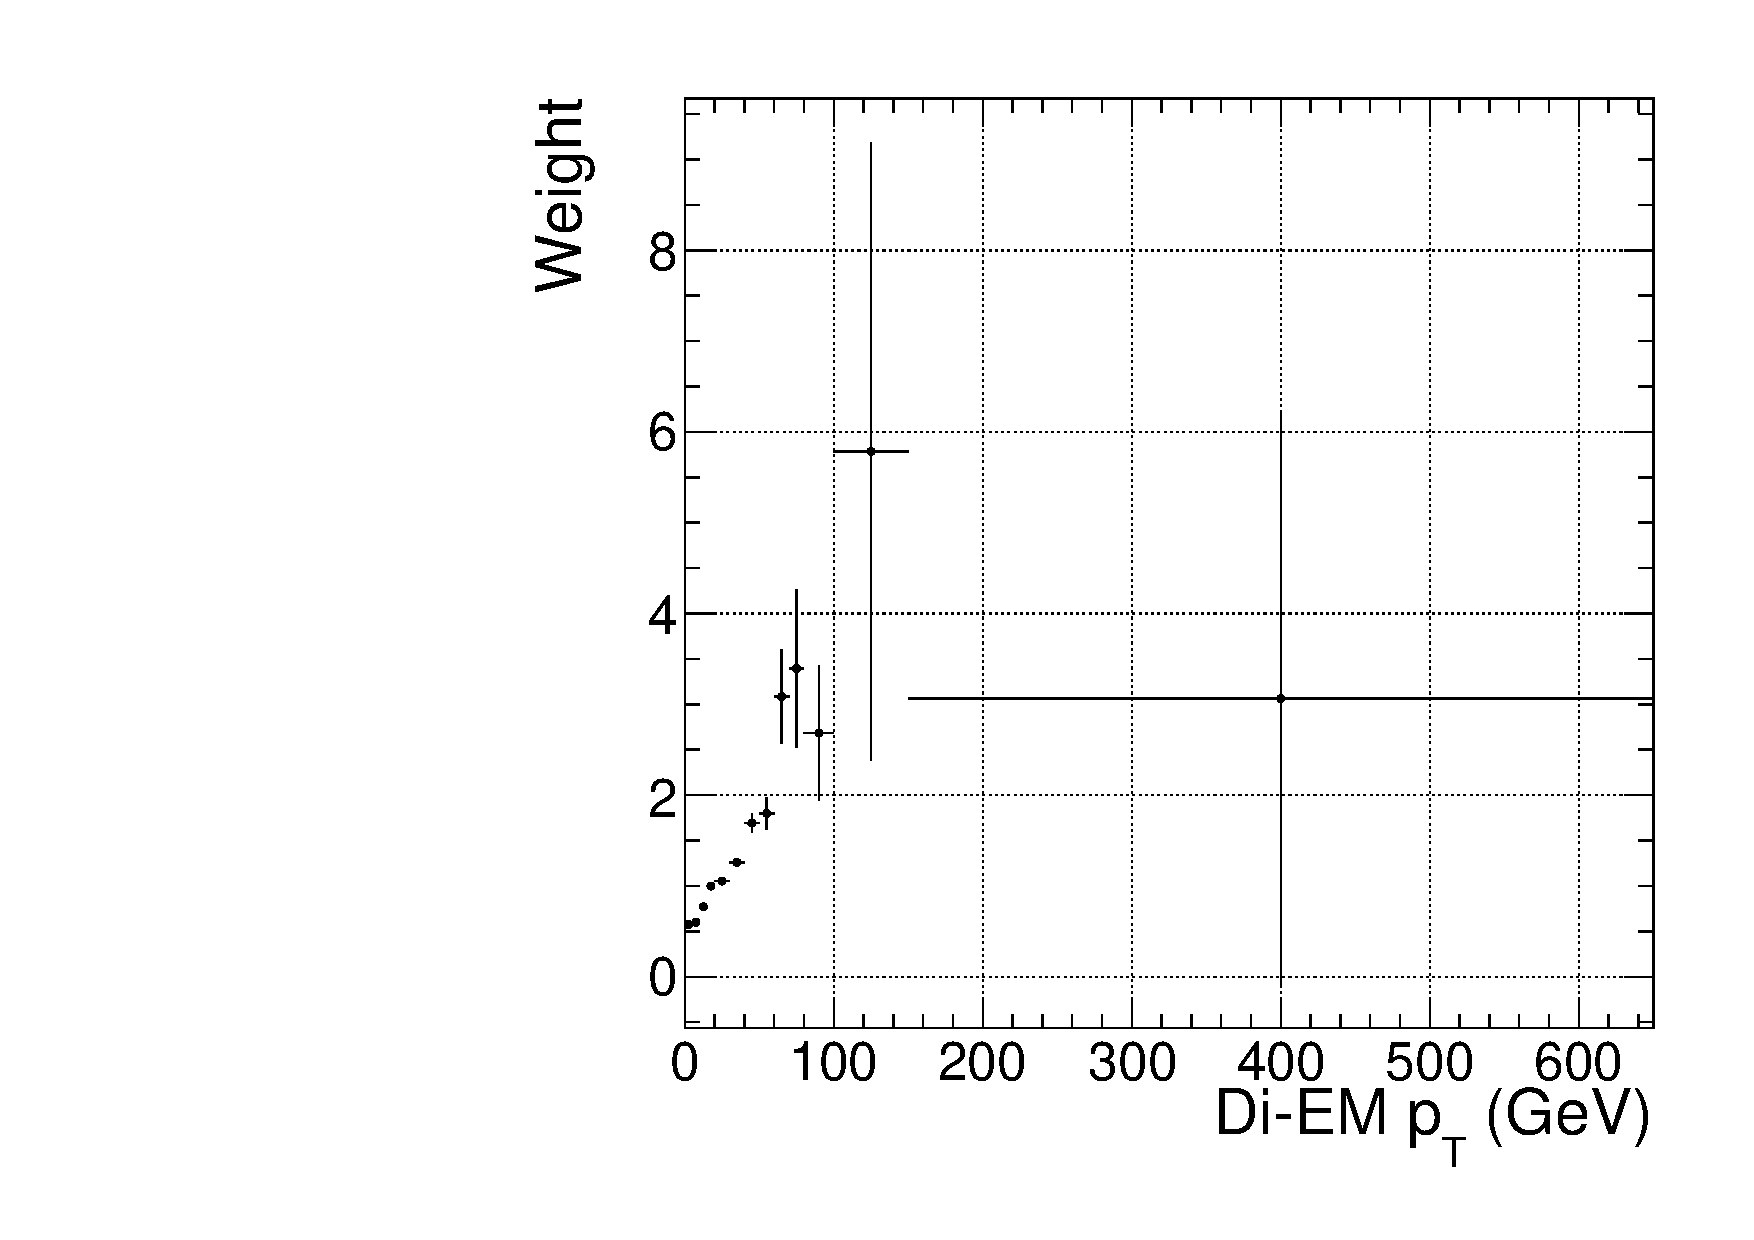
\includegraphics[scale=0.2]{eeLowSideband_0_jet_dijet_pT_weights}}
	\hspace{1cm}
	\subfloat[71 GeV $\leq m_{\mathrm{ee}} <$ 81 GeV, 1 jet.]{\label{fig:eeLowSideband_1_jet_dijet_pT_weights}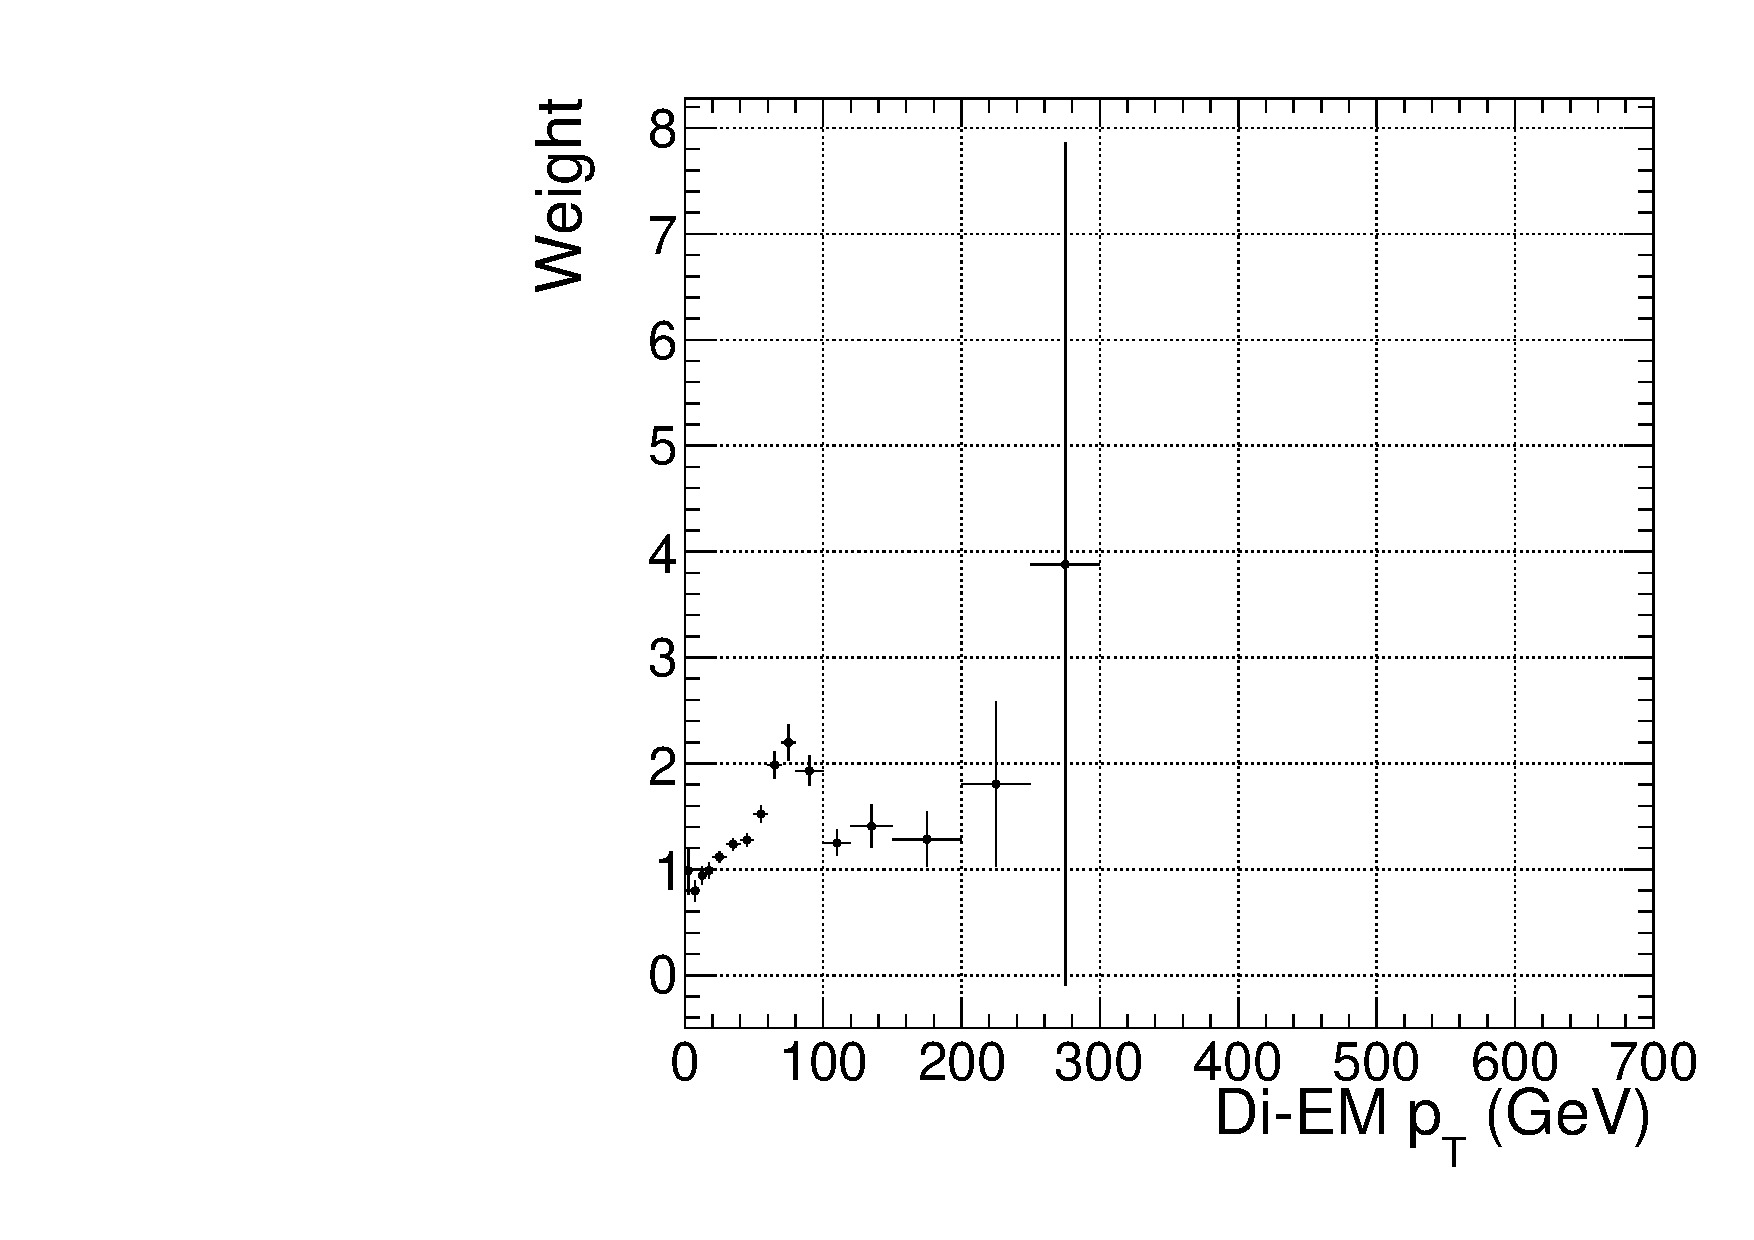
\includegraphics[scale=0.2]{eeLowSideband_1_jet_dijet_pT_weights}}
	\hspace{1cm}
	\subfloat[71 GeV $\leq m_{\mathrm{ee}} <$ 81 GeV, $\geq$ 2 jets.]{\label{fig:eeLowSideband_2_jet_dijet_pT_weights}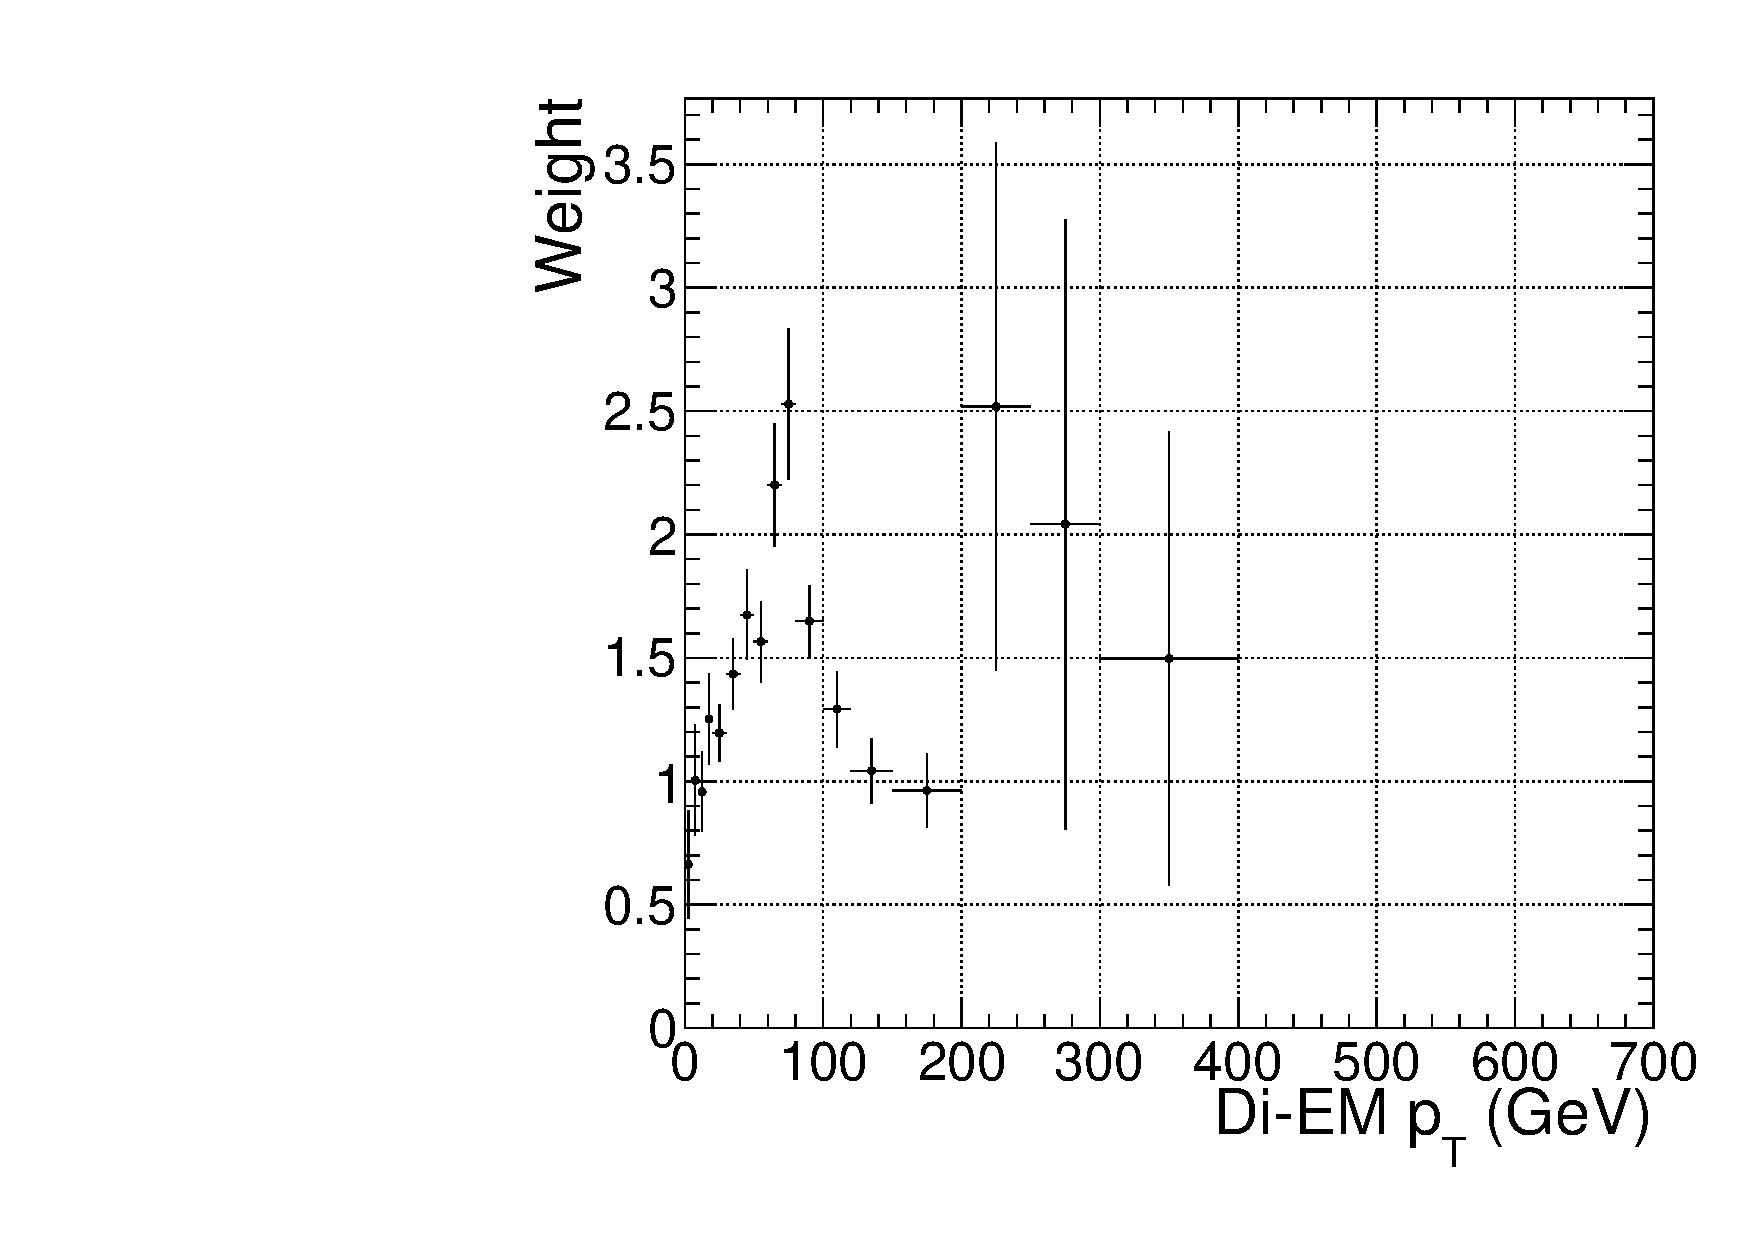
\includegraphics[scale=0.2]{eeLowSideband_2_jet_dijet_pT_weights}}
	\\
	\subfloat[101 GeV $\leq m_{\mathrm{ee}} <$ 111 GeV, 0 jets.]{\label{fig:eeHighSideband_0_jet_dijet_pT_weights}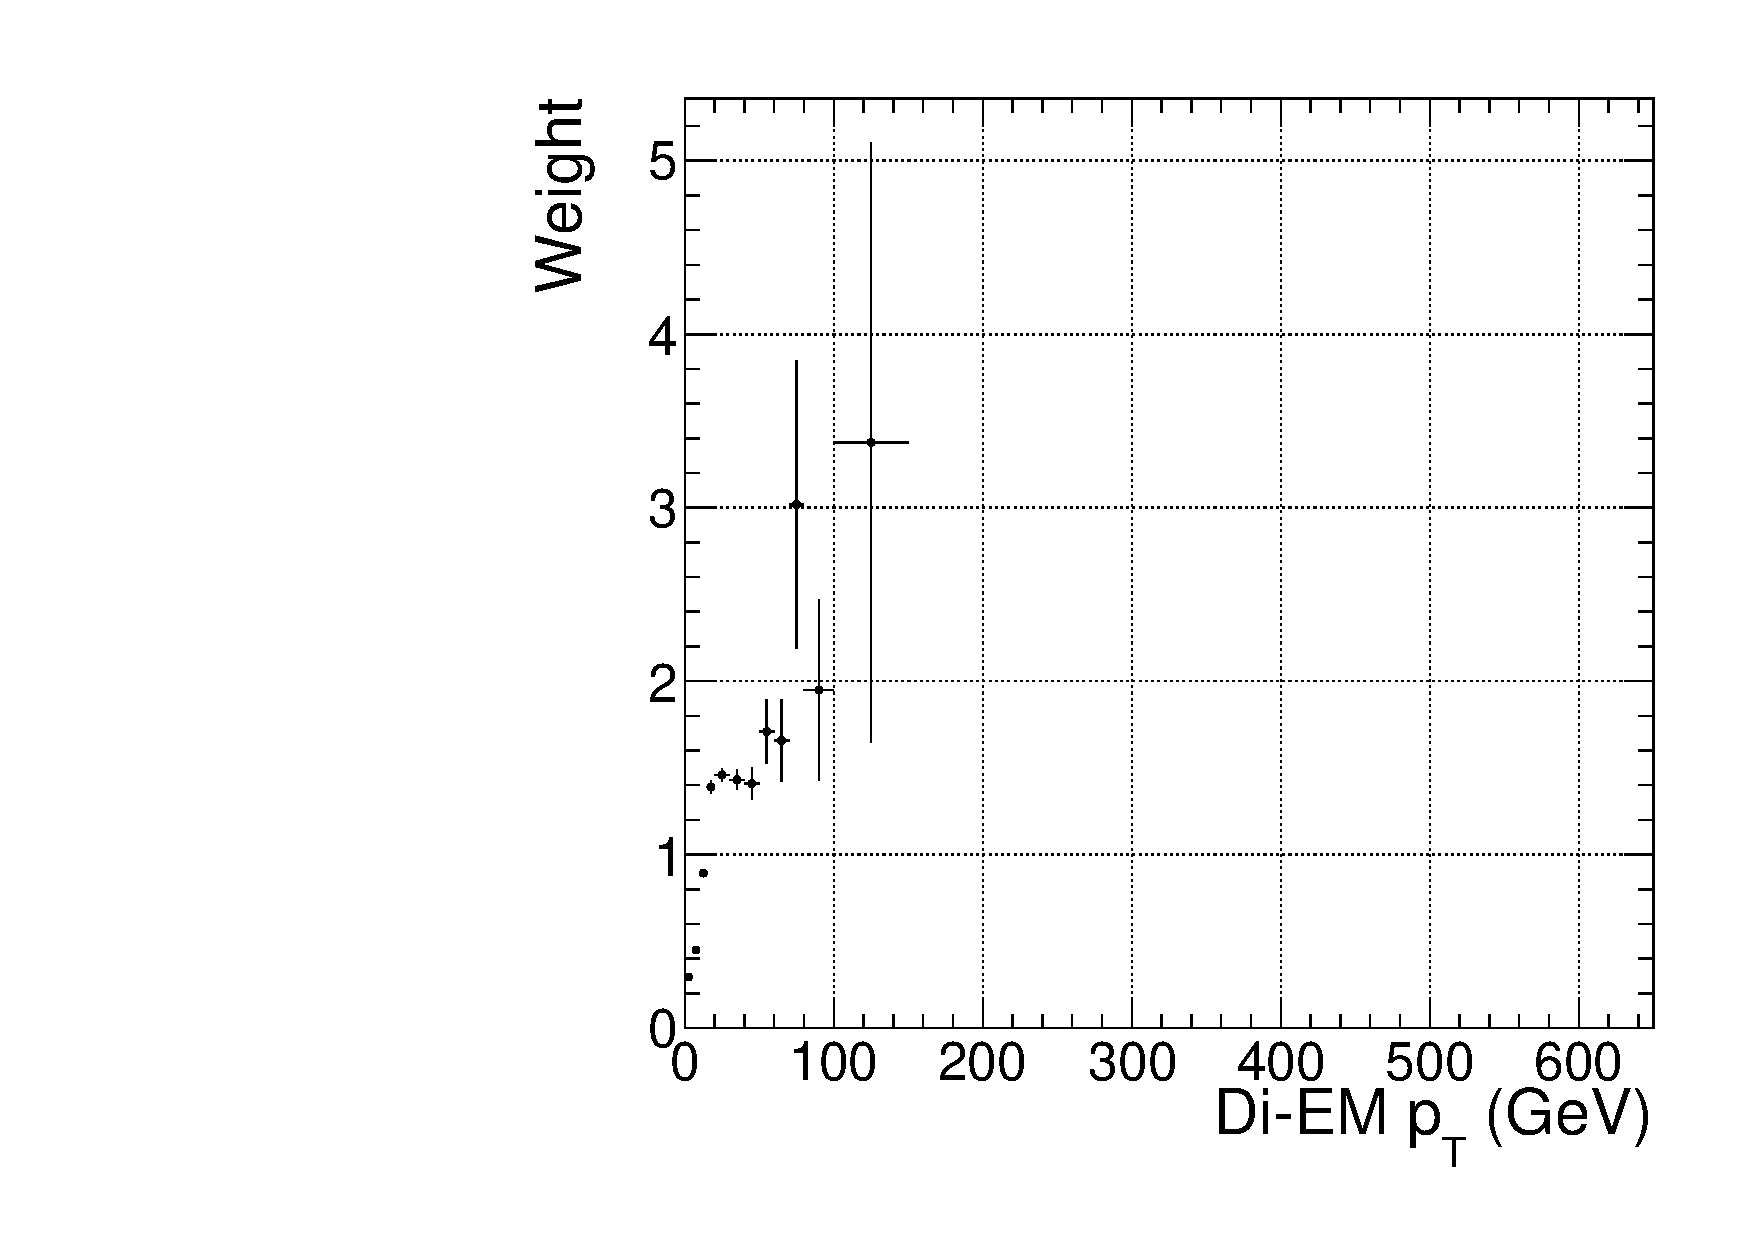
\includegraphics[scale=0.2]{eeHighSideband_0_jet_dijet_pT_weights}}
	\hspace{1cm}
	\subfloat[101 GeV $\leq m_{\mathrm{ee}} <$ 111 GeV, 1 jet.]{\label{fig:eeHighSideband_1_jet_dijet_pT_weights}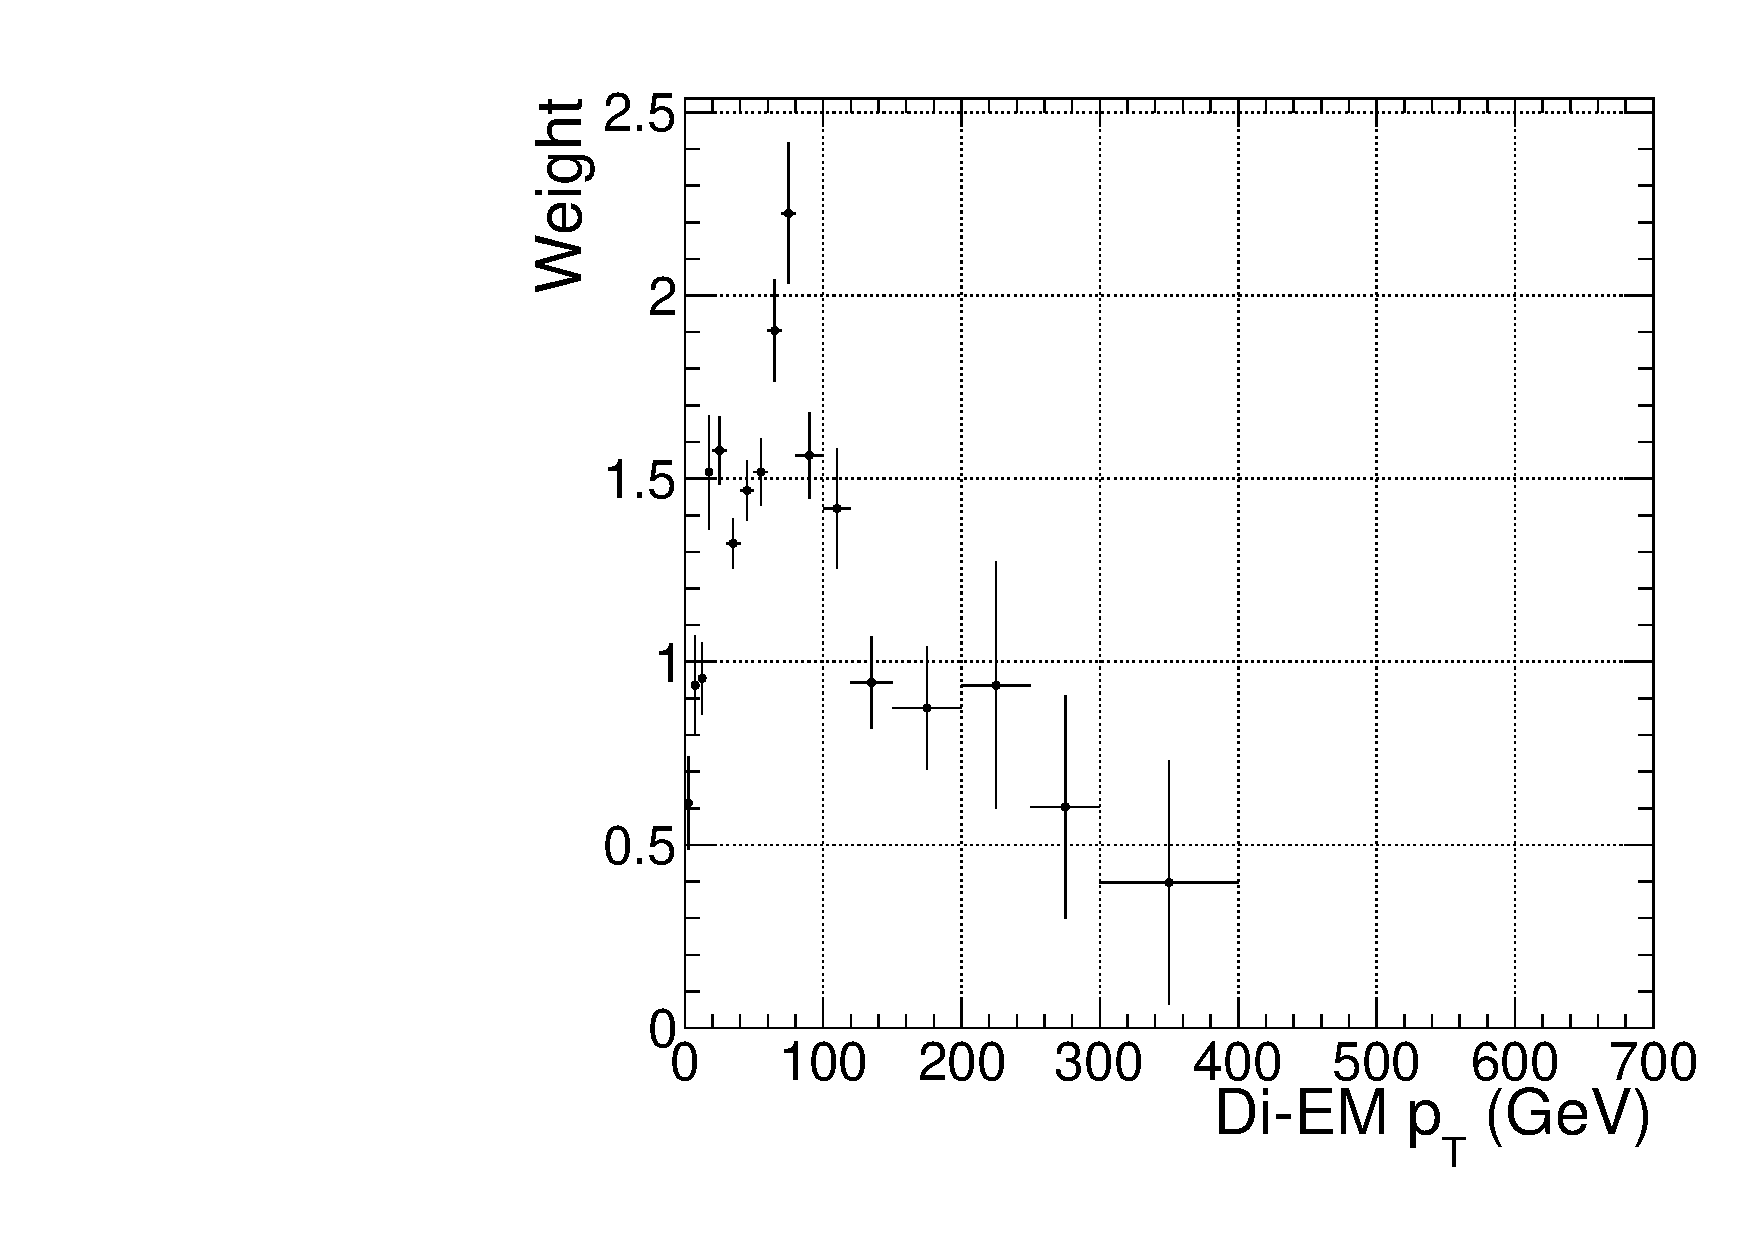
\includegraphics[scale=0.2]{eeHighSideband_1_jet_dijet_pT_weights}}
	\hspace{1cm}
	\subfloat[101 GeV $\leq m_{\mathrm{ee}} <$ 111 GeV, $\geq$ 2 jets.]{\label{fig:eeHighSideband_2_jet_dijet_pT_weights}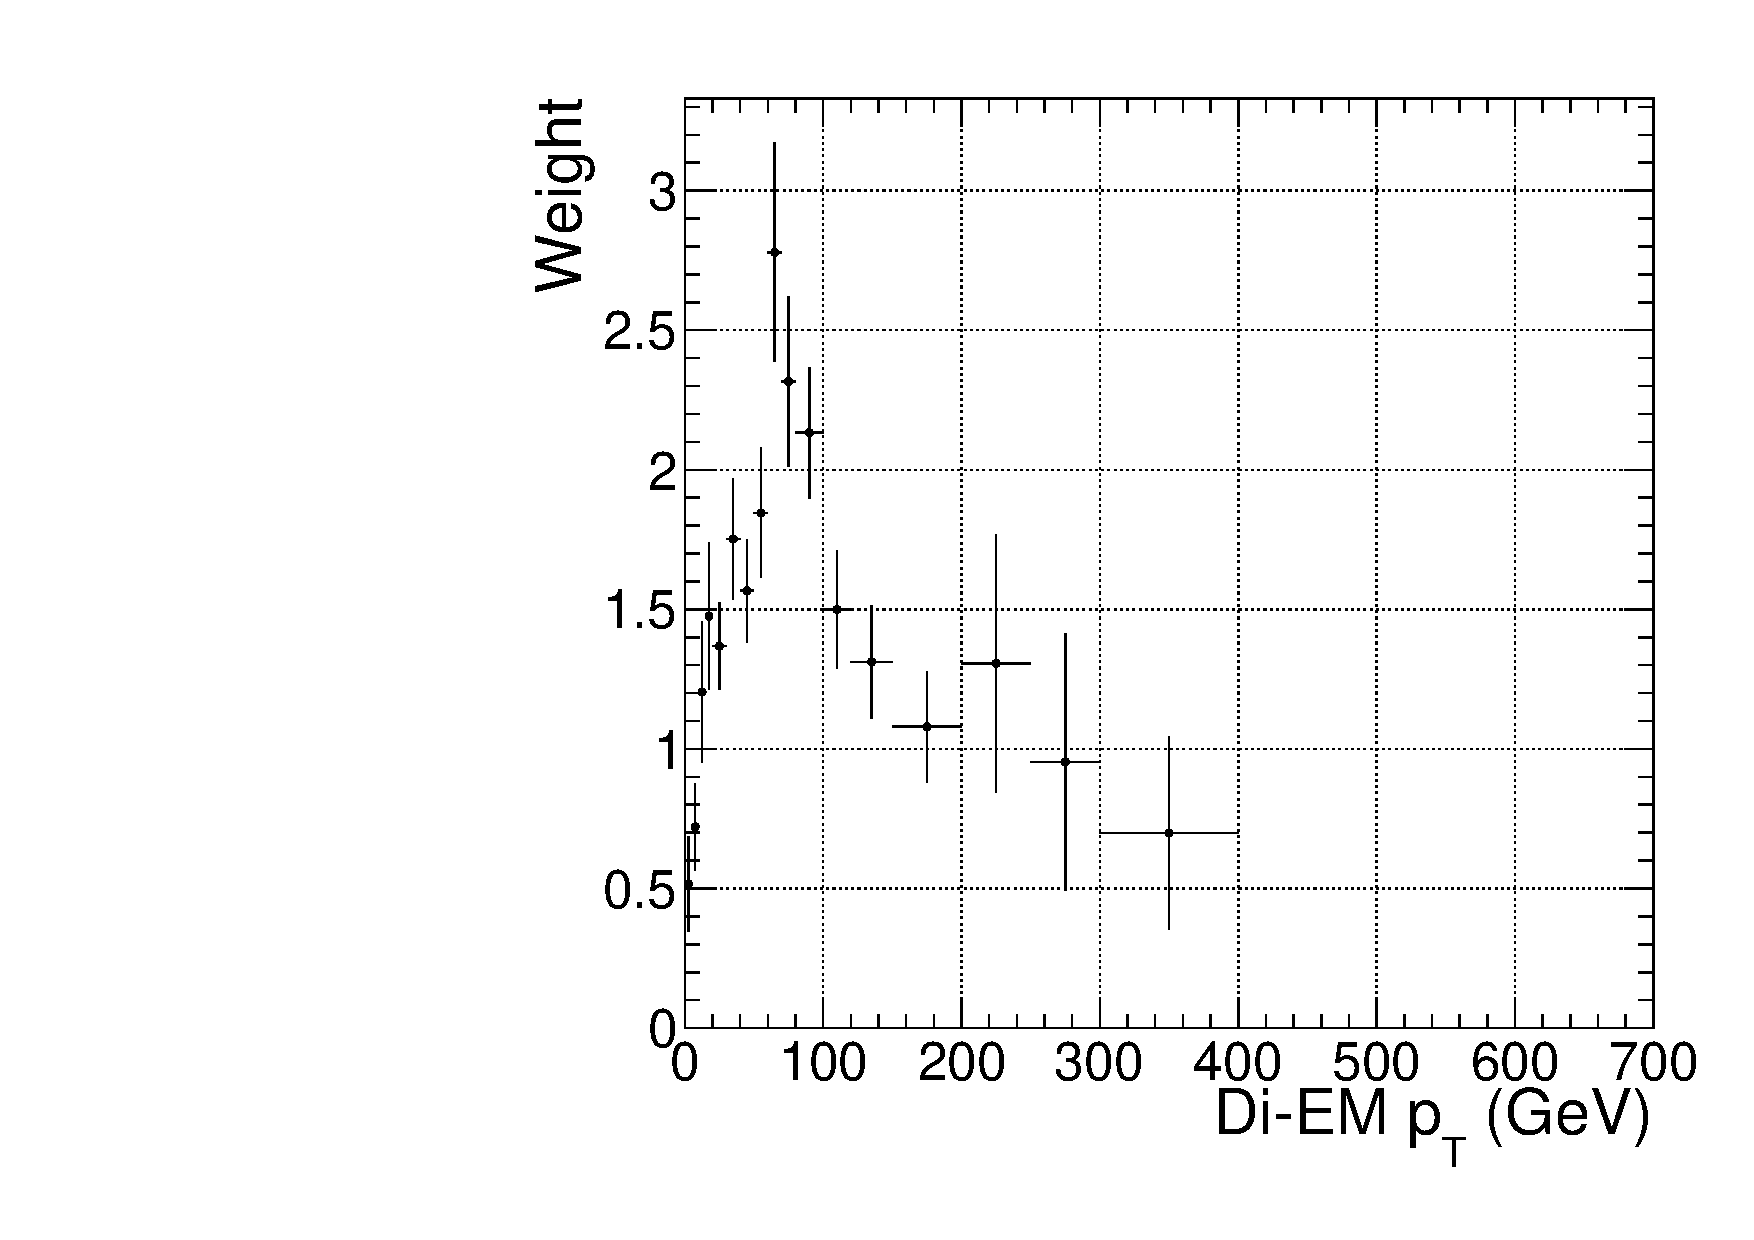
\includegraphics[scale=0.2]{eeHighSideband_2_jet_dijet_pT_weights}}	
	\caption{$ee$ sideband di-EM $p_{T}$ weights for events with 0, 1, or $\geq 2$ jets (as in Table~\ref{tab:jet_definition_for_Nj_reweighting}).  Errors are statistical only.}
	\label{fig:ee_sideband_dijet_pT_weights}
\end{figure}

\begin{figure}
	\centering
	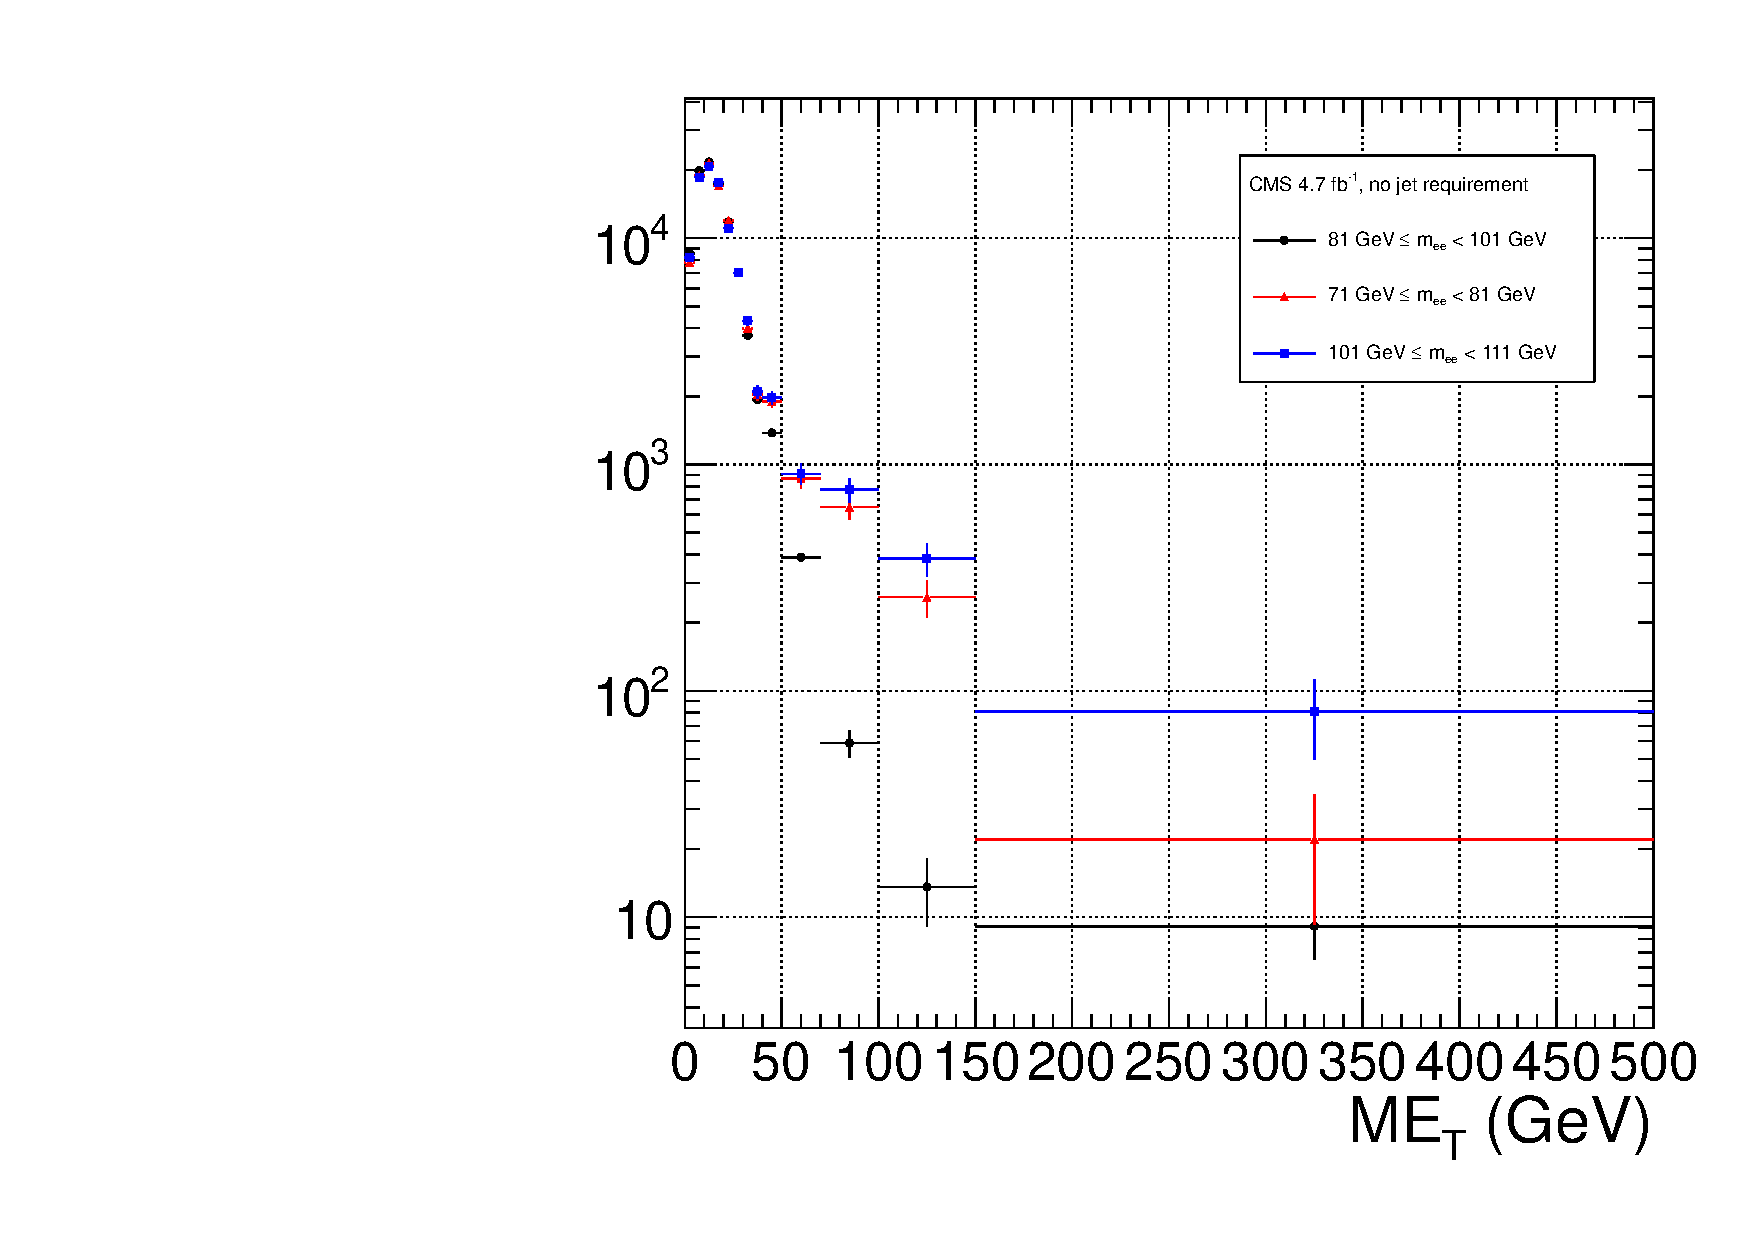
\includegraphics[scale=0.3]{all_ee_MET_spectra}
	\caption{\MET spectra of the $ee$ sample for 71 GeV $\leq m_{\mathrm{ee}} <$ 81 GeV (red triangles), 81 GeV $\leq m_{\mathrm{ee}} <$ 101 GeV (black circles), and 101 GeV $\leq m_{\mathrm{ee}} <$ 111 GeV (blue squares).  The two sideband distributions (red and blue) and the  $Z$ signal distribution (black) are normalized to the total number of $\gamma\gamma$ events.  Errors are statistical only.}
	\label{fig:all_ee_MET_spectra}
\end{figure}

The $ee$ (81 GeV $\leq m_{\mathrm{ee}} <$ 101 GeV), $\mathit{ff}$, and $\gamma\gamma$ di-EM $p_{T}$ spectra for events with 0, 1, or $\geq 2$ jets (as in Table~\ref{tab:jet_definition_for_Nj_reweighting}) are shown in Figure~\ref{fig:dijet_pT}.  Broad humps in the $\mathit{ff}$ and $\gamma\gamma$ spectra are due to kinematic $\Delta R$ and $p_{T}$ turn-ons that are suppressed in the $ee$ sample due to the invariant mass cut.  Figure~\ref{fig:dijet_pT_weights} shows the weights applied to the $ee$ (81 GeV $\leq m_{\mathrm{ee}} <$ 101 GeV) and $\mathit{ff}$ \MET spectra as a function of di-EM $p_{T}$ and number of jets per event.

%zoom out?
\begin{figure}
	\centering
	\subfloat[0 jets.]{\label{fig:0_jet_dijet_pT}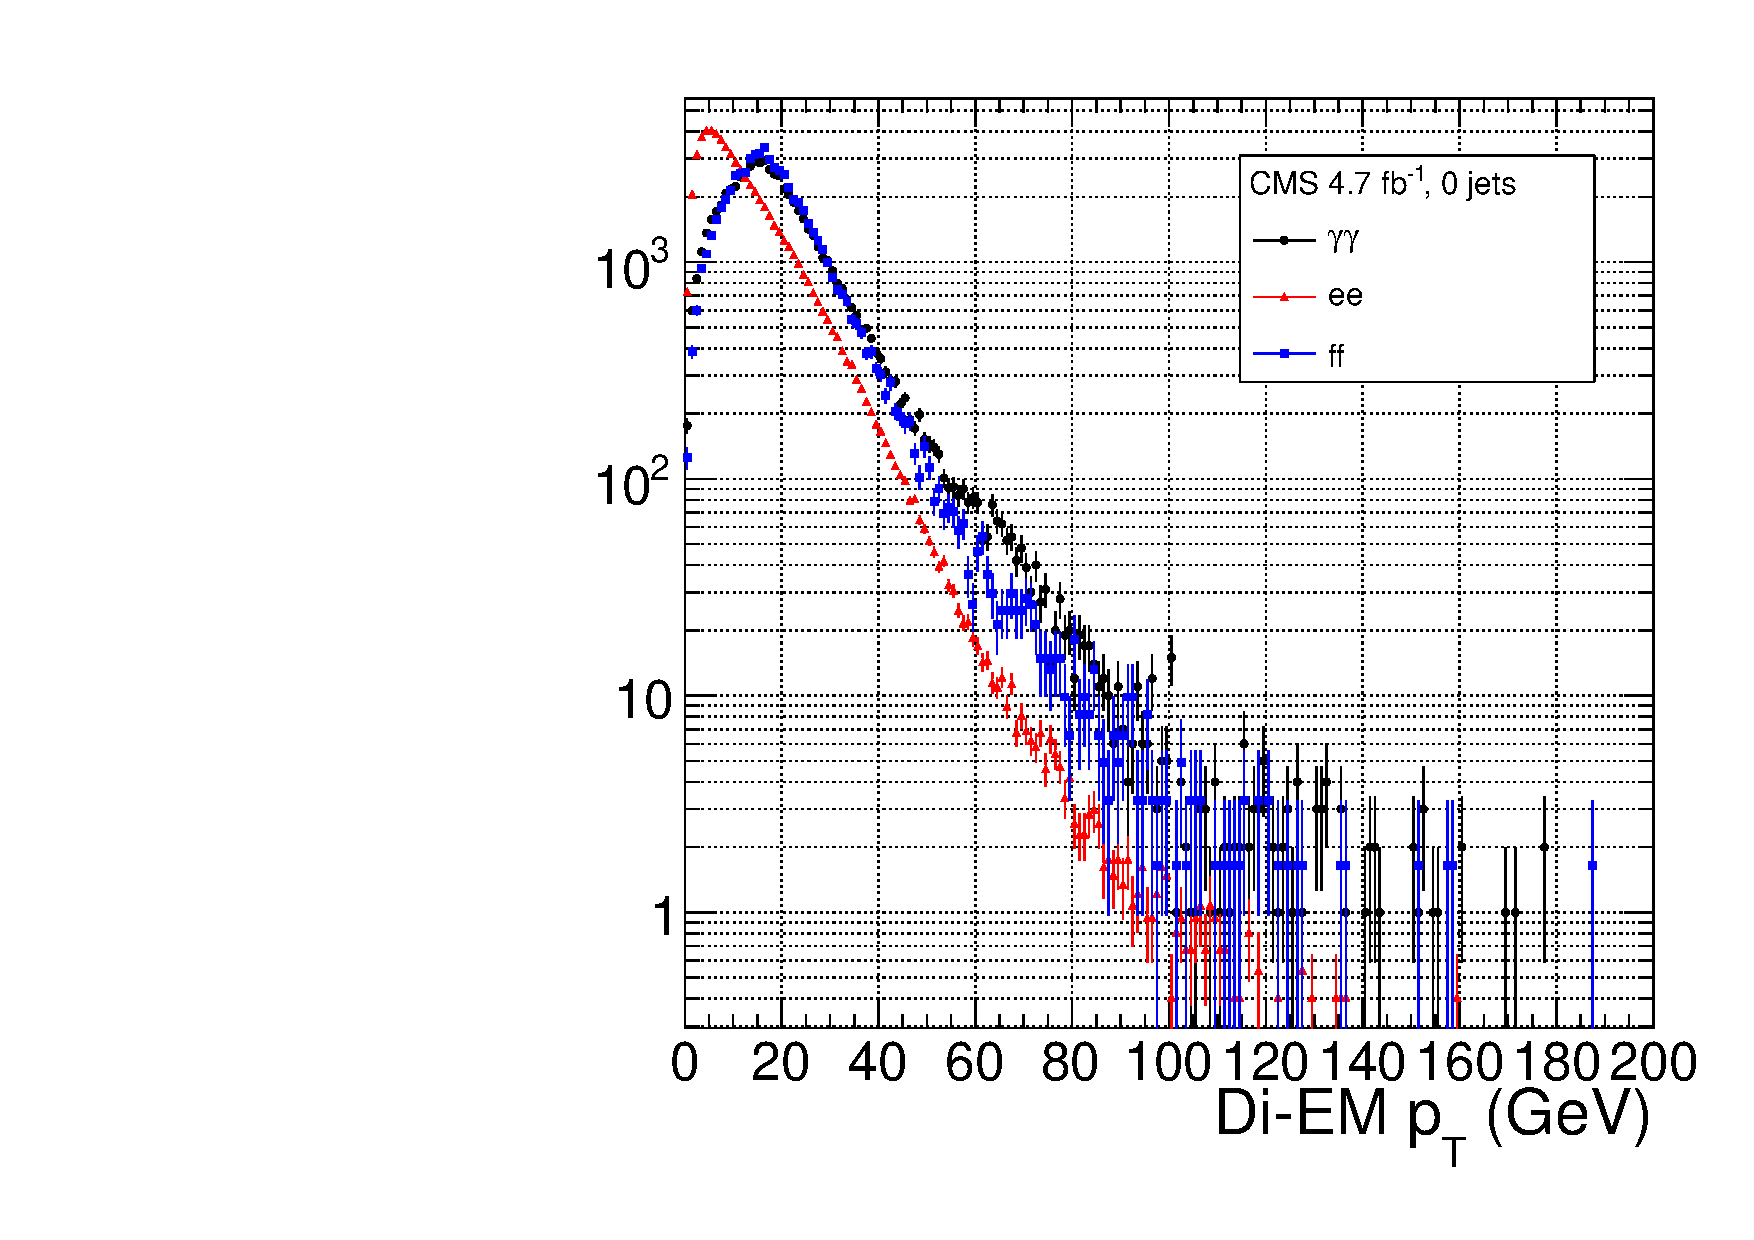
\includegraphics[scale=0.2]{0_jet_dijet_pT}}
	\hspace{1cm}
	\subfloat[1 jet.]{\label{fig:1_jet_dijet_pT}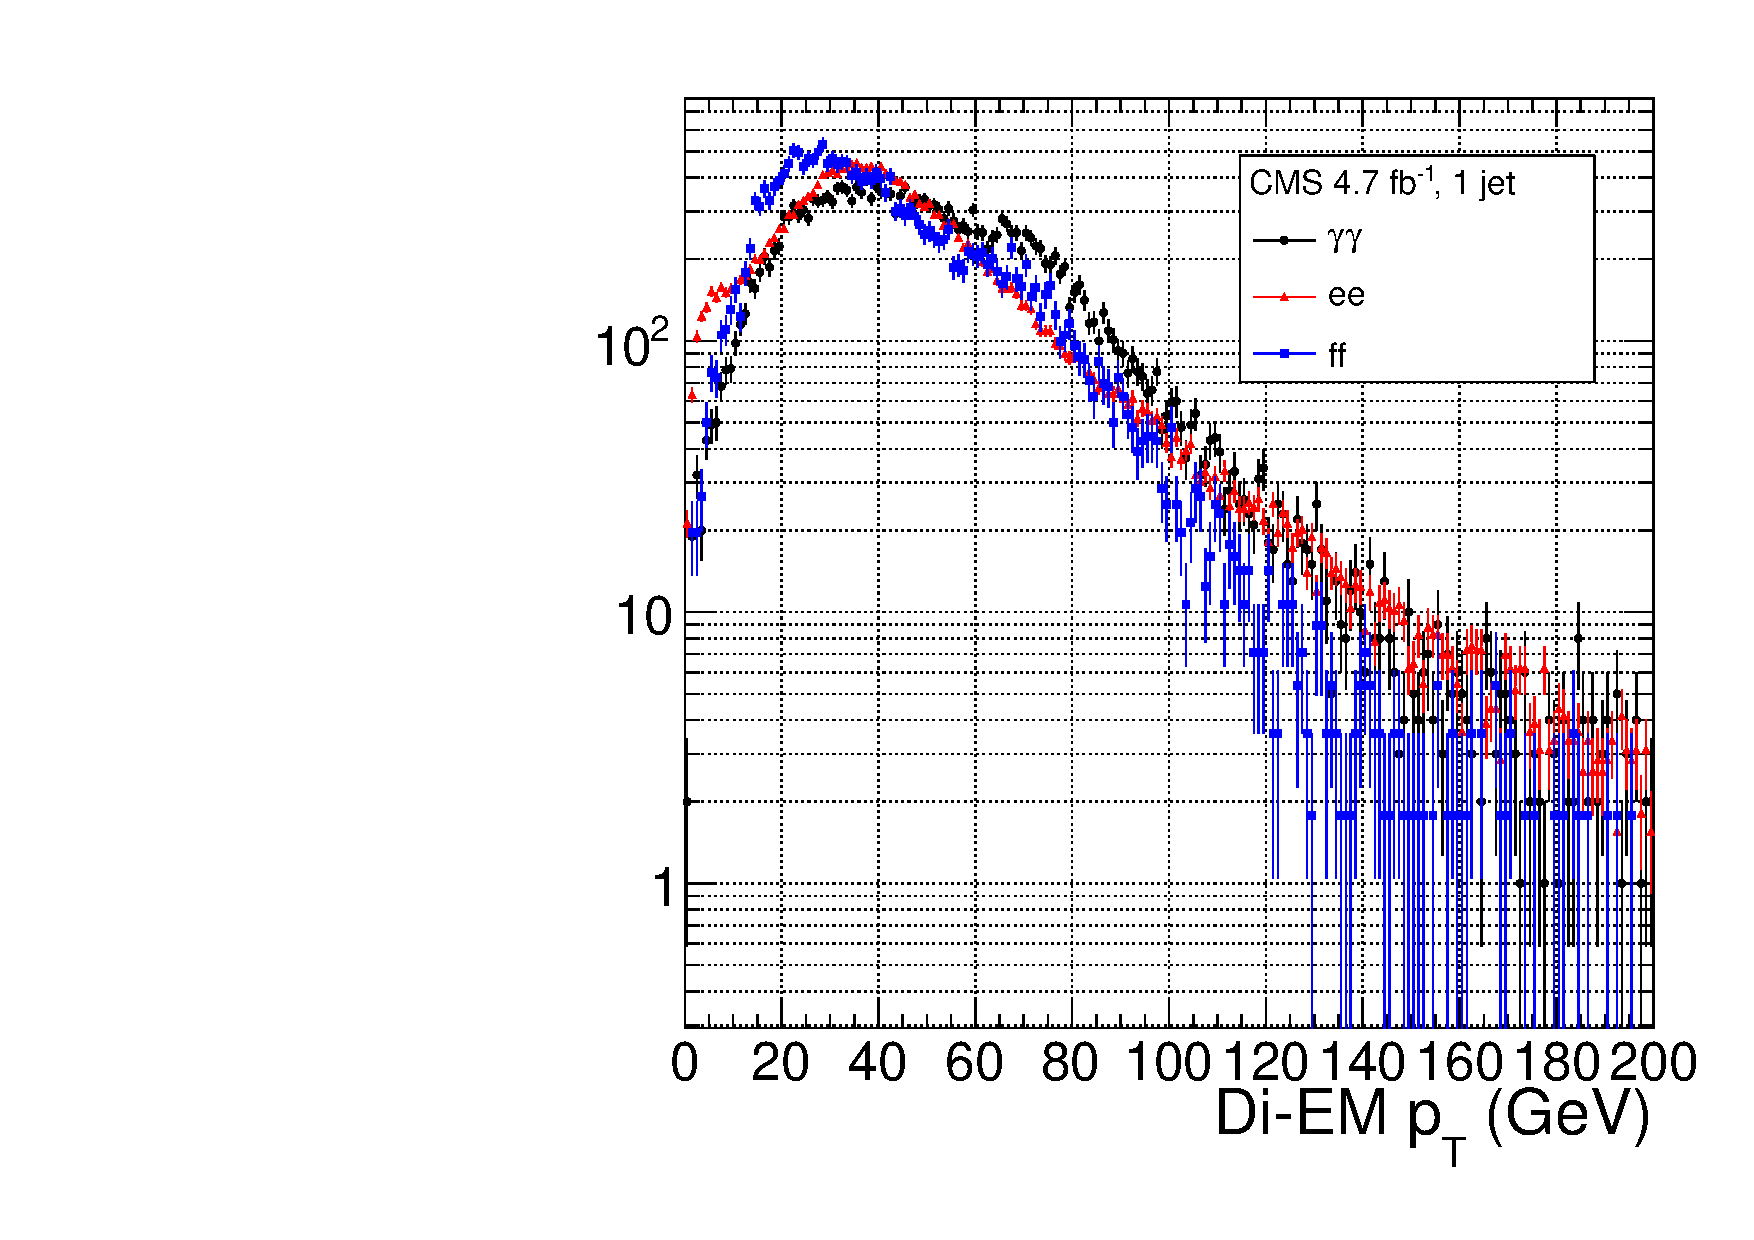
\includegraphics[scale=0.2]{1_jet_dijet_pT}}
	\hspace{1cm}
	\subfloat[$\geq$ 2 jets.]{\label{fig:2_jet_dijet_pT}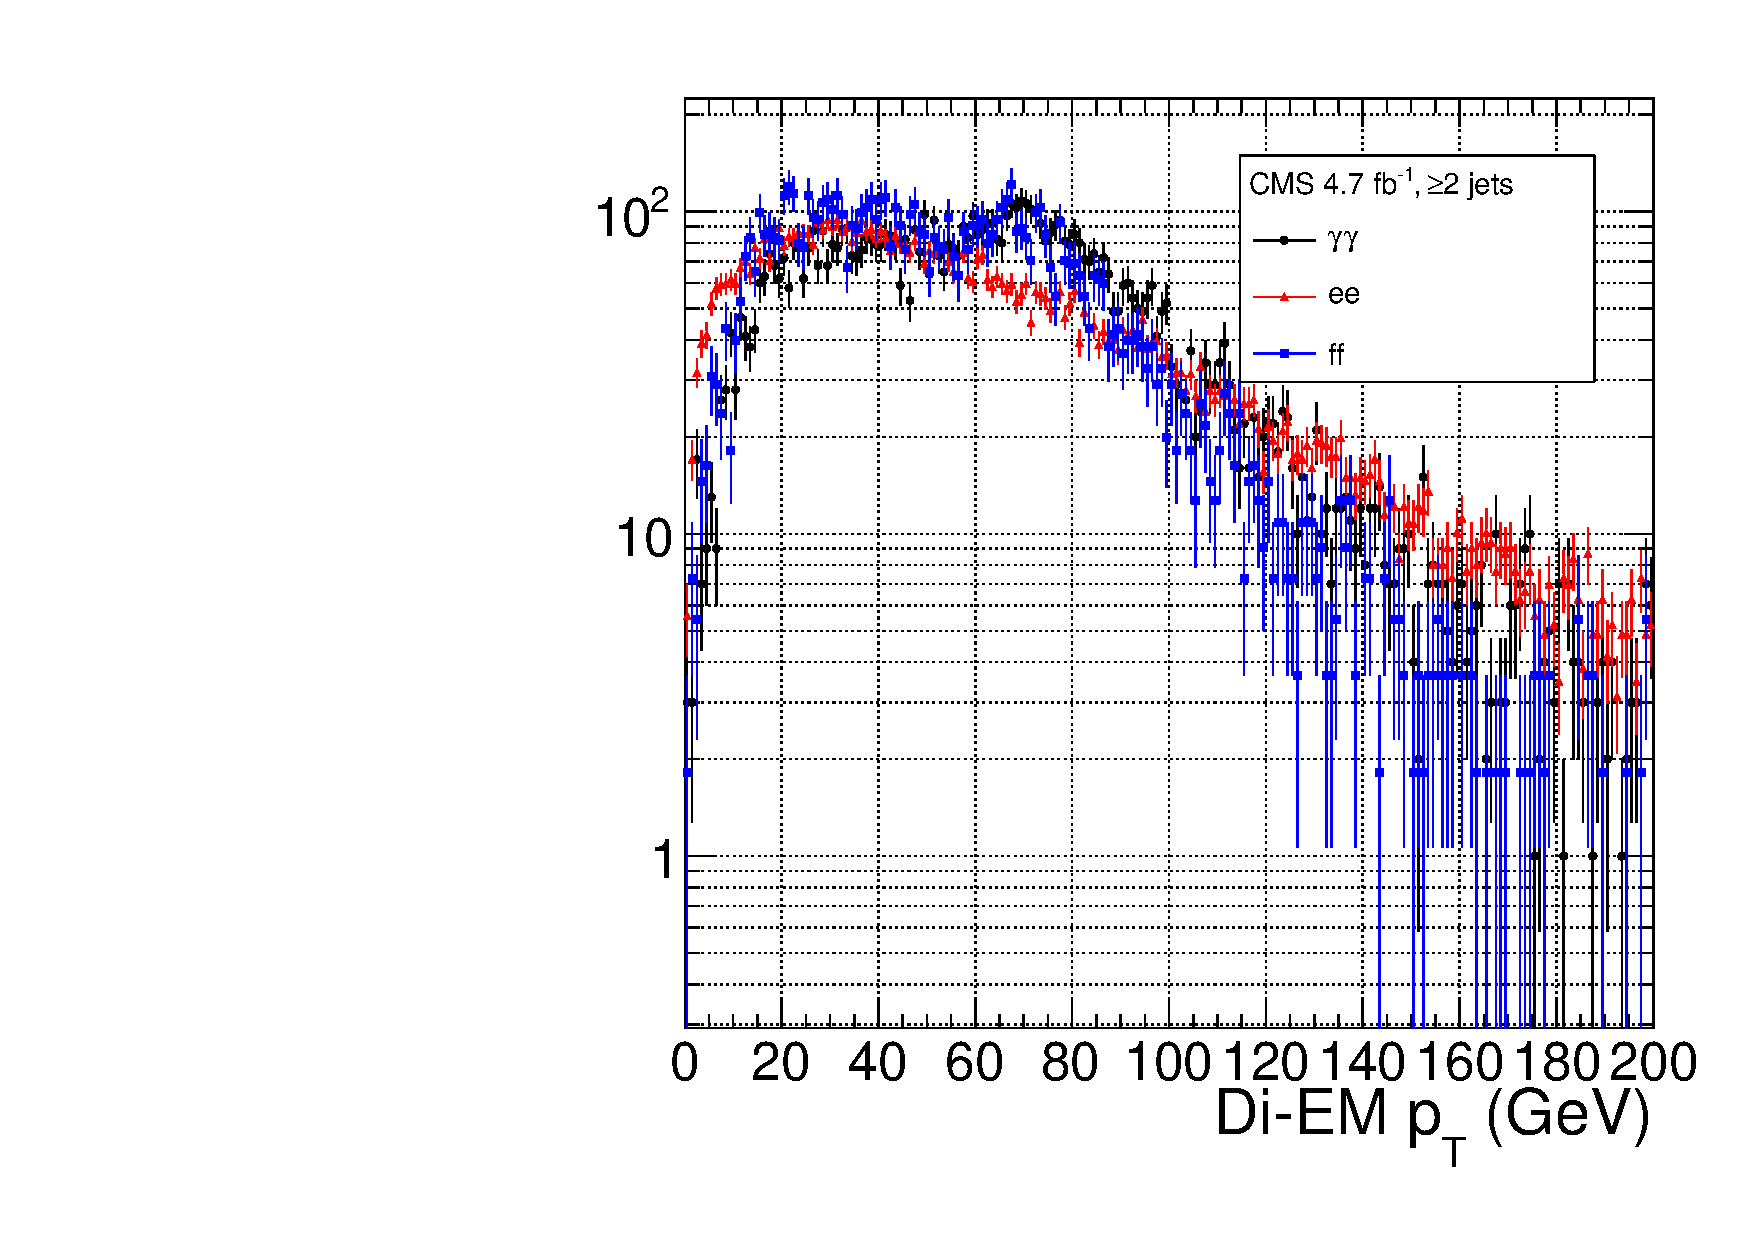
\includegraphics[scale=0.2]{2_jet_dijet_pT}}
	\caption{$ee$ (81 GeV $\leq m_{\mathrm{ee}} <$ 101 GeV) (red triangles), $\mathit{ff}$ (blue squares), and $\gamma\gamma$ (black circles) di-EM $p_{T}$ spectra for events with 0, 1, or $\geq 2$ jets (as in Table~\ref{tab:jet_definition_for_Nj_reweighting}).  Errors are statistical only.}
	\label{fig:dijet_pT}
\end{figure}

%zoom in?
\begin{figure}
	\centering
	\subfloat[$ee$, 0 jets.]{\label{fig:ee_0_jet_dijet_pT_weights}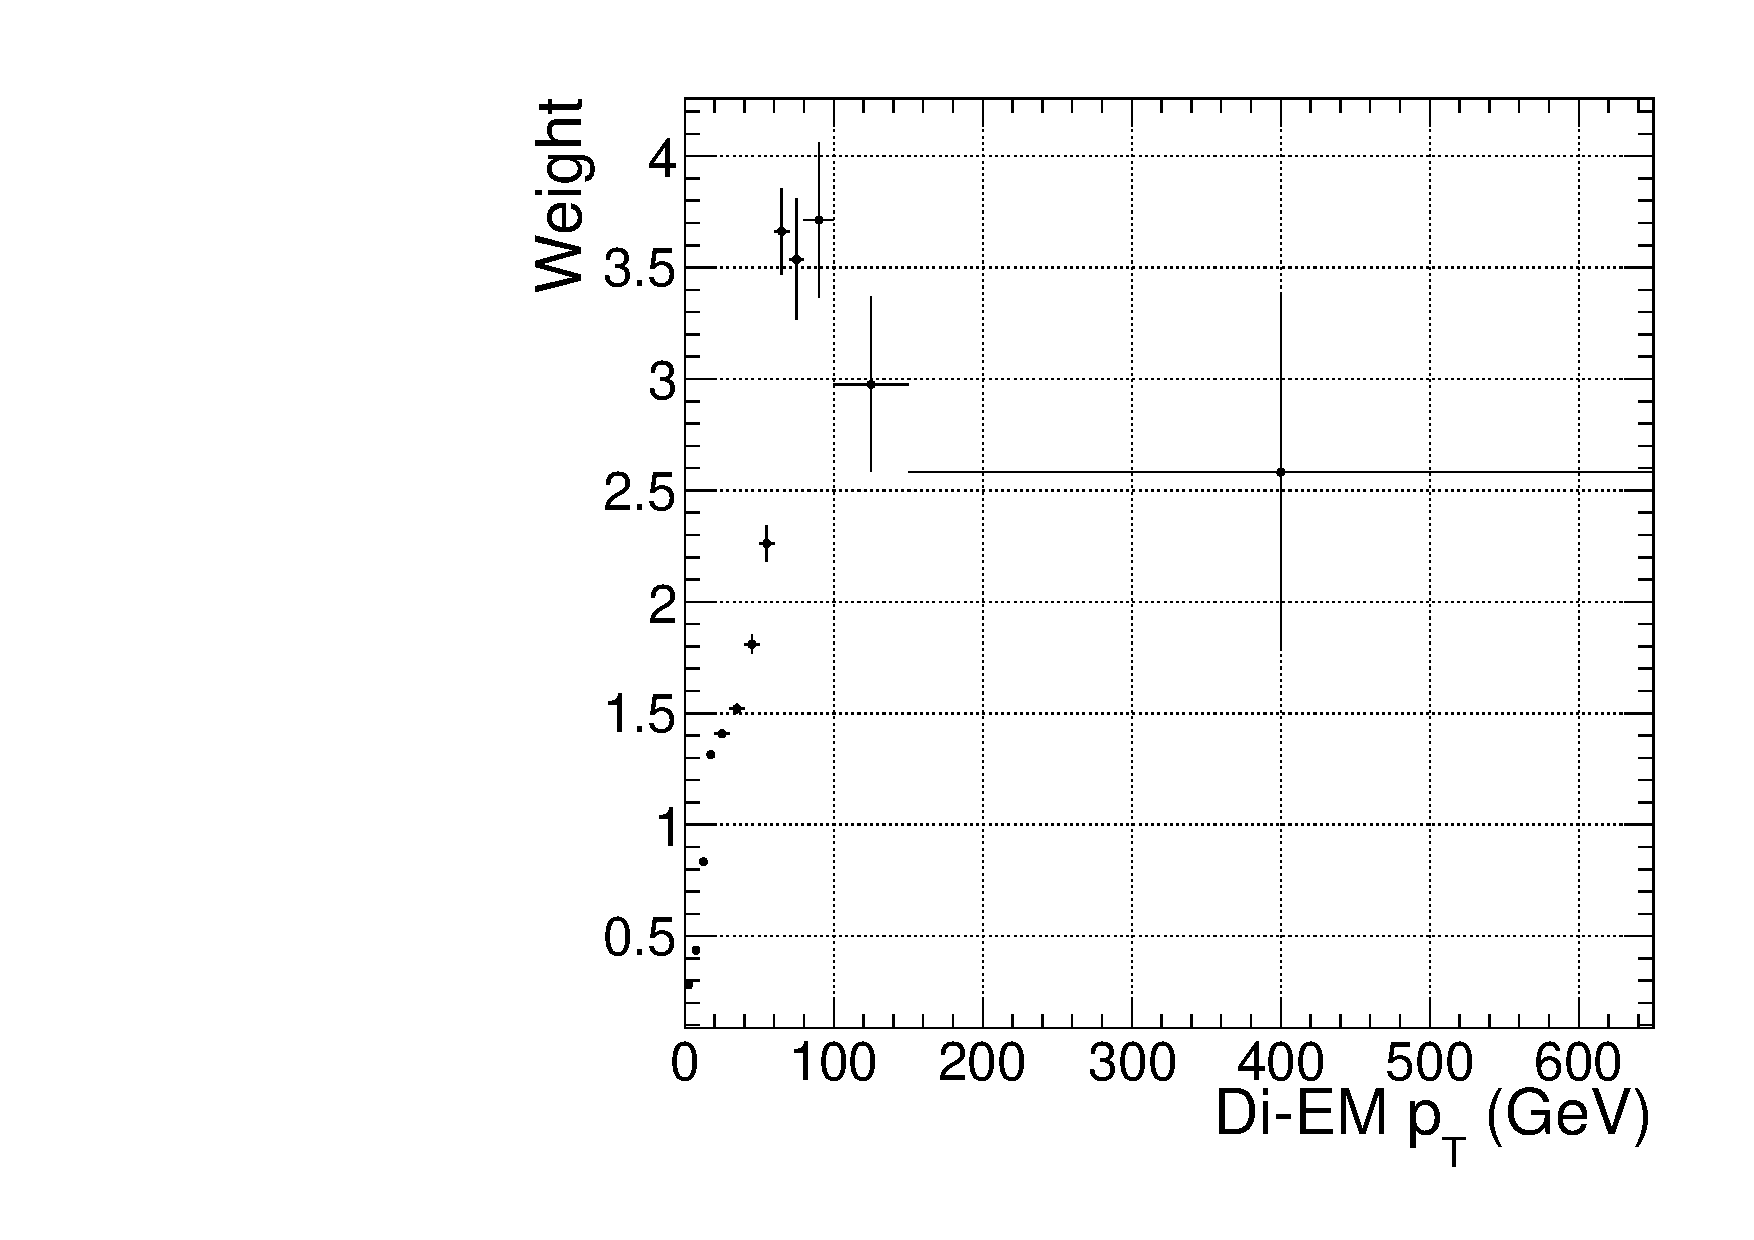
\includegraphics[scale=0.2]{ee_0_jet_dijet_pT_weights}}
	\hspace{1cm}
	\subfloat[$ee$, 1 jet.]{\label{fig:ee_1_jet_dijet_pT_weights}\includegraphics[scale=0.2]{ee_1_jet_dijet_pT_weights}}
	\hspace{1cm}
	\subfloat[$ee$, $\geq$ 2 jets.]{\label{fig:ee_2_jet_dijet_pT_weights}\includegraphics[scale=0.2]{ee_2_jet_dijet_pT_weights}}
	\\
	\subfloat[$\mathit{ff}$, 0 jets.]{\label{fig:ff_0_jet_dijet_pT_weights}\includegraphics[scale=0.2]{ff_0_jet_dijet_pT_weights}}
	\hspace{1cm}
	\subfloat[$\mathit{ff}$, 1 jet.]{\label{fig:ff_1_jet_dijet_pT_weights}\includegraphics[scale=0.2]{ff_1_jet_dijet_pT_weights}}
	\hspace{1cm}
	\subfloat[$\mathit{ff}$, $\geq$ 2 jets.]{\label{fig:ff_2_jet_dijet_pT_weights}\includegraphics[scale=0.2]{ff_2_jet_dijet_pT_weights}}
	\caption{$ee$ (81 GeV $\leq m_{\mathrm{ee}} <$ 101 GeV) and $\mathit{ff}$ di-EM $p_{T}$ weights for events with 0, 1, or $\geq 2$ jets (as in Table~\ref{tab:jet_definition_for_Nj_reweighting}).  Errors are statistical only.}
	\label{fig:dijet_pT_weights}
\end{figure}

\subsection{Normalization}
\label{sec:Normalization}

After reweighting, the \MET distributions of the QCD control samples are normalized to the \MET $< 20$ GeV region of the candidate $\gamma\gamma$ \MET spectrum, where signal contamination is low.  The normalization factor is ($N_{\gamma\gamma}^{\not\!\! E_{T} < 20 \mathrm{GeV}} - N_{e\gamma}^{\not\!\! E_{T} < 20 \mathrm{GeV}})/N_{\mathrm{control}}^{\not\!\! E_{T} < 20 \mathrm{GeV}}$, where $N_{e\gamma}^{\not\!\! E_{T} < 20 \mathrm{GeV}}$ is the expected number of electroweak background events with \MET $< 20$ GeV (discussed in Section~\ref{sec:Modeling the Electroweak Background}).

\section{Modeling the Electroweak Background}
\label{sec:Modeling the Electroweak Background}

$W\gamma$, $W$ + jet, and $t\bar{t}$ processes in which the $W$ decay electron is misidentified as a photon (due to a failure to properly associate a pixel seed to the electron candidate) can contribute significantly to the high-\MET tail of the $\gamma\gamma$ \MET spectrum.  To estimate this background, the $e\gamma$ sample, which is enriched in $W\rightarrow e\nu$ decays, is scaled by $f_{e\rightarrow\gamma}/(1 - f_{e\rightarrow\gamma})$, where $f_{e\rightarrow\gamma}$ is the rate at which electrons are misidentified as photons.  The derivation of this scaling factor comes from the two equations

\begin{eqnarray}
N_{e\gamma}^{W} &=& f_{e\rightarrow e}N_{W}\\
N_{\gamma\gamma}^{W} &=& (1 - f_{e\rightarrow e})N_{W}
\end{eqnarray}
%
where $N_{e\gamma}^{W}$ is the number of $W$ events in the $e\gamma$ sample in which the electron was correctly identified, $f_{e\rightarrow e}$ is the probability to correctly identify an electron, $N_{W}$ is the true number of triggered $W\rightarrow e\nu$ events, and $N_{\gamma\gamma}^{W}$ is the number of $W$ events in the $\gamma\gamma$ sample in which the electron was misidentified as a photon.  The contribution from $Z\rightarrow ee$ can be neglected (i.e. $f_{e\rightarrow\gamma}$ is small and the $Z$ contribution involves $f_{e\rightarrow\gamma}^{2}$, since both electrons have to be misidentified).  Since $f_{e\rightarrow e} = 1 - f_{e\rightarrow\gamma}$, solving for $N_{\gamma\gamma}^{W}$ gives

\begin{eqnarray}
N_{\gamma\gamma}^{W} = \frac{f_{e\rightarrow\gamma}}{1 - f_{e\rightarrow\gamma}}N_{e\gamma}^{W}
\end{eqnarray}

$f_{e\rightarrow\gamma}$ is measured by fitting the $Z$ peaks in the $ee$ and $e\gamma$ samples.  The number of $Z$ events fitted in the $ee$ and $e\gamma$ samples, respectively, is given by

\begin{eqnarray}
N_{ee}^{Z} &=& (1 - f_{e\rightarrow\gamma})^{2}N_{Z} \\
N_{e\gamma}^{Z} &=& 2f_{e\rightarrow\gamma}(1 - f_{e\rightarrow\gamma})N_{Z}
\end{eqnarray}
%
where $N_{Z}$ is the true number of triggered $Z\rightarrow ee$ events.  Solving for $f_{e\rightarrow\gamma}$ gives

\begin{eqnarray}
f_{e\rightarrow\gamma} = \frac{N_{e\gamma}^{Z}}{2N_{ee}^{Z} + N_{e\gamma}^{Z}}
\label{eq:feg}
\end{eqnarray}

A Crystal Ball function is used to model the $Z$ signal shape in both the $ee$ and $e\gamma$ samples, while an exponential convoluted with an error function (\verb+RooCMSShape+, see Sec.~\ref{sec:Tag_and_Probe_Method}) is used to model the background shape.  The fixed fit parameters are identical for the two samples, but the other parameters are allowed to float independently.  Table~\ref{tab:feg_fit_parameters} shows the values and ranges of the fixed and floating fit parameters, respectively.

\begin{table}[hcbp]
\caption{Parameter values for the signal and background PDFs for the $ee$ and $e\gamma$ samples.  When a bracketed range is given, the parameter is allowed to float within that range.  When a constant is given, the parameter is fixed to that constant.}
\centering
\begin{tabular}{|m{1.25cm}|m{1.25cm}|m{1.25cm}|m{1.25cm}|m{1.25cm}|m{1.25cm}|m{1.25cm}|m{1.25cm}|m{1.25cm}|}
\hline
& \multicolumn{4}{c|}{Crystal Ball fit parameters} & \multicolumn{4}{c|}{\texttt{RooCMSShape} fit parameters} \\
\hline
PDF & $\mu$ & $\sigma$ & $\alpha$ & n & $\mu$ & $\alpha$ & $\beta$ & $\gamma$ \\
\hline
$ee$ signal & [86.2, 96.2] & [1.0, 5.0] & 1.063 & 143.16 & N/A & N/A & N/A & N/A \\
\hline
$e\gamma$ signal & [86.2, 96.2] & [1.0, 5.0] & 1.063 & 143.16 & N/A & N/A & N/A & N/A \\
\hline
$ee$ background & N/A & N/A & N/A & N/A & 58 & 97.0 & 0.0922 & 0.191 \\
\hline
$e\gamma$ background & N/A & N/A & N/A & N/A & 56 & 72.02 & 0.098 & 0.0375 \\
\hline
\end{tabular}
\label{tab:feg_fit_parameters}
\end{table}

Fits to the $ee$ and $e\gamma$ invariant mass spectra are shown in Figure~\ref{fig:feg_fits}.  Figure~\ref{fig:feg_vs_pT_eta} indicates that the dependence of $f_{e\rightarrow\gamma}$ on the electron $p_{T}$ and $\eta$ is small.  (Note that all fit parameters are floating in the $p_{T}$-dependent fits.)  Therefore, a constant misidentification rate (derived from all $ee$ and $e\gamma$ events), rather than a $p_{T}$- and $\eta$-dependent misidentification rate, is used in the final electroweak background estimate, with the difference between the constant rate and the rate for electrons with $p_{T}$ between 25 and 40 GeV (the range in which the bulk of the trailing photons in the $\gamma\gamma$ sample lie) taken as a systematic error.

\begin{figure}
	\centering
	\subfloat[$ee$.]{\label{fig:mee_fit}\includegraphics[scale=0.3]{mee_fit}}
	\hspace{1cm}
	\subfloat[$e\gamma$.]{\label{fig:meg_fit}\includegraphics[scale=0.3]{meg_fit}}
	\caption{Fits to the $ee$ and $e\gamma$ invariant mass spectra using the Crystal Ball \texttt{RooCMSShape} function described in the text and in Table~\ref{tab:feg_fit_parameters}.  The total fit is shown in blue, while the background component is shown in red.}
	\label{fig:feg_fits}
\end{figure}

\begin{figure}
	\centering
	\subfloat[$f_{e\rightarrow\gamma}$ vs. electron $p_{T}$.  For the lowest $p_{T}$ bin, the fit to the $e\gamma$ spectrum does not converge well, so the $Z$ signal fraction is fixed to the value in Fig.~\ref{fig:meg_fit}.]{\label{fig:feg_vs_pT}\includegraphics[scale=0.3]{feg_vs_pT}}
	\hspace{1cm}
	\subfloat[$f_{e\rightarrow\gamma}$ vs. electron $\eta$.]{\label{fig:feg_vs_eta}\includegraphics[scale=0.3]{feg_vs_eta}}
	\caption{$f_{e\rightarrow\gamma}$ vs. electron $p_{T}$ and $\eta$.}
	\label{fig:feg_vs_pT_eta}
\end{figure}

Using the integrals of the $Z$ fits shown in Fig.~\ref{fig:feg_fits}, Eq.~\ref{eq:feg}, and the $p_{T}$ systematic discussed above, $f_{e\rightarrow\gamma}$ is calculated to be 0.014 $\pm$ 0.000(stat.) $\pm$ 0.004(syst.).  The scaled $e\gamma$ MET distribution is shown in Figure~\ref{fig:eg_MET}.

\begin{figure}
	\centering
	\includegraphics[scale=0.4]{eg_MET}
	\caption{\MET spectrum of the $e\gamma$ sample after scaling by $f_{e\rightarrow\gamma}$.  The total error on $f_{e\rightarrow\gamma}$ is propagated to the total error on the electroweak background estimate.}
	\label{fig:eg_MET}
\end{figure}

In the 36 $\mbox{pb}^{-1}$ version of this analysis \cite{CMS_GMSB_35pb-1}, it was shown that the $ee$ sample could accurately predict the QCD and real $Z$ contribution to the $e\gamma$ sample at low \MET, and that the expectation from $W\rightarrow e\nu$ MC accounted for the remaining $W$ contribution at high \MET.  A plot of the \MET distributions of the 2010 $e\gamma$ sample and the predicted components is shown in Figure~\ref{fig:35pb-1_eg_closure_test}.  This exercise helps to validate both the QCD and electroweak background prediction methods.

\begin{figure}
	\centering
	\includegraphics[scale=0.4]{35pb-1_eg_closure_test}
	\caption{\MET spectrum of the $e\gamma$ sample in 35 $\mbox{pb}^{-1}$ of 2010 LHC data scaled by the 2010 measured $f_{e\rightarrow\gamma}$ (black dots), QCD and real $Z$ predicted background from the 2010 $ee$ sample (solid orange line), MC $W$ + jet estimate (dash-dotted purple line), and MC $W\gamma$ estimate (dashed blue line).  The total $e\gamma$ prediction (red band) is the sum of the $ee$, $W$ + jet, and $W\gamma$ predictions.  Reprinted from Fig. 2 of ref. \cite{CMS_GMSB_35pb-1}.}
	\label{fig:35pb-1_eg_closure_test}
\end{figure}

\section{Errors on the Background Prediction}
\label{sec:Errors on the Background Prediction}

The statistical error on the final background estimate in a particular \MET bin comes from three sources: the number of control sample events collected in that bin, the statistical error on the weights applied to events in that bin, and the statistics of the normalization region.  In the case of the $ee$ control sample, there are contributions from the statistics of the $m_{\mathrm{ee}}$ sidebands as well.

In order to estimate the statistical error due to the reweighting procedure, 1000 toy sets of weights are generated.  Each set includes a weight for each (di-EM $p_{T}$, $N_{\mathrm{j}}$) bin, with the values picked from a Gaussian distribution with mean and standard deviation equal to the observed weight for that bin and its statistical error.  The effect of reweighting error is not correlated between \MET bins.  For each of the 1000 experiments, the control sample data are reweighted according to the generated weights, and the background estimates are calculated for each \MET bin.  Since the distribution of the toy background estimates follows a Gaussian distribution in each \MET bin, the RMS spread of the estimates is taken as the statistical error due to reweighting.  This procedure is carried out for the $\mathit{ff}$, $ee$, low sideband $ee$, and high sideband $ee$ samples.

The total statistical error on the background estimate per \MET bin is given by

\begin{eqnarray}
\sigma_{\mathrm{stat}}^{2} &=& \sigma_{\mathrm{stat,QCD}}^{2} + \sigma_{\mathrm{stat,EW}}^{2}
\label{eq:total_stat_error}
\end{eqnarray}
%
where $\sigma_{\mathrm{stat,QCD}}^{2}$ is the square of the total statistical error on the QCD prediction in the \MET bin

\begin{eqnarray}
\sigma_{\mathrm{stat,QCD}}^{2} &=& \sigma_{\mathrm{stat,}s}^{2} + \sigma_{\mathrm{Poisson,QCD}}^{2} + \sigma_{\mathrm{reweight,}s}^{2} + \sigma_{\mathrm{reweight,QCD}}^{2}
\label{eq:QCD_stat_error}
\end{eqnarray}
%
and $\sigma_{\mathrm{stat,EW}}$ is the Poisson error on the number of $e\gamma$ events in the \MET bin (= $\sqrt{N_{e\gamma}}$, where $N_{e\gamma}$ is the prediction in the \MET bin after scaling by $f_{e\rightarrow\gamma}$).  The contributions to $\sigma_{\mathrm{stat,QCD}}^{2}$ are discussed below.

\begin{itemize}

\item $\sigma_{\mathrm{stat,}s}^{2}$ is the statistical error contributed by the normalization factor $s$ (i.e. from Poisson error in the normalization region \MET $<$ 20 GeV):

\begin{eqnarray}
\sigma_{\mathrm{stat,}s}^{2} &=& \frac{N_{\mathrm{control}}^{2}}{(N_{\gamma\gamma}^{\mathrm{norm}} - N_{e\gamma}^{\mathrm{norm}})^{2}}(\left[\sigma_{\mathrm{Poisson,}\gamma\gamma}^{\mathrm{norm}}\right]^{2} + \left[\sigma_{\mathrm{Poisson,}e\gamma}^{\mathrm{norm}}\right]^{2}) + \nonumber \\
&&\frac{N_{\mathrm{control}}^{2}}{(N_{\mathrm{control}}^{\mathrm{norm}})^{2}}(\sigma_{\mathrm{Poisson,control}}^{\mathrm{norm}})^{2}
\label{eq:norm_stat_error}
\end{eqnarray}
%
where $N_{\mathrm{control}}$ is the number of reweighted, normalized events in the \MET bin, $N_{\gamma\gamma}^{\mathrm{norm}}$ is the number of $\gamma\gamma$ events in the normalization region, $N_{e\gamma}^{\mathrm{norm}}$ is the number of $e\gamma$ events in the normalization region (after scaling by $f_{e\rightarrow\gamma}$), $\sigma_{\mathrm{Poisson,}\gamma\gamma}^{\mathrm{norm}}$ is the Poisson error on the number of $\gamma\gamma$ events in the normalization region (= $\sqrt{N_{\gamma\gamma}^{\mathrm{norm}}}$), $\sigma_{\mathrm{Poisson,}e\gamma}^{\mathrm{norm}}$ is the Poisson error on the number of $e\gamma$ events in the normalization region (= $\sqrt{N_{e\gamma}^{\mathrm{norm}}}$), $N_{\mathrm{control}}^{\mathrm{norm}}$ is the number of QCD control ($ee$ or $\mathit{ff}$) events in the normalization region, and $\sigma_{\mathrm{Poisson,control}}^{\mathrm{norm}}$ is the Poisson error on the number of QCD control ($ee$ or $\mathit{ff}$) events in the normalization region (= $\sqrt{\sum_{i = 1}^{N_{\mathrm{control}}^{\mathrm{norm}}}w_{i}^{2}}$, where $w_{i}$ is the di-EM $p_{T}$ weight applied to event $i$).  For the $ee$ control region, $N_{\mathrm{control}}$ and $N_{\mathrm{control,norm}}$ are sideband subtracted, and $\sigma_{\mathrm{Poisson,control}}^{\mathrm{norm}}$ includes the Poisson error on the number of sideband events.

\item $\sigma_{\mathrm{Poisson,QCD}}$ is the Poisson error due to the number of QCD control ($ee$ or $\mathit{ff}$) events in the \MET bin, equal to $\sqrt{\sum_{i = 1}^{N_{\mathrm{control}}}w_{i}^{2}}$, where $w_{i}$ is the di-EM $p_{T}$ weight applied to event $i$.  For the $ee$ control region, $\sigma_{\mathrm{Poisson,QCD}}$ includes the Poisson error on the number of subtracted  sideband events.

\item $\sigma_{\mathrm{reweight,}s}$ is the error contributed by the control sample reweighting in the normalization region (= $\frac{N_{\mathrm{control}}^{2}}{(N_{\mathrm{control}}^{\mathrm{norm}})^{2}}\sigma_{\mathrm{reweight,control}}^{\mathrm{norm}}$).  $\sigma_{\mathrm{reweight,control}}^{\mathrm{norm}}$ is the quadrature sum of the RMS of the 1000 toy reweighting experiments for each \MET bin in the normalization region.  For the $ee$ control sample, it also includes (in quadrature) the RMS of the toys in the sideband samples.

\item $\sigma_{\mathrm{reweight,QCD}}$ is the error contributed by the control sample reweighting in the \MET bin (= $s\sigma_{\mathrm{reweight,control}}$).  $\sigma_{\mathrm{reweight,control}}$ is the RMS of the 1000 toy reweighting experiments for the \MET bin.  For the $ee$ control sample, it also includes (in quadrature) the RMS of the toys in the sideband samples.

\end{itemize}

The dominant source of systematic error on the background estimate is the slight difference in hadronic activity between the $ee$, $\mathit{ff}$, and $\gamma\gamma$ samples.  This results in a small bias ($\sim$1 GeV) of the $ee$ \MET distribution towards lower values with respect to the $\mathit{ff}$ and $\gamma\gamma$ samples, as shown in Figure~\ref{fig:avg_MET_vs_di-EM_pT}.  Therefore, the $\mathit{ff}$ sample is used as the primary QCD background estimator, and the difference between the $ee$ and $\mathit{ff}$ predictions is assigned as an error on the knowledge of the hadronic activity.  For \MET $>$ 100 GeV, this error amounts to 43\% of the total QCD + electroweak background estimate.

\begin{figure}
	\centering
	\includegraphics[scale=0.4]{avg_MET_vs_di-EM_pT}
	\caption{Average \MET vs. di-EM $p_{T}$ for the $\mathit{ff}$ (blue), $ee$ (red), and $\gamma\gamma$ (black) samples.}
	\label{fig:avg_MET_vs_di-EM_pT}
\end{figure}

The second largest source of systematic error comes from the $p_{T}$ dependence of the $e\rightarrow\gamma$ misidentification rate (see~\ref{sec:Modeling the Electroweak Background}).  For \MET $>$ 100 GeV, the expected electroweak background is 3.4 $\pm$ 1.0 events, so this error amounts to 4.8\% of the total QCD + electroweak background estimate.

The assumption of a constant $t\bar{t}$ and $W$ + jets background shape under the $Z$ peak in the $ee$ sample induces a systematic error on the $ee$ sideband-subtracted background prediction.  To assess the magnitude of this error, the sideband subtraction (see Sec.~\ref{sec:Reweighting}) is performed once using only the prediction from the high sideband, and once using only the prediction from the low sideband.  In each of these cases, the prediction is weighted by a factor of two, to account for the fact that the sideband regions are only half as wide (10 GeV) as the signal region (20 GeV).  The maximum variation from the nominal $ee$ estimate is taken as the error, which amounts to 11\% for \MET $>$ 100 GeV.  \MET distributions using the nominal $ee$ sideband subtraction, the low-sideband-only subtraction, and the high-sideband-only subtraction are shown in Figure~\ref{fig:mee_bkg_shape_error}.

\marginpar{\textcolor{blue}{Added this paragraph}}Finally, the few percent error on the jet energy correction factors introduces an error on the final background estimate through (a) the use of the PF $p_{T}$ to measure the di-EM $p_{T}$, (b) the counting of jets passing a 30 GeV $p_{T}$ threshold for placement of the event in an $N_{\mathrm{j}}$ bin for reweighting, and (c) the counting of jets above threshold for the $\geq1$-jet version of the selection.  To estimate this error, 100 pseudo-experiments are generated with identical properties as the true data sample, except with corrected jet energies (in all events) all shifted by an amount $r\sigma(p_{T}, \eta)$.  $r$ is a random number drawn from a Gaussian distribution with mean 0 and width 1, and $\sigma(p_{T}, \eta)$ is the uncertainty on the jet energy correction factor (which, like the correction factor itself, is a function of $p_{T}$ and $\eta$).  The same factor $r$ is applied to all jets in all events in the pseudo-experiment because the jet energy correction errors are correlated from jet to jet (they result from e.g. uncertainties in MC simulation or uncertainties in ECAL energy scale \cite{CMS_JES_paper}).  The standard error of the mean of the 100 resulting background estimates in each relevant \MET bin is taken as the error.  The error in each \MET bin is assumed to be uncorrelated.  This process is repeated for both the inclusive and $\geq1$-jet selections.  For \MET $\geq$ 100 GeV, the jet energy correction uncertainty is 1.5\%(2.2\%) of the total background for the inclusive($\geq$1-jet) selection.

\begin{figure}
	\centering
	\includegraphics[scale=0.4]{mee_bkg_shape_error}
	\caption{$ee$ \MET distributions using the nominal sideband subtraction (black circles), low sideband only (red squares), and high sideband only (blue triangles).  The bottom plot shows the ratio of the low sideband distribution to the nominal (red squares) and the ratio of the high sideband distribution to the nominal (blue triangles).}
	\label{fig:mee_bkg_shape_error}
\end{figure}

The uncertainty in how to define the (di-EM $p_{T}$, $N_{\mathrm{j}}$) bins, especially at high di-EM $p_{T}$ where the statistics are low, is covered by the 1000-toys procedure as long as the bins are not too coarse.  This is shown in Figure~\ref{fig:di-EM_pT_bin_size_comparison}.  If the bins are too coarse, the details of the shape of the di-EM $p_{T}$ spectra are lost, and the reweighting has a smaller effect.

\begin{figure}
	\centering
	\subfloat[$ee$.]{\label{fig:ee_di-EM_pT_bin_size_comparison}\includegraphics[scale=0.3]{ee_di-EM_pT_bin_size_comparison}}
	\hspace{1cm}
	\subfloat[$\mathit{ff}$.]{\label{fig:ff_di-EM_pT_bin_size_comparison}\includegraphics[scale=0.3]{ff_di-EM_pT_bin_size_comparison}}
	\caption{Comparison of \MET distributions for five different di-EM $p_{T}$ bin definitions: uniform bins of width 10 GeV (red diamonds); uniform bins of width 50 GeV (blue downward-pointing triangles); bins with lower edges \{0.0, 5.0, 10.0, 15.0, 20.0, 30.0, 40.0, 50.0, 60.0, 70.0, 80.0, 100.0, 750.0\} GeV for 0-jet events and \{0.0, 5.0, 10.0, 15.0, 20.0, 30.0, 40.0, 50.0, 60.0, 70.0, 80.0, 100.0, 120.0, 150.0, 200.0, 700.0\} GeV for $\geq$1-jet events (magenta upward-pointing triangles), i.e. a single wide bin at high di-EM $p_{T}$; bins with lower edges \{0.0, 5.0, 10.0, 15.0, 20.0, 30.0, 40.0, 50.0, 60.0, 70.0, 80.0, 100.0, 150.0\} GeV for 0-jet events and \{0.0, 5.0, 10.0, 15.0, 20.0, 30.0, 40.0, 50.0, 60.0, 70.0, 80.0, 100.0, 120.0, 150.0, 200.0\} GeV for $\geq$1-jet events (green squares), i.e. the bins used in ref. \cite{CMS_GMSB_5fb-1}; and the nominal bin definitions shown in Fig.~\ref{fig:dijet_pT_weights} (black circles).}
	\label{fig:di-EM_pT_bin_size_comparison}
\end{figure}

The use of uncorrected instead of corrected PF \MET (see Sec.~\ref{sec:MET}) makes no difference in the agreement of the background predictions and the search sample in a control region at low \MET, as shown in Figure~\ref{fig:Type-I_MET_corrections_vs_uncorrected_MET_zoom}.  Since the control samples are derived from the same data as the search sample, any biases in the \MET reconstruction due to jet energy scale are present equally in both samples.

\begin{figure}
	\centering
	\subfloat[Ratio of $\gamma\gamma$ to $ee$ \MET distributions.]{\label{fig:gg_over_ee_Type-I_MET_corrections_vs_uncorrected_MET_zoom}\includegraphics[scale=0.3]{gg_over_ee_Type-I_MET_corrections_vs_uncorrected_MET_zoom}}
	\hspace{1cm}
	\subfloat[Ratio of $\gamma\gamma$ to $\mathit{ff}$ \MET distributions.]{\label{fig:gg_over_ff_Type-I_MET_corrections_vs_uncorrected_MET_zoom}\includegraphics[scale=0.3]{gg_over_ff_Type-I_MET_corrections_vs_uncorrected_MET_zoom}}
	\hspace{1cm}
	\subfloat[Ratio of $ee$ to $\mathit{ff}$ \MET distributions.]{\label{fig:ee_over_ff_Type-I_MET_corrections_vs_uncorrected_MET_zoom}\includegraphics[scale=0.3]{ee_over_ff_Type-I_MET_corrections_vs_uncorrected_MET_zoom}}
	\caption{Agreement between $\gamma\gamma$, $ee$, and $\mathit{ff}$ samples for uncorrected (red triangles) and corrected (blue squares) \MET.}
	\label{fig:Type-I_MET_corrections_vs_uncorrected_MET_zoom}
\end{figure}

Tables~\ref{tab:ee_background_prediction_errors} and~\ref{tab:ff_background_prediction_errors} list all the errors on the $ee$ and $\mathit{ff}$ QCD background predictions, respectively, for the \MET bins used in the search.  Table~\ref{tab:eg_background_prediction_errors} lists the errors on the electroweak background prediction.  Finally, Table~\ref{tab:total_background_prediction_errors} shows the errors on the total QCD + electroweak background prediction, broken down by origin (statistical or systematic) and QCD background estimation sample ($ee$ or $\mathit{ff}$).  In the final result, only the $\mathit{ff}$ QCD estimate is used.

\begin{table}[hcbp]
\caption{Errors on the $ee$ QCD background prediction as a fraction of the $ee$ prediction.}
\centering
\begin{tabular}{|p{5cm}|c|c|c|c|c|}
\hline
\multicolumn{1}{|c|}{\multirow{2}{*}{Source of error}} & \multicolumn{5}{c|}{Fractional uncertainty (\%)} \\
\cline{2-6}
& [50, 60) & [60, 70) & [70, 80) & [80, 100) & $\geq$100 \\
\hline
\hline
Total & 3.9 & 8.1 & 16 & 25 & 25 \\
\hline
\hspace{0.5cm}Statistics & 3.6 & 7.8 & 16 & 24 & 22 \\
\hline
\hspace{1cm}No. events & 3.6 & 7.7 & 15 & 24 & 20 \\
\hspace{1.5cm}In norm. region & 0.43 & 0.44 & 0.46 & 0.55 & 0.51 \\
\hspace{1.5cm}In this \MET bin & 3.5 & 7.7 & 15 & 24 & 20 \\
\hline
\hspace{1cm}Reweighting & 0.73 & 1.2 & 3.5 & 4.3 & 7.7 \\
\hspace{1.5cm}In norm. region & 0.19 & 0.19 & 0.2 & 0.24 & 0.23 \\
\hspace{1.5cm}In this \MET bin & 0.71 & 1.2 & 3.5 & 4.3 & 7.7 \\
\hline
\hspace{0.5cm}Systematics & 2.6 & 4.4 & 1.2 & 7.5 & 14 \\
\hline
\hspace{1cm}$f_{e\rightarrow\gamma}$ (in norm. region) & 0.0012 & 0.0012 & 0.0013 & 0.0015 & 0.0014 \\
\hspace{1cm}$m_{ee}$ background shape & 1.4 & 2 & 0.72 & 5.5 & 12 \\
\hspace{1cm}Jet energy scale & 2.2 & 3.9 & 0.96 & 5.1 & 6.9 \\
\hline
%w/o JES systematic
%Total & 3.9 & 8.1 & 16 & 25 & 25 \\
%\hline
%\hspace{0.5cm}Statistics & 3.6 & 7.8 & 16 & 24 & 22 \\
%\hline
%\hspace{1cm}No. events & 3.6 & 7.7 & 15 & 24 & 20 \\
%\hspace{1.5cm}In norm. region & 0.43 & 0.44 & 0.46 & 0.55 & 0.51 \\
%\hspace{1.5cm}In this \MET bin & 3.5 & 7.7 & 15 & 24 & 20 \\
%\hline
%\hspace{1cm}Reweighting & 0.73 & 1.2 & 3.5 & 4.3 & 7.7 \\
%\hspace{1.5cm}In norm. region & 0.19 & 0.19 & 0.2 & 0.24 & 0.23 \\
%\hspace{1.5cm}In this \MET bin & 0.71 & 1.2 & 3.5 & 4.3 & 7.7 \\
%\hline
%\hspace{0.5cm}Systematics & 1.4 & 2 & 0.72 & 5.5 & 12 \\
%\hline
%\hspace{1cm}$f_{e\rightarrow\gamma}$ (in norm. region) & 0.0012 & 0.0012 & 0.0013 & 0.0015 & 0.0014 \\
%\hspace{1cm}$m_{ee}$ background shape & 1.4 & 2 & 0.72 & 5.5 & 12 \\
%\hline
\end{tabular}
\label{tab:ee_background_prediction_errors}
\end{table}

\begin{table}[hcbp]
\caption{Errors on the $\mathit{ff}$ QCD background prediction as a fraction of the $\mathit{ff}$ prediction.}
\centering
\begin{tabular}{|p{5cm}|c|c|c|c|c|}
\hline
\multicolumn{1}{|c|}{\multirow{2}{*}{Source of error}} & \multicolumn{5}{c|}{Fractional uncertainty (\%)} \\
\cline{2-6}
& [50, 60) & [60, 70) & [70, 80) & [80, 100) & $\geq$100 \\
\hline
\hline
Total & 15 & 25 & 61 & 34 & 64 \\
\hline
\hspace{0.5cm}Statistics & 7.2 & 14 & 30 & 33 & 38 \\
\hline
\hspace{1cm}No. events & 7.1 & 14 & 29 & 33 & 36 \\
\hspace{1.5cm}In norm. region & 0.64 & 0.64 & 0.64 & 0.64 & 0.64 \\
\hspace{1.5cm}In this \MET bin & 7.1 & 14 & 29 & 33 & 36 \\
\hline
\hspace{1cm}Reweighting & 0.85 & 2.7 & 5.1 & 6.9 & 13 \\
\hspace{1.5cm}In norm. region & 0.27 & 0.27 & 0.27 & 0.27 & 0.27 \\
\hspace{1.5cm}In this \MET bin & 0.81 & 2.6 & 5.1 & 6.9 & 13 \\
\hline
\hspace{0.5cm}Systematics & 13 & 21 & 53 & 6.6 & 52 \\
\hline
\hspace{1cm}$ee$/$\mathit{ff}$ difference & 13 & 21 & 53 & 5.5 & 52 \\
\hspace{1cm}$f_{e\rightarrow\gamma}$ (in norm. region) & 0.0012 & 0.0012 & 0.0012 & 0.0012 & 0.0012 \\
\hspace{1cm}Jet energy scale & 0.099 & 1.7 & 1.8 & 3.5 & 1.8 \\
\hline
%w/o JES systematic
%Total & 15 & 25 & 61 & 34 & 64 \\
%\hline
%\hspace{0.5cm}Statistics & 7.2 & 14 & 30 & 33 & 38 \\
%\hline
%\hspace{1cm}No. events & 7.1 & 14 & 29 & 33 & 36 \\
%\hspace{1.5cm}In norm. region & 0.64 & 0.64 & 0.64 & 0.64 & 0.64 \\
%\hspace{1.5cm}In this \MET bin & 7.1 & 14 & 29 & 33 & 36 \\
%\hline
%\hspace{1cm}Reweighting & 0.85 & 2.7 & 5.1 & 6.9 & 13 \\
%\hspace{1.5cm}In norm. region & 0.27 & 0.27 & 0.27 & 0.27 & 0.27 \\
%\hspace{1.5cm}In this \MET bin & 0.81 & 2.6 & 5.1 & 6.9 & 13 \\
%\hline
%\hspace{0.5cm}Systematics & 13 & 21 & 53 & 5.5 & 52 \\
%\hline
%\hspace{1cm}$ee$/$\mathit{ff}$ difference & 13 & 21 & 53 & 5.5 & 52 \\
%\hspace{1cm}$f_{e\rightarrow\gamma}$ (in norm. region) & 0.0012 & 0.0012 & 0.0012 & 0.0012 & 0.0012 \\
%\hline
\end{tabular}
\label{tab:ff_background_prediction_errors}
\end{table}

\begin{table}[hcbp]
\caption{Errors on the $e\gamma$ electroweak background prediction as a fraction of the $e\gamma$ prediction.}
\centering
\begin{tabular}{|p{5cm}|c|c|c|c|c|}
\hline
\multicolumn{1}{|c|}{\multirow{2}{*}{Source of error}} & \multicolumn{5}{c|}{Fractional uncertainty (\%)} \\
\cline{2-6}
& [50, 60) & [60, 70) & [70, 80) & [80, 100) & $\geq$100 \\
\hline
\hline
Total & 29 & 29 & 30 & 30 & 30 \\
\hline
\hspace{0.5cm}Statistics & 3.6 & 5.2 & 6.7 & 7.2 & 6.5 \\
\hline
\hspace{0.5cm}Systematics ($f_{e\rightarrow\gamma}$) & 29 & 29 & 29 & 29 & 29 \\
\hline
\end{tabular}
\label{tab:eg_background_prediction_errors}
\end{table}

\begin{table}[hcbp]
\caption{Errors on the total QCD + electroweak background prediction as a fraction of the total prediction.}
\centering
\begin{tabular}{|p{5cm}|c|c|c|c|c|}
\hline
\multicolumn{1}{|c|}{\multirow{2}{*}{Source of error}} & \multicolumn{5}{c|}{Fractional uncertainty (\%)} \\
\cline{2-6}
& [50, 60) & [60, 70) & [70, 80) & [80, 100) & $\geq$100 \\
\hline
\hline
Total ($ee$ + $e\gamma$) & 3.9 & 7.8 & 15 & 22 & 22 \\
\hline
\hspace{0.5cm}Statistics & 3.4 & 7.3 & 14 & 21 & 18 \\
\hline
\hspace{1cm}QCD & 3.4 & 7.3 & 14 & 21 & 18 \\
\hspace{1cm}Electroweak & 0.13 & 0.3 & 0.53 & 0.79 & 0.76 \\
\hline
\hspace{0.5cm}Systematics & 2.7 & 4.5 & 2.6 & 7.4 & 13 \\
\hline
\hspace{1cm}QCD & 2.5 & 4.1 & 1.1 & 6.7 & 12 \\
\hspace{1cm}Electroweak & 1 & 1.7 & 2.3 & 3.2 & 3.4 \\
\hline
Total ($\mathit{ff}$ + $e\gamma$) & 14 & 24 & 54 & 30 & 54 \\
\hline
\hspace{0.5cm}Statistics & 6.9 & 13 & 26 & 29 & 30 \\
\hline
\hspace{1cm}QCD & 6.9 & 13 & 26 & 29 & 30 \\
\hspace{1cm}Electroweak & 0.11 & 0.24 & 0.79 & 0.83 & 1.1 \\
\hline
\hspace{0.5cm}Systematics & 12 & 20 & 47 & 6.7 & 43 \\
\hline
\hspace{1cm}QCD & 12 & 20 & 47 & 5.8 & 43 \\
\hspace{1cm}Electroweak & 0.9 & 1.3 & 3.4 & 3.4 & 4.8 \\
\hline
%w/o JES systematic
%Total ($ee$ + $e\gamma$) & 3.9 & 7.8 & 15 & 22 & 22 \\
%\hline
%\hspace{0.5cm}Statistics & 3.4 & 7.3 & 14 & 21 & 18 \\
%\hline
%\hspace{1cm}QCD & 3.4 & 7.3 & 14 & 21 & 18 \\
%\hspace{1cm}Electroweak & 0.13 & 0.3 & 0.53 & 0.79 & 0.76 \\
%\hline
%\hspace{0.5cm}Systematics & 1.7 & 2.5 & 2.4 & 5.8 & 11 \\
%\hline
%\hspace{1cm}QCD & 1.4 & 1.9 & 0.66 & 4.9 & 11 \\
%\hspace{1cm}Electroweak & 1 & 1.7 & 2.3 & 3.2 & 3.4 \\
%\hline
%Total ($\mathit{ff}$ + $e\gamma$) & 14 & 24 & 54 & 30 & 54 \\
%\hline
%\hspace{0.5cm}Statistics & 6.9 & 13 & 26 & 29 & 30 \\
%\hline
%\hspace{1cm}QCD & 6.9 & 13 & 26 & 29 & 30 \\
%\hspace{1cm}Electroweak & 0.11 & 0.24 & 0.79 & 0.83 & 1.1 \\
%\hline
%\hspace{0.5cm}Systematics & 12 & 20 & 47 & 5.9 & 43 \\
%\hline
%\hspace{1cm}QCD & 12 & 20 & 47 & 4.9 & 43 \\
%\hspace{1cm}Electroweak & 0.9 & 1.3 & 3.4 & 3.4 & 4.8 \\
%\hline
\end{tabular}
\label{tab:total_background_prediction_errors}
\end{table}

%The dijet \pT reweighting method utilizes jets corrected for imperfect calorimeter response (see Sec.~\ref{sec:Jets and Missing Transverse Energy} for a description of the jet reconstruction and correction procedure).  Since the applied jet energy scale (JES) factor has an error associated to it due to the limitations of the JES derivation (\cite{CMS_JES_paper} and Sec.~\ref{sec:Jets and Missing Transverse Energy}), this uncertainty must be propagated to the uncertainty on the dijet \pT weights.
%
%The JES contribution to the dijet \pT weights is estimated by performing 1000 pseudo-experiments on each of the $\gamma\gamma$ and ff samples.  For the purpose of estimating the JES error, the results of the true experiment may be thought of as a set of measurements:
%
%\begin{itemize}
%  \item The set of \textbf{uncorrected jet 4-vectors} corresponding to the \textbf{leading EM object} in the $\gamma\gamma$ sample $\left\{\mbox{p}_{\mbox{j}1}^{\mu1}, \mbox{p}_{\mbox{j}1}^{\mu2},...,\mbox{p}_{\mbox{j}1}^{\mu \mbox{N}_{\gamma\gamma}}\right\}$
%  \item The set of \textbf{uncorrected jet 4-vectors} corresponding to the \textbf{trailing EM object} in the $\gamma\gamma$ sample $\left\{\mbox{p}_{\mbox{j}2}^{\mu1}, \mbox{p}_{\mbox{j}2}^{\mu2},...,\mbox{p}_{\mbox{j}2}^{\mu \mbox{N}_{\gamma\gamma}}\right\}$
%  \item The set of \textbf{JES} accompanying the uncorrected jet 4-vectors corresponding to the \textbf{leading EM object} in the $\gamma\gamma$ sample $\left\{\mbox{c}_{\mbox{j}1}^{1}, \mbox{c}_{\mbox{j}1}^{2},...,\mbox{c}_{\mbox{j}1}^{\mbox{N}_{\gamma\gamma}}\right\}$
%  \item The set of \textbf{JES} accompanying the uncorrected jet 4-vectors corresponding to the \textbf{trailing EM object} in the $\gamma\gamma$ sample $\left\{\mbox{c}_{\mbox{j}2}^{1}, \mbox{c}_{\mbox{j}2}^{2},...,\mbox{c}_{\mbox{j}2}^{\mbox{N}_{\gamma\gamma}}\right\}$
%  \item The set of \textbf{JES uncertainties} accompanying the uncorrected jet 4-vectors corresponding to the \textbf{leading EM object} in the $\gamma\gamma$ sample $\left\{\sigma_{\mbox{cj}1}^{1}, \sigma_{\mbox{cj}1}^{2},...,\sigma_{\mbox{cj}1}^{\mbox{N}_{\gamma\gamma}}\right\}$
%  \item The set of \textbf{JES uncertainties} accompanying the uncorrected jet 4-vectors corresponding to the \textbf{trailing EM object} in the $\gamma\gamma$ sample $\left\{\sigma_{\mbox{cj}2}^{1}, \sigma_{\mbox{cj}2}^{2},...,\sigma_{\mbox{cj}2}^{\mbox{N}_{\gamma\gamma}}\right\}$
%  \item The set of \textbf{uncorrected jet 4-vectors} corresponding to the \textbf{leading EM object} in the ff sample $\left\{\mbox{p}_{\mbox{j}1}^{\mu1}, \mbox{p}_{\mbox{j}1}^{\mu2},...,\mbox{p}_{\mbox{j}1}^{\mu \mbox{N}_{\mbox{ff}}}\right\}$
%  \item The set of \textbf{uncorrected jet 4-vectors} corresponding to the \textbf{trailing EM object} in the ff sample $\left\{\mbox{p}_{\mbox{j}2}^{\mu1}, \mbox{p}_{\mbox{j}2}^{\mu2},...,\mbox{p}_{\mbox{j}2}^{\mu \mbox{N}_{\mbox{ff}}}\right\}$
%  \item The set of \textbf{JES} accompanying the uncorrected jet 4-vectors corresponding to the \textbf{leading EM object} in the ff sample $\left\{\mbox{c}_{\mbox{j}1}^{1}, \mbox{c}_{\mbox{j}1}^{2},...,\mbox{c}_{\mbox{j}1}^{\mbox{N}_{\mbox{ff}}}\right\}$
%  \item The set of \textbf{JES} accompanying the uncorrected jet 4-vectors corresponding to the \textbf{trailing EM object} in the ff sample $\left\{\mbox{c}_{\mbox{j}2}^{1}, \mbox{c}_{\mbox{j}2}^{2},...,\mbox{c}_{\mbox{j}2}^{\mbox{N}_{\mbox{ff}}}\right\}$
%  \item The set of \textbf{JES uncertainties} accompanying the uncorrected jet 4-vectors corresponding to the \textbf{leading EM object} in the ff sample $\left\{\sigma_{\mbox{cj}1}^{1}, \sigma_{\mbox{cj}1}^{2},...,\sigma_{\mbox{cj}1}^{\mbox{N}_{\mbox{ff}}}\right\}$
%  \item The set of \textbf{JES uncertainties} accompanying the uncorrected jet 4-vectors corresponding to the \textbf{trailing EM object} in the ff sample $\left\{\sigma_{\mbox{cj}2}^{1}, \sigma_{\mbox{cj}2}^{2},...,\sigma_{\mbox{cj}2}^{\mbox{N}_{\mbox{ff}}}\right\}$
%\end{itemize}
%%
%From these measurements, the $\gamma\gamma$ and ff dijet \pT spectra and the resulting ff dijet weights can be calculated.  In each of the 1000 pseudo-experiments, a new set of JES factors is generated according to the measured JES uncertainties, and new dijet \pT spectra and weights are subsequently calculated.  The spread of the 1000 weights (binned in dijet \pT) is taken as the error due to JES uncertainty.  The total error on the weights is the quadrature sum of the JES error and the statistical error, and is propagated to the error on the final \MET measurement via a similar pseudo-experiment procedure described in Sec.~\ref{sec:Statistical Uncertainty in the ff or ee Weights}.\footnote{The \MET is uncorrected and therefore its central value per event is unaffected by a change in the JES.}
%
%%do this check
%If the JES uncertainty were to cause the jet energy to be reconstructed below the 20 GeV ntuple cut, there could be a small error or bias in the \MET introduced due to EM-matched jets falling below the matching threshold.  The percentage of jets lost due to jet \ET matching threshold has been checked in data, and found to be X\% (X\% of events).  Furthermore, the trailing EM \ET cut is 25 GeV/c, implying that the JES would have to be mis-measured by at least 20\% to fall below the jet matching threshold.  Since the typical JES uncertainty is no more than 5\%, a mis-measurement of this type is a 4$\sigma$ event and should occur in only 0.1\% of cases.  As expected, this effect is negligible, as shown in Figure X.
%
%%\begin{figure}
%%	\centering
%%	\subfloat[ff dijet \pT weights including effect of jets falling below the matching threshold.]{\label{fig:dummy}\includegraphics[scale=0.7]{dummy}}
%%	\hspace{1cm}
%%	\subfloat[ff dijet \pT weights neglecting effect of jets falling below the matching threshold.]{\label{fig:dummy}\includegraphics[scale=0.7]{dummy}}
%%	\hspace{1cm}
%%	\subfloat[Percentage difference between JES errors shown in (a) and (b).]{\label{fig:dummy}\includegraphics[scale=0.7]{dummy}}
%%	\caption{ff dijet \pT weights with JES error.}
%%\end{figure}

\section{Results}
\label{sec:Results}

Figure~\ref{fig:MET_final}(~\ref{fig:MET_final_geq1j}) shows the \MET distribution of the inclusive($\geq$1-jet) $\gamma\gamma$ search sample along with the predicted \MET distributions of the QCD and electroweak backgrounds.  The observed number of two-photon events, background estimates and their errors, and expected number of inclusive($\geq$1-jet) two-photon events from two representative GGM SUSY models are listed in Table~\ref{tab:results_summary_table}(~\ref{tab:results_summary_table_geq1j}).  (Details of the SUSY MC production are given in Chapter~\ref{chap:Interpretation of Results in Terms of GMSB Models} and App.~\ref{chap:Monte Carlo Samples}.)  No deviation from the Standard Model prediction is observed in the $\gamma\gamma$ search sample.

\begin{figure}
	\centering
	\subfloat[$ee$ + $e\gamma$ and $\mathit{ff}$ + $e\gamma$.  The widths of the bands correspond to the errors given in Table~\ref{tab:total_background_prediction_errors}, excluding the error associated with the difference between the $ee$ and $\mathit{ff}$ QCD estimates for the $\mathit{ff}$ + $e\gamma$ \MET distribution.]{\label{fig:MET_final_ee_ff_eg}\includegraphics[scale=0.35]{MET_final_ee_ff_eg}}
	\hspace{1cm}
	\subfloat[$\mathit{ff}$ + $e\gamma$.  The widths of the bands correspond to the errors given in Table~\ref{tab:total_background_prediction_errors}, including the error associated with the difference between the $ee$ and $\mathit{ff}$ QCD estimates.]{\label{fig:MET_final_ff_eg}\includegraphics[scale=0.35]{MET_final_ff_eg}}
	\caption{\MET distribution of the $\gamma\gamma$ search sample (black circles) along with the predicted \MET distributions of the QCD and electroweak backgrounds (blue band for $ee$ QCD prediction + electroweak prediction, purple band for $\mathit{ff}$ QCD prediction + electroweak prediction).  The electroweak background prediction is shown in green.  The bottom plots show the ratio of the $\gamma\gamma$ \MET distribution to the $ee$ + $e\gamma$ background distribution (blue) and $\mathit{ff}$ + $e\gamma$ background distribution (purple).}
	\label{fig:MET_final}
\end{figure}

\begin{figure}
	\centering
	\subfloat[$ee$ + $e\gamma$ and $\mathit{ff}$ + $e\gamma$.  The widths of the bands correspond to the errors given in Table~\ref{tab:total_background_prediction_errors}, excluding the error associated with the difference between the $ee$ and $\mathit{ff}$ QCD estimates for the $\mathit{ff}$ + $e\gamma$ \MET distribution.]{\label{fig:MET_final_ee_ff_eg_geq1j}\includegraphics[scale=0.35]{MET_final_ee_ff_eg_geq1}}
	\hspace{1cm}
	\subfloat[$\mathit{ff}$ + $e\gamma$.  The widths of the bands correspond to the errors given in Table~\ref{tab:total_background_prediction_errors}, including the error associated with the difference between the $ee$ and $\mathit{ff}$ QCD estimates.]{\label{fig:MET_final_ff_eg_geq1j}\includegraphics[scale=0.35]{MET_final_ff_eg_geq1}}
	\caption{\MET distribution of the $\gamma\gamma$ + $\geq$1 jet search sample (black circles) along with the predicted \MET distributions of the QCD and electroweak backgrounds (blue band for $ee$ QCD prediction + electroweak prediction, purple band for $\mathit{ff}$ QCD prediction + electroweak prediction).  The electroweak background prediction is shown in green.  The bottom plots show the ratio of the $\gamma\gamma$ \MET distribution to the $ee$ + $e\gamma$ background distribution (blue) and $\mathit{ff}$ + $e\gamma$ background distribution (purple).}
	\label{fig:MET_final_geq1j}
\end{figure}

\begin{table}[hcbp]
\caption{Observed numbers of two-photon events, background estimates and their errors, and expected numbers of two-photon events from two representative GGM SUSY models (details of MC simulation given in Chapter~\ref{chap:Interpretation of Results in Terms of GMSB Models} and App.~\ref{chap:Monte Carlo Samples}) for the \MET bins used in the search.  Errors on the background estimates are detailed in Tables~\ref{tab:ee_background_prediction_errors},~\ref{tab:ff_background_prediction_errors},~\ref{tab:eg_background_prediction_errors}, and~\ref{tab:total_background_prediction_errors}.  Errors on the expected numbers of GGM events are purely statistical.}
\centering
{\footnotesize\begin{tabular}{|c|c|c|c|c|c|}
\hline
\multicolumn{1}{|c|}{\multirow{2}{*}{Source}} & \multicolumn{5}{c|}{No. events} \\
\cline{2-6}
& [50, 60) & [60, 70) & [70, 80) & [80, 100) & $\geq$100 \\
\hline
\hline
\begin{tabular}{@{}c@{}}Observation\\($\gamma\gamma$)\\\end{tabular} & 354 & 93 & 37 & 33 & 17 \\
\hline
\begin{tabular}{@{}c@{}}Predicted\\background\\($\mathit{ff}$ + $e\gamma$)\\\end{tabular} & 361 $\pm$ 51.5 & 113 $\pm$ 27.1 & 26.9 $\pm$ 14.5 & 23.9 $\pm$ 7.23 & 20.2 $\pm$ 10.9 \\
\hline
\begin{tabular}{@{}c@{}}$m_{\tilde{q}} = 720$ GeV\\$M_{3} = 720$ GeV\\$M_{1}$ = 375 GeV\\\end{tabular} & 13.3 $\pm$ 2.13 & 17.7 $\pm$ 2.46 & 15.3 $\pm$ 2.33 & 42.9 $\pm$ 3.82 & 966 $\pm$ 18.3 \\
\hline
\begin{tabular}{@{}c@{}}$m_{\tilde{q}} = 1440$ GeV\\$M_{3} = 1440$ GeV\\$M_{1}$ = 375 GeV\\\end{tabular} & 0.008 $\pm$ 0.003 & 0.009 $\pm$ 0.003 & 0.012 $\pm$ 0.003 & 0.030 $\pm$ 0.005 & 1.92 $\pm$ 0.04 \\
\hline
\end{tabular}}
\label{tab:results_summary_table}
\end{table}

\begin{table}[hcbp]
\caption{Observed numbers of two-photon + $\geq$1-jet events, background estimates and their errors, and expected numbers of two-photon + $\geq$1-jet events from two representative GGM SUSY models (details of MC simulation given in Chapter~\ref{chap:Interpretation of Results in Terms of GMSB Models} and App.~\ref{chap:Monte Carlo Samples}) for the \MET bins used in the search.  Errors on the background estimates are detailed in Tables~\ref{tab:ee_background_prediction_errors},~\ref{tab:ff_background_prediction_errors},~\ref{tab:eg_background_prediction_errors}, and~\ref{tab:total_background_prediction_errors}.  Errors on the expected numbers of GGM events are purely statistical.}
\centering
{\footnotesize\begin{tabular}{|c|c|c|c|c|c|}
\hline
\multicolumn{1}{|c|}{\multirow{2}{*}{Source}} & \multicolumn{5}{c|}{No. events} \\
\cline{2-6}
& [50, 60) & [60, 70) & [70, 80) & [80, 100) & $\geq$100 \\
\hline
\hline
\begin{tabular}{@{}c@{}}Observation\\($\gamma\gamma$ + $\geq$1 jet)\\\end{tabular} & 202 & 63 & 27 & 25 & 11 \\
\hline
\begin{tabular}{@{}c@{}}Predicted\\background\\($\mathit{ff}$ + $e\gamma$)\\\end{tabular} & 200 $\pm$ 35.4 & 77.7 $\pm$ 28.1 & 19.4 $\pm$ 8.55 & 14.7 $\pm$ 7.04 & 14.4 $\pm$ 5.59 \\
\hline
\begin{tabular}{@{}c@{}}$m_{\tilde{q}} = 720$ GeV\\$M_{3} = 720$ GeV\\$M_{1}$ = 375 GeV\\\end{tabular} & 13.3 $\pm$ 2.13 & 17.7 $\pm$ 2.46 & 15.3 $\pm$ 2.33 & 42.9 $\pm$ 3.82 & 965 $\pm$ 18.3 \\
\hline
\begin{tabular}{@{}c@{}}$m_{\tilde{q}} = 1440$ GeV\\$M_{3} = 1440$ GeV\\$M_{1}$ = 375 GeV\\\end{tabular} & 0.008 $\pm$ 0.003 & 0.009 $\pm$ 0.003 & 0.012 $\pm$ 0.003 & 0.031 $\pm$ 0.004 & 1.92 $\pm$ 0.04 \\
\hline
\end{tabular}}
\label{tab:results_summary_table_geq1j}
\end{table}

%MC closure test?

\end{document}